\documentclass{book}

\usepackage[utf8x]{inputenc}
\usepackage{url}
\usepackage{hyperref}
\usepackage{enumerate}
\usepackage{adjustbox}
\usepackage{graphicx}
\usepackage{amssymb}
\usepackage{bussproofs}
\usepackage{amsthm}
\usepackage[portuguese]{babel}

\usepackage{color}
\definecolor{keywordcolor}{rgb}{0.7, 0.1, 0.1}   % red
\definecolor{commentcolor}{rgb}{0.4, 0.4, 0.4}   % grey
\definecolor{symbolcolor}{rgb}{0.0, 0.1, 0.6}    % blue
\definecolor{sortcolor}{rgb}{0.1, 0.5, 0.1}      % green

\usepackage{listings}
\def\lstlanguagefiles{lstlean.tex}
\lstset{language=lean}


\begin{document}

\title{Matemática Discreta em Lean}
\author{many}

\maketitle
\tableofcontents

\chapter{Introdução}
%A linguagem matemática é caracterizada por seu rigor formal, e possibilidade de abstração sobre diferentes contextos.
%Somos capazes de descrever situações impensáveis, e obter respostas para problemas que seriam impossíveis sem o uso desse rigor.

%Particularmente, não sei quanto dessa exposição teórica é relevante. Certamente é importante num curso de matemática; mas como a matéria tem um enfoque muito na Lógica (que não é Matemática), não sei se isso fica adequado. Acho que vou deixar por é melhor pecar pelo excesso que pela falta.

Há evidências do uso da matemática já por volta de 3000 a.c, onde povos antigos como os mesopotâmicos, egípcios e moradores de Ebla utilizavam a aritimética, álgebra e a geometria para taxação, comércio, trocas, astronomia e na formulação de calendários e marcação do tempo corrente.
Os registros textuais mais antigos desse tipo de prática vem da Mesopotâmia e do Egito, e são datados aproximadamente entre 2000 a.C e 1800 a.C, mas muitos estudiosos consideram a Grécia Antiga como o berço da matemática, onde, por volta de 600 a.c, os Pitagóricos iniciaram o estudo da matemática como uma "disciplina demonstrativa" e introduziram o raciocínio dedutivo e o rigor matemático em provas, sendo que a forma como se escrevia matemática era bem diferente da usual atualmente, com uso extensivo de símbolos para abstrair grandezas e representar variáveis.

Paralelo ao desenvolvimento da Matemática, Aristóteles, estudando Retórica, percebeu padrões na formulação frasal humana e cognitiva da linguagem. De fato, o clássico exemplo
\vspace{0.3cm}

Todos os homens são mortais. \par
Socrates é homem. \par
Logo, Sócrates é mortal.

\vspace{0.3cm}


Ilustra um mecanismo dedutivo (modus ponens, que é visto mais à frente) que fazemos naturalmente e é estudado a fundo na sua obra, que é o marco zero dá lógica clássica, que está diretamente relacionada à oposição do verdadeiro e do falso. Essa visão imperou até o fim do século XIX, quando percebeu-se limitações abstratas disto e surgiram esforços no sentido da formalização da Matemática com Frege, Gentzen e outros (esse campo ficou denominado metamatemática).

Apenas quando surge o questionamento de \textit{como sabemos}, e não apenas \textit{o que sabemos} as bases para desenvolver um conhecimento sólido são devidamente colocadas na Matemática.
Aqui, a lógica formal entra exatamente ao questionar \textit{como sabemos}, ou melhor, como temos certeza do que concluimos partindo de um contexto inicial.
A formalização do processo de raciocínio garante que \textit{construimos um castelo sólido}.
%A filosofia, o método científico e o formalismo matemático que conhecemos se devem em grande parte a essas bases bem definidas.

Não devemos, no entanto, nos limitar a discutir lógica como ferramenta relacionada a teoremas ou metafísica. Esse ramo é presente no estudo da linguagem (lógica informal), processos industriais e computação pela verificação de hardware e de software (métodos formais), estudos em representação do conhecimento por exemplo.

\section{Lógica formal e linguagem natural}
% http://www.pucrs.br/edipucrs/online/pesquisa/pesquisa/artigo11.html
A linguagem humana é conhecidamente um emaranhado gigantesco de simbolos, gestos, palavras, sentidos, interpretações.
Essa é fruto de lapidação através de milênios, do que se iniciou com uma linguagem básica animalesca, chegando a complexidade atual em um processo evolutivo constante; assim ocorreu com a fala e escrita.

É impossível afirmar, portanto, que uma língua, digamos o português, é ineficiente na transmissão de significados, sendo fruto de evolução pura e constante.
De fato, os linguistas se dedicam em grande parte a desvendar os mecanismos segundo os quais a lingua se molda e se torna tão eficiente, transmitindo significados profundos, inclusive muitos difíceis de explicados formalmente. A linguagem natural consegue representar diversas noções como medo, incertezas e possibilidades; sendo estas formalmente imprecisas.

Em contraparte, linguagens formais buscam firmar o processo de pensamento sob regras bem definidas. Muitas vezes, essas linguagens não captam as nuances da linguagem natural em sua completude, no entanto permitem abstrair alguns importantes conceitos que acabam sendo muito complexos de analisar numa linguagem não formal pela variedade e ambiguidade de várias construções.
Por exemplo, podemos afirmar que \textit{toda vaca voadora come gente}, e isso não fará o menor sentido a não ser que estabeleçamos essa como uma afirmativa lógica ao abstrair a realidade.
Esse é um exemplo caricato que esclarece como a lógica nos permite discutir conclusões acertadas, que seriam pouco claras apenas utilizando de um arcabouço de linguagem natural e da cognição humana.

[Acho que aqui podemos introduzir para discutir um problema de lógica usando linguagem natural. Mostrar como ficaria extensivo e pouco claro "Procure argumentar uma solução para o problema: "]

Mais uma vez, é importante reforçar que a linguagem natural é um meio extremamente eficiente de transmissão de significaos.
Há um ramo da lógica chamado lógica informal que lida com o modo como expressamos o raciocínio através da lingua: argumentação e falácias, por exemplo.
Vale a discussão de se \textit{um ser humano sem linguagem enlouqueceria}.

\section{Sobre Sistemas Dedutivos}
% Um pouco sobre sistemas, DN, Cálculo de Sequentes e Resolução, pex.
Para motivação, considere o seguinte problema: \textit{Você acorda em uma sala com duas portas. Uma dá para a liberdade, e a outra leva a morte, mas você não sabe qual é cada uma.
Junto a cada porta há um guarda. Um dos guardas é sempre sincero, enquanto o outro é sempre mentirozo. Você tem direito a uma única pergunta para decidir qual porta tomar. O que você faz?}

Esse é claramente um problema envolvendo um raciocínio complexo, e, se tratando da sua vida em jogo, exige plena certeza da solução antes de uma resposta definitiva.
De fato, seremos capazes de formalizar problemas desse tipo, e obter métodos de derivação para obter um prova para a resposta.

\subsection{Dedução Natural}
% Com que nível de detalhe nós devemos abordar as regras??

Uma das maneiras de formalizar e demonstrar problemas lógicos é utilizar sistemas dedutivos como a Dedução Natural, que consiste em um grupo de regras e axiomas que nos permitem manipular expressões formalizadas, ou seja, traduzidas da forma linguística para uma forma lógica matemática de notação, estabelecendo a validade dos argumentos, derivando a conclusão do argumento a partir das premissas usando esse sistema de regras em questão.
Por meio dessas regras de inferência, podemos demonstrar a validade de uma infinidade de fórmulas e argumentos sem a necesidade de considerar os valores que cada fórmula ou subfórmula recebe, ou seja, não estamos mais lidando com a semântica, mas com a sintaxe.

% Ver o que precisamos deixar aqui e o que colocar em cima


Uma outra característica da Dedução Natural é que ela possui um certo formato para suas demonstrações, onde as provas são apresentadas de forma que cada linha corresponda a um passo da prova ou demonstração, as colunas correspondam as premissas e abaixo dessa linha teremos a nossa conclusão.
Como o leitor poderá perceber mais à frente, as provas em Dedução Natural pode variar muito de tamanho dependendo das nossas premissas e do que nós queremos provar.

\subsection{Cálculo de Sequentes}

O Cálculo de Sequentes é um estilo de apresentação de provas que foi proposto por Gentzen, em 1934, com o objetivo de servir como uma ferramenta auxiliar para o estudo de dedução natural em lógica de primeira ordem.
Assim como outros sistemas dedutivos, o Cálculo de Sequentes também possui suas regras e propriedades que funcionam de maneira harmônica e mantém o aspecto de árvore para as provas em si.

%Não acho que falar LK e LJ seja útil. LK se refere ao cálculo de sequentes para a lógica clássica e o LJ para a intuicionista.
%Visto que isso foi pouco abordado na sala, entrar nesse nível de detalhe pode ser meio inadequado.



%Tirei LK E LJ
%Colocaremos as regras de cálculo sequentes?


\subsection{Resolução}
%CNF, regra da resolução
%talvez explicar superficialmente e dar um exemplo no capitulo de lp (não vamos falar de resolução em primeira ordem; embora exista a gente não estudou né)

 O método da resolução foi introduzido por John Alan Robinson que foi um filósofo, matemático e cientista da computação que foi um dos pioneiros em lógica de programação e fez importantes descobertas e grandes contribuições para a área de fundamentos
de provadores de teoremas automáticos, os ATPs (Automated theorem proving).
O uso destes provadores automáticos será abordado na próxima seção.

 O sistema dedutivo de resolução faz uso de regras de inferência afim de demonstrar por refutação sentenças e inferências da lógica proposicional e da lógica de primeira ordem.
Este sistema dedutivo usa a linguagem proposicional no formato CNF (Conjunctive Normal Form) e nâo possui axiomas, mas apenas uma regra de inferência que opera com cláusulas e origina uma nova implicada por elas.


\section{Provadores, ATP e ITP}
% referencia que bem diferencia ATPs e ITPs
% além de direcionar o que desejamos sobre provadores
% https://leanprover.github.io/theorem_proving_in_lean/introduction.html

Verificação formal envolve o uso de lógica e, mais recentemente, de aparato computacional na descrição de um contexto em termos matemáticos suficientemente precisos, e estabelecimento de assertivas sobre essas definições.

A partir disso, passamos utilizar teoremas matemáticos para verificar assertivas sobre os elementos abstraídos, que podem bem representar todo tipo de objeto de interesse.
De fato, somos capazes de descrever matematicamente \textit{softwares}, processos industriais, sistemas de gerenciamento de cargas, ou teoremas sobre conjuntos, por exemplo, utilizando dos mesmos aparatos.
Isso significa que na prática, não há distinção entre ferramentas provando teoremas, ou verificando assertivas sobre um objeto qualquer de interesse.
Reduzimos os problemas de verificação formal a problemas de provas de teoremas e, mais relevante, podemos utilizar computadores nessa tarefa.

Esse tipo de discussão se tornou possível após os recentes avanços no campo de estudo da lógica.
Reduzimos regras de inferencia e derivação presentes na maior parte das provas a um conjunto pequeno de axiomas fundamentais.
Provadores desse tipo se tornaram viáveis com o desenvolvimento por Frege de uma base formal adequada a descrição da matemática, em sua \textit{Begriffsschrift}.
Após Frege, outros nomes, como Alas, Russeau, Hilbert, e Gentzen se esforlaram a desenvolver bases sólidas e compactas para o pensamento matemático que viriam a ser implementadas pelos computadores.

A compactação do conjunto de regras de demonstração viabilizaria computadores implementando ferramentas para auxílio a prova de teoremas, divididas em basicamente duas classes: auxílio a obtebção de uma prova, ou verificação de uma assertiva dada. Esses são os \textit{ATPs} e o \textit{ITPs}.

\subsection{Provadores de Teorema Automáticos}
% falamos sobre os ATPs, alguns exemplos... Descrevemos características.
% https://en.wikipedia.org/wiki/Automated_theorem_proving
% https://www.cs.cmu.edu/~fp/courses/atp/handouts/atp.pdf
Os provadores automáticos (\textit{Automated theorem proving}) são uma primeira classe de provadores assistentes, e visam a obtenção ou verificação de um teorema.
Portanto, pertencem a uma classe voltada a obtenção de um termo que representa uma prova, ou a verificação de um teorema, que igualmente se reduz a tarefa de obtenção de uma prova.

Dessa forma, um \textit{ATP} pode tomar como entrada um teorema, e deveria ser capaz de dar um retorno do tipo \textit{verdadeiro} ou \textit{falso}, uma prova ou contraexemplo para a assertiva.
Note que nesse processo, a participação do ser humano está restrita apenas a aplicação da entrada, ou a descrição do problema para o computador.
Isso expressa o sentido em que esses provadores são \textit{Automáticos}.

De fato, algumas provadores implementam sistemas dedutivos que lidam internamente com o problema, desenvolvendo soluções pouco inteligíveis (resolução, p.ex.).
Pode-se dizer que o processo de prova nesses casos é pouco acessível. Exemplos de sietmas, ou algoritmos populares são:

\begin{itemize}
    \item \textbf{Algoritmo de Presburguer} : permite concluir se uma assertiva na \textit{aritmética de presburguer} para números naturais é válida. Em 1954, um aluno da universidade de Princeton implementou o algoritmo de Presburguer em um computador JOHNNIAC que foi capaz de provar que o produto entre números pares é par.
    \item \textbf{Vampire\footnote{Vampire: www.vprover.org}}: é um poderoso provador automático implementado em \textit{C++}, para lógica de primeira ordem. Seu desenvolvimento se iniciou em 1994, e já venceu a \textit{copa mundial de provadores de teoremas}, além de diversas premiações menores.
\end{itemize}

Em 1976, o computador IBM360 participou da prova dada por Apel e Haken para o \textit{Teorema das quatro cores}, mostrando que o uso de computadores poderia ser relevante no desenvolvimento da matemática.

\subsection{Provadores de Teorema Interativos}
% Damos características desse paradigma, exemplos...
% https://www.cl.cam.ac.uk/~jrh13/papers/joerg.pdf

Os provadores interativos (\textit{Interactive theorem proving}) representam uma classe de ferramentas que aproximan a noção de máquina e humano trabalhando juntos no desenvolvimento de uma prova formal.
Nesse contexto, a ferramenta é comumente usada na verificação do processo de prova desenvolvido por um indivíduo.

Nesse processo, a intervenção da máquina pode ser superficial, por exemplo na checagem dos teoremas utilizados em um processo de prova, ou mais intenso, em que lacunas são preenchidas ou completadas por um provador quase automático.

A vantagem nesse tipo de método está presente justamente quando trabalhamos provas que se tornam extremamanete complicadas, e um provador automático se torna incapaz de solucionar, ou quando desejamos ter certeza de um resultado, pela dificuldade em garantir a validade do resultado dado por um \textit{ATP}.
Problemas desse tipo abrem espaço para o paradigma que garante provas desenvolvidas pela intervenção humana, com assistência computacional.

Alguns \textit{ITPs} populares são:
\begin{itemize}
    \item \textbf{Coq Proof Assistant\footnote{Coq: coq.inria.fr}} : sistema de gestão de provas que permite exprimir assertivas matemáticas, checagem de provas, além de executa algumas provas automáticas. Embora Permita essa forte automação, é ainda considerado sistema de provas interativo, oferecendo um ambiente para provas checadas por máquina.

    \item \textbf{Isabelle\footnote{Isabelle: isabelle.in.tum.de}}: desenvolvido em parceria entre a Universidade de Cambridge e a Universidade Tecnica de Munique, Isabelle foi pensada para servir de assistente de provas geral, implementando lógica de alta ordem. Teve sua verão inicial lançada em 1986.
\end{itemize}

Mais a frente discutioms como o Lean implementa um plataforma entre os dois paradigmas: permite o desenvolvimento de provas interativas, sem abrir mão da automação.
Podemos discutir \textit{em que ponto o sistema deixa de agir como assistente, e passa a ser considerado autônomo}, ou ainda, \textit{o que é automação}.

%\subsection{O que é Automacão}
%fiquei interessafo em defender o que discutimos tantas vezes com o Rdmkr, sobre até onde, e como, o computador está automatizando as tarefas...

\section{Resumo}

\chapter{Introdução ao Lean }
% https://leanprover.github.io/theorem_proving_in_lean/introduction.html

Ao final do último capítulo, definimos duas classes fundamentais de ferramentas de auxílio a prova de teoremas, os \textit{ATPs} e \textit{ITPs}.
Essas familias de ferramentas, em geral, são muito bem definidos, distantes; isso gera um espaço entre os métodos automáticos e interativos que pode ser desvantajoso: um  matemático pode desejar algo entre uma prova automatizada ou verificada, ou o acesso a ambos os recursos em uma mesma ferramenta.

O provador de teoremas Lean\footnote{documentação, ambiente e tutoriais estão disponiveis em: leanprover.github.io} busca preencher essa lacuna: uma única ferramenta contendo o melhor de ambos os mundos acessível.
Nesse sentido, age como uma \textit{ponte entre os dois paradigmas}.

O ambiente de Lean suporta interação, construção de termos, e verificação passo-a-passo de expressões.
Lean implementa o chamado \textit{calculus of constructions}, ou cálculo de contruções, um sistema dedutivo bastante poderoso, que \textit{contém} demais sistemas a serem discutidos ao longo do livro, tais como Lógica de Proposições, ou Lógica de Primeira Ordem.

Um usuário iniciante pode se deparar com algumas dúvidas pertinentes: \textit{porque contruir um termo é uma prova?}, \textit{consigo desenvolver provas top-down e botton-up?}, ou \textit{como conhecer bibliotecas que o Lean já tenha implementadas?} Algumas dessas dúvidas são esclarecidas logo mais, enquanto outras serão deixadas para a pŕatica ao longo dos proximos capítulos.

\section{Teoria dos tipos}
% https://leanprover.github.io/theorem_proving_in_lean/dependent_type_theory.html
% https://en.wikipedia.org/wiki/Type_theory
\textit{Teoria dos Tipos} é uma classe de linguagens poderosa, que permite desenvolver assertivas bem definidas sobre definições matemáticas, ou exprimir conceitos desde os abstratos aos mais paupáveis.
De fato, essa é uma linguagem bastante expressiva, e útil para definição de elementos formais; até certo ponto, se assemelha a noção comum de teoria dos conjuntos.

No entanto, em muitos contextos, é razoável utilizar uma linguagem com ferramental teórico capaz de lidar com uma gama de elementos distitos, pertencentes a diversas classes, \textit{tipos distintos}.
Isso ocorre frequentemente quando tratamos de objetos matemáticos, e formalismos: o elemento $1$ pode ter o tipo natural ou real, assim como $[1,2,3, ...]$ pode expressar o tipo de uma lista de inteiros, dependendo da interpretação e contexto dados.
Claramente lidamos constantemente com elementos de \textit{tipos} distintos, objetos que se relacionam, e tipos que se relacionam.
Pra isso, \textit{teoria dos tipos} se mostra extremamante útil embasando essas discussões.

Lean, em especial, implementa uma versão da linguagem chamada \textit{Calculo das Construções}, ou \textit{Calculus of Constructions}. A partir dos próximos exemplos, o leitor é convidado a acompanhar fazendo a intelação da ferramenta, ou através do \textit{Lean Web Editor\footnote{leanprover.github.io/live/latest/}}.

\subsection{Noções Fundamentais}
Em teoria dos tipos, tudo tem um tipo definido. Essa é uma exigência razoável; de fato, somos capazes de \textit{tipar} qualquer elemento dentro de um contexto, em uma linguagem adequada. Vejamos alguns exemplos em Lean:

\vspace{5mm}
\begin{lstlisting}
-- abaixo declaramos algumas variaveis e usamos o
-- comando #check para imprimir o tipo do elemento
variable b : bool
variable n : ℕ
variable f : ℕ → ℕ
variable g : ℕ × ℕ → ℕ

#check b            -- b : bool
#check 1            -- 1 : ℕ
#check n + 1        -- n + 1 : ℕ

#check f n          -- f n : ℕ
#check g (1,n)      -- g (1, n) : ℕ
\end{lstlisting}
\vspace{5mm}

\noindent O comando \textit{variable} declara uma nova variável no contexto.
A partir disso, somos capazes de checar os tipo.

Note nas linhas $5$ e $6$ que $f$ e $g$ podem ser interpretadas como funções de naturais em naturais, então pudemos fazer as aplicações em $12$ e $13$, recebendo $f n$ e $g (1,n)$ como naturais.
Essa saída faz sentido quanto a de tipagem: sabemos que a aplicação tem tipo natural, embora não saibamos \textit{qual} natural.

Um leitor curioso pode questionar \textit{se tudo tem um tipo, qual tipo dos tipos?} ou ainda ir além, e \textit{qual o tipo do tipo dos tipos?} E essas perguntas podem ser respondidas novamente através do Lean:

\vspace{5mm}
\begin{lstlisting}
#check ℕ            -- ℕ : Type
#check bool         -- bool : Type

-- considere Type = Type 0
#check Type 0       -- Type : Type 1
#check Type 1       -- Type : Type 2
#check Type 2       -- Type : Type 3
\end{lstlisting}
\vspace{5mm}

\noindent Essa pode ser uma resposta \textit{frustrante} ou \textit{brilhante}.
Os tipos básicos em Lean tem o tipo \textit{Type} (o mesmo que \textit{Type 0}), enquanto o proprio tipo \textit{Type 0} tem tipo \textit{Type 1} que tem tipo \textit{Type 2} e assim por diante.

Essa noção de hierarquia de tipos é uma solução proposta inicialmente por Russel, e posteriormente desenvolvida por Chwistek e Ramsey, em sua \textit{teoria simples dos tipos}, para evitar o conflito entre a teoria dos conjuntos de Frege, e o paradoxo de Russel.
De forma simples, a hierarquia de tipos evita o autorreferenciamento, em que um elemento tem o próprio tipo.

O que o Lean se propõe a fazer, portanto, é oferecer um ambiente completo e poderoso para tratar da álgebra de tipos, implementando conceitos como \textit{abstração} e \textit{aplicação}, ou \textit{tipos dependentes}.
Exemplos utilizando essas construções são frequentes ao longo do livro em noções como \textit{implicação lógica}, \textit{aplicação de implicações} ou \textit{famílias de conjuntos indexadas}.

\subsection{Proposições como Tipos}
% leanprover.github.io/theorem_proving_in_lean/propositions_and_proofs.html
Entramos em uma das discussões mais fundamentais sobre o \textit{como Lean prova coisas}, e para isso, introduzimos a discussão sobre \textit{Proposições como Tipos}, através do tipo \textit{Prop}.

Considere um tipo \textit{Prop} cujos habitantes (elementos daquele tipo) representam uma \textit{prova para essa proposição}.
Em outras palavras, dada uma proposição, basta construirmos um termo \textit{habitante daquela proposição} através de aplicações, abstrações ou outras ténicas formais para lidar com os tipos disponibilizadas na teoria, e pelo Lean.
Vejamos um exemplo:

\vspace{5mm}
\begin{lstlisting}
variables A B : Prop    -- A e B sao proposicoes

variable h1 : A         -- h1 uma prova para A
variable h2 : A → B     -- h2 uma prova para A → B

example : B := h2 h1    -- h2 h1 prova para B
#check h2 h1            -- h2 h1 : B
\end{lstlisting}
\vspace{5mm}

\noindent Acima, introduzimos sem maiores explicações algumas noções sobre lógica proposicional em Lean que serão discutidas nos próximos capítulos. No contexto dado, fomos capazes de construir um termo \textit{h2 h1} que tem tipo \textit{B}, então costruimos uma prova para \textit{B}, na linha $6$; conferimos que tal aplicação tem o tipo desejado, em $7$.

Observe ainda, na linha $4$: o elemento do tipo $A → B$, que anteriormente citamos como uma função que leva tipo $A$ em um tipo $B$.
Aqui, introduzimos um exemplo do que será discutido como uma \textit{implicação lógica} no capítulo sobre lógica proposicional.

\subsection{Outras Proposições}
Portanto, introduzimos a noção de proposição: uma assertiva. E essa será base para o conjunto de provas que se seguem o longo do livro; mesmo algumas que não parecem ser \textit{um assertiva do tipo Prop}.

Até aqui, usamos exemplos de proposições como simbolos abstratos, como $A$ e $B$ que reprentam afirmativas, que podem ser afirmaçẽs sobre o mundo. Esse uso faz sentido pela simplicidade; escrevemos $A$ no lugar de $EstaChovendo$ e $B$ ao invés de $SaposPulam$.

No entanto, ao longo do livro nos deparamos com outras expressões, outras \textit{afirmativas/assertivas}; e um leitor pouco atento poderá ignorar o fato de que a noção de \textit{proposição como tipo}, e \textit{prova por obter um termo} ainda está presente. Alguns exemplos dessas proposições:

\vspace{5mm}
\begin{lstlisting}
variables A B : set ℕ
variables a b : bool
variables m n : ℕ
variables f g : ℕ → ℕ

#check a ≠ b        -- a ≠ b : Prop
#check m = 1        -- m = 1 : Prop
#check m = n        -- m = n : Prop
#check m = 2*n      -- m = 2 * n : Prop
#check A ⊆ B        -- A ⊆ B : Prop
#check A = B        -- A = B : Prop
#check n ∈ A        -- n ∈ A : Prop
#check f m = f n    -- f m = f n : Prop
#check f m ≤ g m    -- f m ≤ g m : Prop
\end{lstlisting}
\vspace{5mm}

\noindent Lean entende todas essas assertivas sobre Conjuntos, Inteiros, Booleanos, Desigualdades e Relacões como \textit{proposições}, portanto, do tipo $Prop$.
Nesse sentido podemos lidar com provas para o tipo daquela assertiva, e todo paradigma de \textit{Proposições Como Tipos}:

\vspace{5mm}
\begin{lstlisting}
variables A B : set ℕ
variables m n : ℕ

variable h1 : m = n        -- h1 prova para m = n
variable h2 : A ⊆ B        -- h2 prova para A ⊆ B
variable h3 : n ∈ A        -- h3 prova para n ∈ A
\end{lstlisting}
\vspace{5mm}

Exemplos como esses serão trabalhados posteriormente, e por isso essa discussão está presente ainda no inicio: o leitor está sendo impelido a obserservar como formalizamos todos os conceitos desejados através de um único paradigma.

\section{Provas usando Lean}
Abriremos discussão sobre o processo de prova utilizando Lean; não esperamos que o leitor a essa altura entenda amplamente as demonstrações dadas, e sim, compreenda como ocorre o processo de prova.

Quando desejamos iniciar a prova explicita para um assertiva, podemos abrir contextos usando as palavras-reservadas \textit{example}, \textit{lemma} ou \textit{theorem}. Cada uma dessas tem sua utilidade distinta, embora semelhantes:

\vspace{5mm}
\begin{lstlisting}
-- uma prova para A e B
example (A B : Prop) (h1 : A) (h2 : A → B): A ∧ B :=
  and.intro h1 (h2 h1)
-- prova para o lemma A e B
lemma lema_A_B (A B : Prop) (h1 : A) (h2 : A → B): A ∧ B :=
  and.intro h1 (h2 h1)
-- prova para o teorema A e B
theorem teorema_A_B (A B : Prop) (h1 : A) (h2 : A → B): A ∧ B :=
  and.intro h1 (h2 h1)
\end{lstlisting}
\vspace{5mm}

\noindent Para cada contexto, foram dados argumentos \textit{(h : entre prentesis)} considerados na prova; \textit{hipóteses}. Na linha 2, por exemplo, $A$ e $B$ são proposições, $h1$ e $h2$ são provas que deveriamos considerar no contexto. Esse é o contexto que devemos considerar para demonstrar o resultado desejado.

Observe que as provas são identicas; a diferença está exatamente nos contextos. O \textit{theorem}, assim como \textit{lemma}, permite fazer a prova de uma assertiva, e esse resultado poderá ser utilizado eventualmente; naturalmente, isso exige um titulo para o lema ou teorema.
Já \textit{example} funciona como contexto fechado, ou rascunho: podemos realizar a prova desejada, mas não nos referir a ela posteriormente.

Veja no exemplo abaixo como podemos utilizar o resultado de um teorema que foi previamente demonstrado em Lean:

\vspace{5mm}
\begin{lstlisting}
variables A B : Prop    -- A e B sao proposicoes
variable h1 : A         -- h1 uma prova para A
variable h2 : A → B     -- h2 uma prova para A → B

-- prova para o teorema A e B
theorem teorema_A_B : A ∧ B := and.intro h1 (h2 h1)
-- reutilizando o teorema_A_B
example : A ∧ B := (teorema_A_B A B h1 h2)
\end{lstlisting}
\vspace{5mm}

\noindent Basta fazer uma chamada ao teorema (ou lema) através do título dado, passando provas para os argumentos esperados. Ao fazermos uso do teorema, linha 8, passamos explicitamente (aplicamos) as proposições, e as provas que temos.

Observe que dessa vez não explicitamos os argumentos que deveriam ser recebidos no \textit{theorem}, ou no \textit{example}. Lean identificou no arquivo quais hipoteses foram utilizadas, e os considerou como argumentos.

Lean é inteligente o bastante para livrar o usuario de parte do trabalho repetitivo: se assinamos as proposições como argumentos implicitos no teorema, o programa será capaz de identificar a partir das hipoteses, quais as proposições:

\vspace{5mm}
\begin{lstlisting}
-- prova para o teorema U e V, generico
theorem teo_U_e_V {U V : Prop} (h1 : U) (h2 : U → V) : U ∧ V :=
  and.intro h1 (h2 h1)

variables A B : Prop    -- A e B sao proposicoes
variable h1 : A         -- h1 prova para A
variable h2 : A → B     -- h2 prova para A → B

-- utilizando o terema_A_B
example : A ∧ B := teo_U_e_V h1 h2
\end{lstlisting}
\vspace{5mm}

\noindent Esse uso tambem permite a generalização do resultado obtido. De fato, o \textit{teorema\_U\_V} vale para quaisquer proposições $U$ e $V$ que se deseje. Quando pusemos chaves, \textit{\{U V : Prop\}} na declaração na linha 2, o próprio programa considerou esses como argumentos que poderiam ser compreendidos no contexto em que fosse utilizado.

\vspace{5mm}

Naturalmente, diferentes tipos de proposição podem demandar por uma construção distinta, e esse é um fato inerente ao que se deseja discutir. Nesse sentido, Lean disponibiliza diferentes modos de construção para prova. Esses modos serão abordados em uma gama de exemplos nos próximos capítulos; abordamos aqui, apenas existencia, aspectos e vantagens em cada uso:

\subsection{Modo Termo}
É o modo base ao iniciarmos uma contexto de prova com \textit{theorem}, por exemplo. Nesse modo, somos capazes de construir termos partindo de termos, explicitando cada passo tomado: ao assumir uma hipótese, eliminar uma conjunção, ou introduzir estruturas, exigimos a explicitação do passo. Aqui, as demonstrações são contruidas semelhantes a programação em uma linguagem.

\vspace{5mm}
\begin{lstlisting}
variables A B C D : Prop

example (h : ¬ A ∧ ¬ B) : ¬ (A ∨ B) :=
  -- estamos no Modo Termo
  show ¬ (A ∨ B), from
  assume s: A ∨ B,
    show false, from or.elim s
      (assume h1: A, show false, from h.left h1)
      (assume h1: B, show false, from h.right h1)
\end{lstlisting}
\vspace{5mm}

\noindent Note que construimos passo-a-passo as várias etapas na prova acima, abrindo pouco esáço pra automação. Outro exemplo:

\vspace{5mm}
\begin{lstlisting}
variables A B : Prop

example (h : ¬ A ∨ ¬ B) : ¬ (A ∧ B) :=
  show ¬ (A ∧ B), from or.elim h
    (assume h1: ¬ A, show ¬ (A ∧ B), from
      assume h2: (A ∧ B), show false, from (h1 h2.left))
    (assume h1 : ¬ B, show ¬ (A ∧ B), from
      assume h2 : (A ∧ B), show false, from (h1 h2.right))
\end{lstlisting}
\vspace{5mm}

\noindent A vantagem nesse modo está no controle direto da prova, e pouca automação, em que o usuário é plenamente consciente sobre o processo. Aqui, Lean atua fortemente na verificação da construção dos termos.

\subsection{Modo Tática}
No Modo Tática a linguagem utilizada na contrução da prova se aproxima da linguagem humana; e exatamente por isso, exige forte automação por parte do sistema. Esse modo é iniciado dentro de um bloco \textit{begin ... end}.

\vspace{5mm}
\begin{lstlisting}
variables A B C D : Prop

example (h : ¬ A ∧ ¬ B) : ¬ (A ∨ B) :=
begin
  intro,           -- A B : Prop, h : ¬A ∧ ¬B, a : A ∨ B ⊢ false
  cases a,         -- 2 goals case or.inl
    apply h.left,  -- A B : Prop, h : ¬A ∧ ¬B, a : A ⊢ A
      assumption,  -- lean conclui que temos a prova "a" para A

    apply h.right, -- A B : Prop, h : ¬A ∧ ¬B, a : B ⊢ B
      assumption   -- lean conclui que temos a prova "a" para B
end
\end{lstlisting}
\vspace{5mm}

Quando abrimos táticas, Lean automatiza várias etapas; quando pousamos o cursor em uma linha, é impresso no console quais as variáveis temos, e quais objetivos, \textit{goals}, precisamos provar. Acima, essas saídas estão comentadas, mas o leitor é incentivado a abrir o console com o exemplo; o \textit{goal} é a proposição após o simbolo "⊢".

Além disso, usamos uma série de palavras-reservadas, como \textit{intro}, \textit{cases}, \textit{assumption}, que indicam comandos para o Lean lidar com esse contexto. O que esses comandos realizam internamente, por exemplo, são:

\begin{itemize}
    \item \textbf{intro/intros}: pede ao Lean que introduza as hipóteses razoáveis dado o problema; no exemplo, essa foi a hipótese do absurdo.
    \item \textbf{cases}: para cada caso \textit{A ou B}, vamos construir a prova desejada; pede ao Lean que introduza os objetivos.
    \item \textbf{assumption}: se a solução já puder ser deduzida no contexto, pede ao Lean que conclua a prova.
\end{itemize}

\noindent Cada uma dessas tarefas exige que o provador resolva problemas de forma autonoma, retirando essa obrigação do usuário. Pequenas automações como essas agilizam grandemente a resolução, mas retiram parte da compreensão ao usuário sobre a demonstração dada.

\section{Cálculos em Lean}
Não confunda com derivadas, integrais ou somatórios; o cálculo essencial desde a matemática básica, como uma sequência de operações para provar que certa relação entre duas expressões. Considere o seguinte exemplo, em que desejamos mostrar a validade de uma iguldade:

\begin{equation*}
    \begin{aligned}
      \dfrac{(a+b)^2+(a-b)^2}{2}-2b^2 &=^? (a-b)(a+b)\\
      \dfrac{a^2+2ab+b^2+a^2-2ab+b^2}{2}-2b^2 &=^? a^2+ab-ab-b^2\\
      \dfrac{2a^2+2b^2}{2}-2b^2 &=^? a^2-b^2\\
      a^2+b^2-2b^2 &=^? a^2-b^2\\
      a^2-b^2 &= a^2-b^2
    \end{aligned}
\end{equation*}

\noindent A impressão é a de que começamos com uma identidade complexa, e conseguimos provar que $x=x$. O melhor a se fazer é justamente partir de uma igualdade válida $x=x$ e construir a igualdade desejada.

%  \begin{equation*}
%    \begin{aligned}
%      a^2-b^2 &= a^2-b^2\\
%      a^2+b^2-2b^2 &= a^2-b^2\\
%     \dfrac{a^2+2ab+b^2+a^2-2ab+b^2}{2}-2b^2 &= a^2+ab-ab-b^2\\
%      \dfrac{(a+b)^2+(a-b)^2}{2}-2b^2 &= (a-b)(a+b)
%    \end{aligned}
%  \end{equation*}

%\noindent Isso é um tanto estranho: saimos de uma igualdade arbitraria, e conseguimos provar a identidade desejada.

A ideia que tentamos transmitir é a de que cada equação é equivalente a seguinte. A primeira equação é verdadeira se, e só se, a próxima for verdadeira. Logo, podemos utilizar o símbolo $\iff$ entre cada uma delas.

  \begin{equation*}
    \begin{aligned}
      \dfrac{(a+b)^2+(a-b)^2}{2}-2b^2 &= (a-b)(a+b) &\hspace{25mm}\iff \\
      &***&\\
      %\dfrac{a^2+2ab+b^2+a^2-2ab+b^2}{2}-2b^2 &= a^2+ab-ab-b^2 & \iff & \\
      %\dfrac{2a^2+2b^2}{2}-2b^2 &= a^2-b^2 & \iff &\\
      a^2+b^2-2b^2 &= a^2-b^2 &\hspace{25mm}\iff \\
      a^2-b^2 &= a^2-b^2 & \hspace{25mm}\square
    \end{aligned}
  \end{equation*}

Ou ainda, frases como \textit{basta provar} entre uma igualdade e outra, destacando a passagem de uma prova como equivalente a próxima prova.

  \begin{equation*}
    \begin{aligned}
      \dfrac{(a+b)^2+(a-b)^2}{2}-2b^2 &= (a-b)(a+b) & \textit{para isso, basta que} \\
      &***&\\
      %\dfrac{a^2+2ab+b^2+a^2-2ab+b^2}{2}-2b^2 &= a^2+ab-ab-b^2 & \textit{o que é equivalente a} \\
      %\dfrac{2a^2+2b^2}{2}-2b^2 &= a^2-b^2 & \textit{de onde basta mostrar} \\
      a^2+b^2-2b^2 &= a^2-b^2 & \textit{para isso, mostro que} \\
      a^2-b^2 &= a^2-b^2 & \textit{o que é verdadeiro. } \square
    \end{aligned}
  \end{equation*}

\noindent Ambas as provas são válidas, apesar da última possuir uma narrativa repetitiva que nos obriga a encontrar sinônimos para \textit{basta provar}. Ainda assim, construções desse tipo são extremamente comuns.

%Vamos denominar $LE$ e a expressão do lado direito por $LD$. Assim, o que a nossa demonstração está fazendo é transformar $LE$ numa expressão $E$ e, $LD$ na mesma expressão $E$.
%Portanto, podemos reescrevê-la somente como um único cálculo direcionado para a frente, transformando $LE$ em $E$ e então, fazendo uma transformação inversa de $E$ para $LD$.

%  \begin{equation*}
%    \begin{aligned}
%      \dfrac{(a+b)^2+(a-b)^2}{2}-2b^2 &= %\dfrac{a^2+2ab+b^2+a^2-2ab+b^2}{2}-2b^2\\
%      &= \dfrac{2a^2+2b^2}{2}-2b^2\\
%      &= a^2+b^2-2b^2\\
%      &= a^2-b^2\\
%      &= a^2+ab-ab-b^2\\
%      &= (a-b)(a+b)
%    \end{aligned}
%  \end{equation*}

%Obtivemos uma prova clara, compacta e legível. Esse é o modelo mais utilizado pelos matemáticos em geral, e também é o qual utilizaremos nessa seção.

\subsection{O modo Calc}
Lean disponibiliza um ambiente para cálculos desse tipo, através do identificador \textit{calc}, seguido por um cadeia de passagens, separadas por ``$:$'', conforme abaixo:

\vspace{5mm}
\begin{lstlisting}
-- exemplo de extrutura --
show expressaoX < expressaoY, from
calc
  expressaoX = expressao1 : justificativa1
         ... = expressao2 : justificativa2
         ... < expressaoY : justificativa3
\end{lstlisting}
\vspace{5mm}

\noindent A cadeia pode se extender quanto quisermos, até chegar na expressão desejada. E cada justificativa é composta por afirmações ou lemas/teoremas. Um exemplo do uso do {\fontencoding{U}\fontfamily{cmtt}\selectfont calc} em conjuntos é o seguinte:

\vspace{5mm}
\begin{lstlisting}
variables a b : bool

example (h : a = b) : b = a :=
  calc
    b = a : eq.symm h
\end{lstlisting}
\vspace{5mm}

\noindent Esse ambiente representa uma grande utilidade quando desejamos provas procedurais desse tipo.

\section{Lean na prática}
Apresentamos alguns fatos sobre uso do Lean relevantes, que não puderam ser apresentados ao longo do capítulo.

\begin{itemize}
    \item Lean está disponível no \textit{GitHub}, onde está publicada a sua página\footnote{Lean Theorem Prover: leanprover.github.io}, contendo tutoriais completos para \textit{download}, documentação, tutoriais sobre \textit{Theorem Proving}, além do histórico de colaboradores.

    % https://leanprover.github.io/talks/vu2019.pdf
    \item Atualmente, a quarta geração da plataforma está sendo desenvolvida, já em fase final; breve estará sendo disponibilizado Lean 4, que pretende servir como uma linguagem de propósito geral.

    \item Existe uma comunidade extremamente ativa mantendo o desenvolvimento de um repositório de teoremas matemáticos fundamentais em Lean, na \textit{mathlib\footnote{mathlib: github.com/leanprover-community/mathlib}}. Os próprios usuários desenvolvem provas para os teoremas disponibilizados.

    \item Existe um fórum\footnote{Forum: leanprover.zulipchat.com/login/} ativo sobre Lean, onde dúvidas ou discussões são frequentes. Há ainda uma página para novos membros.
\end{itemize}

\noindent No futuro, alguns desses fatos podem ser alterados, mas vale abrir a discussão sobre esses tópicos, em especial incentivamos o contato de novos usuários de Lean com a ampla comunidade de desenvolvedores.

\chapter{Lógica Proposicional}
\section{Introdução}

 A lógica proposicional é desenvolvida por meio de letras, como $A$ e $B$, que representam proposições. Essas proposições podem ser verdadeiras ou falsas. Este capítulo irá tratar da lógica proposicional sob três pontos de vista: a partir da dedução natural, das tabelas verdade e do uso do Lean. 

Para exemplificar o tipo de problema que será possível resolver a partir da lógica proposicional, considere o seguinte cenário:

\bigbreak
Três irmãs - Ana, Maria e Cláudia - foram a uma festa com vestidos de cores diferentes. Uma vestia azul, a outra branco e a terceira
preto. 

Chegando à festa, o anfitrião perguntou quem era cada uma
delas. A de azul respondeu: ``Ana é a que está de branco”. A de branco falou: ``Eu sou Maria”. Por fim, a de preto disse:  ``Cláudia é quem está de branco”.

O anfitrião foi capaz de identificar corretamente quem era cada pessoa considerando que: (i) Ana sempre diz a verdade; (ii) Maria às vezes diz a verdade; e (iii) Cláudia nunca diz a verdade.

Pense um pouco sobre o problema e determine qual vestido cada uma das irmãs estava usando. 
\bigbreak
%colocar ref para livro do herman: introdução à teoria das categorias

É possível concluir que Ana estava com o vestido preto, Cláudia com o branco e Maria com o azul. Contudo, utilizamos linguagem informal para chegar a esse resultado. A lógica proposicional permite que o raciocínio utilizado para chegar a essa conclusão seja formalizado, de forma que chega-se a uma  \textit{prova} de qual cor era o vestido de cada irmã. 

\section{Regras de Inferência}
Quando nos comunicamos, é habitual utilizar diferentes estruturas de linguagem que nos aproximem do sentido que queremos dar a alguma sentença. Na lógica proposicional, esses padrões são também amplamente utilizados e importantes para a construção de fórmulas e serão melhor aprofundados a seguir.

\subsection{Implicação} 
A implicação é essencial para o condicionamento de sentenças. Se na língua falada utilizamos a estrutura ``Se ... então"  para nos referirmos a acontecimentos que dependem de outros, na lógica a ideia é muito semelhante.

Considere os seguintes exemplos:
\begin{center}
\textbf{Se Ana viajar para o Chile, comprará pesos chilenos}

\textbf{Se a família real não tivesse vindo ao Brasil, então o território se desintegraria}
\end{center}

Apesar das duas sentenças terem a mesma estrutura ``Se... então", podemos perceber que as duas tem suas diferenças. Em particular, chamamos a segunda proposição de implicação contrafactual, pois ela afirma como o mundo possivelmente seria, caso a realidade fosse diferentes do que ela realmente é. Esse assunto é discutido por filósofos há seculos e Spinoza e Saul Kripke são nomes de destaque nesses estudos. Entretanto, a lógica matemática se debruça mais especialmente na primeira sentença.

Dessa forma, tomando a primeira sentença como objeto de estudo, como podemos valorar essa implicação?
Inicialmente, podemos atribuir a letra $A$ ao evento ``Ana viaja para o Chile" e $B$ ao evento ``Ana compra pesos chilenos". Temos, então, dois casos e uma tabela verdade correpondente:

\begin{center}

Caso 1: Ana viaja para o Chile 

Caso 2: Ana não viaja para o Chile

\end{center}

\begin{table}[htb]
\centering
\begin{tabular}{|l|l|l|}
\hline

\textbf{A} & \textbf{B} & \textbf{A $\to$ B} \\ \hline
V          & V          & V                  \\ \hline
V          & F          & F                  \\ \hline
F          & V          & V                  \\ \hline
F          & F          & V                  \\ \hline

\end{tabular}
\end{table}

No primeiro caso, Ana viaja para o Chile e $A$ é verdadeiro. Dessa forma, para a implicação ser verdadeira, $B$ precisa ver também verdadeiro.

No segundo caso, Ana não viaja para o Chile e $A$ é falso.
Dessa forma, nada podemos dizer sobre o evento B e qualquer valor atribuído a ele torna a implicação verdadeira. A esse tipo de afirmação, chamamos de \textbf{verdadeira por vacuidade}.\\

Vamos agora analisar a implicação contrária:
\begin{center}

\textbf{Se Ana comprar pesos chilenos, viajará para o Chile}

\end{center}
Ainda analisando o evento $A$ como ``Ana viaja para o Chile" e $B$ como ``Ana compra pesos chilenos", temos a seguinte tabela verdade:

\begin{table}[htb]
\centering
\begin{tabular}{|l|l|l|}
\hline

\textbf{B} & \textbf{A} & \textbf{B $\to$ A} \\ \hline
V          & V          & V                  \\ \hline
V          & F          & F                  \\ \hline
F          & V          & V                  \\ \hline
F          & F          & V                  \\ \hline

\end{tabular}
\end{table}

A segunda e a terceira linhas das duas tabelas evidenciam que, apesar de $A$ e $B$ terem o mesmo valor em ambas, a implicação tem uma valoração diferente. Ou seja, $A \to B \neq B \to A$. Esse resultado condiz com a nossa intuição, pois embora saibamos que se Ana viaja para o Chile, ela comprará pesos chilenos, não podemos afirmar com certeza que uma vez que Ana comprou pesos chilenos, ela viajará para o Chile. Quem sabe Ana seja uma colecionadora de moedas internacionais?\\

Nesse contexto, a implicação é protagonista da  chamada ``regra da exclusão da implicação" ou \textit{Modus Ponens} (``A maneira que afirma afirmando" ), ou seja:

\begin{center}

Se Ana viajar para o Chile, comprará pesos chilenos

Ana viajou para o Chile

Ana comprou pesos chilenos

\end{center}

Escrito em dedução natural como:

\begin{prooftree}
    \AxiomC{$A \rightarrow B$}
    \AxiomC{A}
    \BinaryInfC{B}
\end{prooftree}

E com seu correspondente no Lean, sendo:

\begin{lstlisting} 
variables A B: Prop
section
variable h1 : A → B
variable h2 : A

example : B := h1 h2
end

\end{lstlisting}

Por outro lado, existe também a ``regra de inclusão da implicação". Uma vez que temos uma variável $A$ e conseguimos derivar uma variável $B$, dizemos que \textbf{A implica em B}. Essa regra é utilizada nas árvores de dedução natural da seguinte forma:

\begin{prooftree}
    \AxiomC{$A$}
    \noLine
    \UnaryInfC{$\vdots$}
    \noLine
    \UnaryInfC{$B$}
    \UnaryInfC{$A \rightarrow B$}
\end{prooftree}

Enquanto no Lean:

\begin{lstlisting} 
variables A B : Prop

example : A → B :=
assume h : A,
show B, from sorry
\end{lstlisting}

Note que no caso acima não é necessário utilizar o comando $show$ para indicar que se quer chegar em $B$. O Lean consegue inferir isso a partir do que é escrito no lugar do $sorry$ e também a partir do que é colocado no $example$. Contudo, o $show$ pode ser um facilitador na hora de escrever provas no Lean, já que evidencia o que se busca provar naquela parte.  

\subsection{Se e somente se}

Já vimos anteriormente que $A \rightarrow B \neq B \rightarrow A$. Entretanto, em muitos casos na Matemática, conseguimos chegar na igualdade dessas duas implicações e precisamos expressar a estrutura da linguagem falada ``Se, e somente se". Dessa forma, faz-se uso do símbolo chamado de ``bi-implicação" e representado por $\iff$.


Poderíamos também utilizar a formalização $A \rightarrow B \land B \rightarrow A$, mas, por questões ligadas à praticidade da abreviação, é preferível o uso do novo símbolo apresentado.


Para entender melhor a interpretação dessa regra, usaremos o exemplo abaixo:

\begin{center}
    \textbf{Ana viajará para o Chile se, e somente se, comprar pesos chilenos}
\end{center}

Novamente construíremos a bi-implicação tratando o evento A como sendo ``Ana viaja ao Chile" e B como ``Ana compra pesos chilenos". A tabela verdade então será:

\begin{table}[htb]
\centering
\begin{tabular}{|l|l|l|}
\hline

\textbf{A} & \textbf{B} & \textbf{A $\iff$ B} \\ \hline
V          & V          & V                  \\ \hline
V          & F          & F                  \\ \hline
F          & V          & F                  \\ \hline
F          & F          & V                  \\ \hline

\end{tabular}
\end{table}

Para melhor visualização dos resultados, vamos também mostrar uma tabela verdade que utiliza a definição da bi-implicação com o ``e":

\begin{table}[htb]
\centering
\begin{tabular}{|l|l|l|l|l|}
\hline

\textbf{A} & \textbf{B} & \textbf{A $\iff$ B}& \textbf{B $\iff$ A} & \textbf{(B $\iff$ A) $\land$ (A $\iff$ B)} \\ \hline
V          & V          & V                  & V                   & V\\ \hline
V          & F          & F                  & V                   & F\\ \hline
F          & V          & F                  & V                   & F\\ \hline
F          & F          & V                  & V                   & V\\ \hline

\end{tabular}
\end{table}

Dessa forma, temos os casos:
\begin{center}

Caso 1: Ana viaja para o Chile 

Caso 2: Ana não viaja para o Chile

Caso 3: Ana compra pesos chilenos

Caso 4: Ana não compra pesos chilenos

\end{center}
Assim, com essa sentença, sabemos que o caso 1 acontece se, e somente se, o caso 3 acontece, e o caso 2 acontece se, e somente se, o caso 4 também acontece.

Em dedução natural a regra da inclusão da bi-implicação evidencia a necessidade de possuirmos duas implicações verdadeiras. Escrevemos essa regra como:

\begin{prooftree}
    \AxiomC{$A$}
    \noLine
    \UnaryInfC{$\vdots$}
    \noLine
    \UnaryInfC{$B$}
    \AxiomC{$B$}
    \noLine
    \UnaryInfC{$\vdots$}
    \noLine
    \UnaryInfC{$A$}
    \BinaryInfC{$A \iff B$}
\end{prooftree}

No Lean, temos o comando ``iff.intro" que introduz o símbolo dado a verdade das duas implicações:

\begin{lstlisting} 
variables A B: Prop

example : A ↔ B :=
iff.intro
  (assume h : A,
    show B, from sorry)
  (assume h : B,
    show A, from sorry)
\end{lstlisting}

Para a exclusão, a regra em dedução natural é muito semelhante à regra da exclusão da implicação:

\begin{prooftree}
    \AxiomC{$A \iff B$}
    \AxiomC{$A$}
    \BinaryInfC{$B$}
\end{prooftree}
\begin{prooftree}
    \AxiomC{$A \iff B$}
    \AxiomC{$B$}
    \BinaryInfC{$A$}
\end{prooftree}

O seu correspondente no Lean é feito pelos comandos de eliminação à direita e à esquerda:

\begin{lstlisting} 
variables A B: Prop
section
  variable h1 : A ↔ B
  variable h2 : A

  example : B := iff.elim_left h1 h2
end

section
  variable h1 : A ↔ B
  variable h2 : B

  example : A := iff.elim_right h1 h2
end

\end{lstlisting}


\subsection{Conjunção}
A regra da conjunção se refere ao uso do ``e'' na linguagem informal, de forma que juntamos duas informações. Podemos ter frases como:
\begin{center}
\textbf{Santiago é a capital do Chile e o deserto do Atacama está localizado no Chile.}
\end{center}

Ao mesmo tempo, podemos utilizar o ``e'' para conectar duas informações que nem mesmo possuem relação entre si. Por exemplo, podemos dizer que:
\begin{center}
\textbf{Santiago é a capital do Chile e Bolsonaro é o presidente do Brasil.}
\end{center}
Quando utilizamos o ``e'', representado pelo símbolo $\land$ na lógica, o que de fato importa é estarmos unindo duas informações que são verdadeiras. Isso fica claro na tabela verdade abaixo, na qual é possível ver que quando $A$ ou quando $B$ são falsos, $A\land B$ é falso:

\begin{table}[htb!]
\centering
\begin{tabular}{|l|l|l|}
\hline
\textbf{A} & \textbf{B} & \textbf{A $\land$ B} \\ \hline
V          & V          & V                  \\ \hline
V          & F          & F                  \\ \hline
F          & V          & F                  \\ \hline
F          & F          & F                  \\ \hline
\end{tabular}
\end{table}

Dessa forma, na dedução natural, podemos introduzir um ``e'', quando temos $A$ e também temos $B$. Assim, se $A$ e $B$ forem verdadeiros, $A \land B$ também vai ser. 

 \begin{prooftree}
     \AxiomC{A}
     \AxiomC{B}
     \BinaryInfC{$A \land B$}
\end{prooftree}

No Lean, representamos essa operação pela função $and.intro$, conforme o exemplo abaixo:

\begin{lstlisting} 
variables A B : Prop

example (h1 : A) (h2 : B) : A ∧ B :=
and.intro h1 h2
\end{lstlisting}

Seguindo esse raciocínio, é possível observar que sempre que temos $A \land B$, teremos $A$ e $B$ separadamente. Essa é a operação chamada de exclusão do ``e''.

Para excluir o $B$ de, por exemplo, $A \land B$, temos a chamada exclusão pela esquerda, conforme descrita abaixo:

 \begin{prooftree}
     \AxiomC{$A \land B$}
     \UnaryInfC{A}
\end{prooftree}

No Lean, essa operação pode ser feita utilizando a função $and.left$, conforme o código a seguir: 

\begin{lstlisting} 
variables A B : Prop

example (h1 : A ∧ B): A :=
and.left h1
\end{lstlisting}

Alternativamente, é possível realizar a mesma operação da seguinte forma:

\begin{lstlisting} 
variables A B : Prop

example (h1 : A ∧ B): A :=
h1.left
\end{lstlisting}

Para excluir o $A$, temos a chamada exclusão pela direita:

 \begin{prooftree}
     \AxiomC{$A \land B$}
     \UnaryInfC{B}
\end{prooftree}

No Lean, essa operação é realizada utilizando a função $and.right$, de maneira semelhante ao que foi descrito anteriormente para o $and.left$. 

\subsection{Disjunção}

A regra da disjunção se refere ao uso do ``ou''. Na linguagem informal, podemos utilizá-lo para expressar situações excludentes, como da seguinte forma:
\begin{center}
\textbf{Alexandre vai viajar para o Atacama ou Alexandre vai viajar para Santiago.}\\
\end{center}
Nesse caso, é possível que uma pessoa compreenda que somente uma das duas situações vai ocorrer, ou seja, que Alexandre somente vai para um dos dois lugares no Chile. Contudo, quando utilizamos o  ``ou'' na lógica, representado pelo símbolo $\lor$, também estamos levando em consideração situações nas quais ambas as proposições são verdadeiras. Dessa forma, conforme indicado na tabela verdade a seguir, a sentença formada pelo ``ou'' será verdadeira quando somente $A$ for verdadeiro, quando somente $B$ for verdadeiro ou quando ambos forem verdadeiros. 

\begin{table}[htb]
\centering
\begin{tabular}{|l|l|l|}
\hline
\textbf{A} & \textbf{B} & \textbf{A $\lor$ B} \\ \hline
V          & V          & V                 \\ \hline
V          & F          & V                 \\ \hline
F          & V          & V                 \\ \hline
F          & F          & F                 \\ \hline
\end{tabular}
\end{table}

Não só o ``ou'' formará uma sentença verdadeira quando uma ou ambas as situações forem verdadeiras, como também quando ambas as situações forem verdadeiras, mas não possuírem nenhuma relação entre si. Por exemplo, a seguinte sentença é verdadeira: 
\begin{center}
\textbf{Santiago é a capital do Chile ou Bolsonaro é o presidente do Brasil.}\\
\end{center}

É verdadeiro que Santiago é a capital do Chile e que Bolsonaro é o presidente do Brasil. Logo, toda a sentença é verdadeira, apesar de não soar de forma natural na linguagem informal.

Na dedução natural, como o ``ou'' é verdadeiro mesmo que somente um de seus elementos seja verdadeiro, introduzimos o $\lor$ tendo somente $A$ ou somente $B$. Logo, pode-se formar $A \lor B$ da seguinte forma:
\begin{prooftree}
     \AxiomC{A}
     \UnaryInfC{$A \lor B$}
\end{prooftree}

%adicionar explicacao de como o lean entende que o B ficara do lado direito do ou

No Lean, essa operação de introdução do ``ou'' é realizada utilizando a função $or.inl$. Essa função indica que queremos adicionar o $A$ do lado esquerdo do $\lor$ (por isso, ``or include left''). Dessa forma, teremos o seguinte código: 
\begin{lstlisting} 
variables A B : Prop

example (h1 : A): A ∨ B :=
or.inl h1
\end{lstlisting} 

Alternativamente, é possível realizar a introdução do $\lor$ a partir do $B$:
\begin{prooftree}
     \AxiomC{B}
     \UnaryInfC{$A \lor B$}
\end{prooftree}

Nesse caso, como o $B$ está sendo adicionado à direita do $\lor$ utilizamos a função $or.inr$ no Lean (ou seja,  ``or include right''). 

\begin{lstlisting} 
variables A B : Prop

example (h1 : B): A ∨ B :=
or.inr h1
\end{lstlisting} 

É possível notar que, no caso acima, não foi necessário indicar explicitamente para o Lean que o $A$ seria adicionada à esquerda do $B$. Isso acontece pois o Lean consegue inferir o que vai ser adicionado, de acordo com o que se quer provar. 


Para excluir o ``ou'' de $A \lor B$ é preciso estruturar uma árvore de dedução natural de forma que $A$ e $B$ resultem em um mesmo resultado $C$. Chegando nesse $C$, é possível substituir o $A \lor B$ pelo C. A seguinte árvore de dedução natural demonstra essa estrutura:

\begin{prooftree}
    \AxiomC{$A \lor B$}
    \AxiomC{$A$}
    \noLine
    \UnaryInfC{$\vdots$}
    \noLine
    \UnaryInfC{$C$}
    \AxiomC{$B$}
    \noLine
    \UnaryInfC{$\vdots$}
    \noLine
    \UnaryInfC{$C$}
    \TrinaryInfC{$C$}
\end{prooftree}
     
No Lean, para excluir o ``ou'', utiliza-se a função $or.elim$. Ao lado do $or.elim$ é necessário inserir a hipótese contendo o ``ou''  que deseja-se eliminar. Em seguida, deve-se abrir dois parênteses. Esses dois parênteses serão equivalentes às duas colunas contendo, respectivamente, $A$ e $B$ na árvore de dedução natural acima. Dessa forma, um parênteses começa com o $assume$ de $A$ e o outro com o $assume$ de $B$. O objetivo é que a partir deles chegue-se à hipótese C.  O código abaixo mostra a estrutura de como ficaria uma operação de eliminação do ``ou'' (o ``sorry'' nas provas abaixo representa a etapa em que se prova que a partir de $A$ é possível chegar em $C$) :

\begin{lstlisting}
variables A B C D : Prop

example (h1: A ∨ B): C :=
or.elim h1
(assume h2: A, sorry)
(assume h2: B, sorry)
\end{lstlisting}

Como exemplo mais concreto, sem o uso do ``sorry'', é possível observar a prova abaixo, na qual utiliza-se as hipóteses $A \rightarrow C$ e $B \rightarrow C$ para se chegar à C a partir de $A \lor B$:

\begin{lstlisting} 
variables A B C D : Prop

example (h1 : A → C) (h2 : B → C) (h3: A ∨ B): C :=
or.elim h3
    (assume h4: A,
    show C, from h1 h4)
    (assume h4: B, 
    show C, from h2 h4)
\end{lstlisting} 

\subsection{Negação}
A negação de $A$ é  representada  em  símbolos por $\neg A $. 
Mostrar que $\neg A $ ocorre, em termos lógicos, é o mesmo que mostrar que $A $ leva a uma contradição. Em dedução natural, a seguinte estrutura para representar regra de introdução da negação, na qual $\bot$ é o símbolo para falso, contradição ou absurdo:

\begin{prooftree}
    \AxiomC{}
    \RightLabel{\scriptsize(1)}
    \UnaryInfC{A}
    \noLine
    \UnaryInfC{$\vdots$}
    \noLine
    \UnaryInfC{$\bot$}
    \RightLabel{\scriptsize(1) $\neg$ I}
    \UnaryInfC{$\neg A$}
\end{prooftree}

Esta é uma outra forma de raciocínio hipotético, similar a utilizada em ``se ... então" . Começamos supondo $A$. Em seguida, continuamos a prova aplicando as regras  já apresentadas, representadas pelos três pontinhos na árvore de dedução natural, até chegarmos a uma contradição.

A pergunta a se fazer em seguida é: de que forma uma contradição aparece numa prova, ou seja, como a encontramos? Suponha, por exemplo, que ao construir uma prova temos uma hipótese $A$ que nos leva a concluir que uma outra hipotése $B$ ocorre ao mesmo tempo que $\neg B$ também ocorre. Nesse caso, se temos $B$ e  $ \neg B $, então temos uma contradição.
Em dedução natural, representamos essa ideia (a regra de eliminação da negação) por:

\begin{prooftree}
    \AxiomC{$\neg B$}
    \AxiomC{B}
    \RightLabel{\scriptsize $\neg $ E}
    \BinaryInfC{$\bot$}
\end{prooftree}

A tabela verdade a seguir reforça o fato de que é impossível que uma proposição e sua negação sejam ambas verdadeiras ao mesmo tempo.

\begin{table}[htb]
\centering
\begin{tabular}{|l|l|}
\hline
\textbf{A} & \textbf{$\neg A$}  \\ \hline
V          & F                            \\ \hline
F          & V                            \\ \hline
\end{tabular}
\end{table}

Saber negar definições e saber negar sentenças é importante, pois várias ideias matemáticas advêm dessas negações. Abaixo temos as tabelas-verdade para a negação de sentenças conjuntivas e disjuntivas:

\begin{table}[htb]
\centering
\begin{tabular}{|l|l|l|l|l|l|}
\hline
\textbf{P} & \textbf{Q} & \textbf{$\neg$ (P $\lor$ Q)} & \textbf{$\neg $ P} & \textbf{$\neg$ Q} & \textbf{$\neg$ P $\land \neg$ Q}
\\ \hline
V          & V          & F     &F      &F  &F    \\ \hline
V          & F          & F     &F      &V  &F   \\ \hline
F          & V          & F     &V      &F  &F    \\ \hline
F          & F          & V     &V      &V  &V    \\ \hline
\end{tabular}
\end{table}

\begin{table}[htb]
\centering
\begin{tabular}{|l|l|l|l|l|l|}
\hline
\textbf{P} & \textbf{Q} & \textbf{$\neg$ (P $\land$ Q)} & \textbf{$\neg $ P} & \textbf{$\neg$ Q} & \textbf{$\neg$ P $\land \neg$ Q}
\\ \hline
V          & V          & F     &F      &F  &F    \\ \hline
V          & F          & V     &F      &V  &V   \\ \hline
F          & V          & V     &V      &F  &V    \\ \hline
F          & F          & V     &V      &V  &V    \\ \hline

\end{tabular}
\end{table}

Ao observar as tabelas anteriores, você pode constatar que:

$\neg$ (P $\lor$ Q) $\equiv \neg$ P $\land \neg$ Q e $\neg$ (P $\land$ Q ) $\equiv \neg $P $\lor \neg$ Q    

\bigbreak
As equivalências acima são chamadas de Leis de De Morgan, e significam que a negação da disjunção (de duas sentenças) é a conjunção das negações e a negação da conjunção (de duas sentenças) é a disjunção das negações (destas sentenças). (Nos exercícios pedimos que você prove essas identidades). 

Ao utilizarmos o Lean, as regras de inferência de eliminação e introdução da negação podem ser obtidas através dos comandos a seguir: 

\begin{lstlisting} 
variables p q : Prop
-- show false, from ...

example (h1 : P → Q) (h2 : ¬Q) : ¬P :=
assume hp : P,
    show false, from h2 (h1 hp)
\end{lstlisting} 

Note que a hipótese que contém a negação vem primeiro após o $from $, sendo $Q$ o resultado do uso da regra de eliminação da implicação. Além disso, o símbolo $\neg Q$ é escrito como \verb| \not Q|. Na biblioteca padrão do Lean, $ \neg P$ é, na verdade, uma abreviação de $ P \rightarrow false $, ou seja, o fato de que $P$ implica em uma contradição.

Uma vez apresentado o símbolo para \textit{falso}, a seguir apresentamos o símbolo para \textit{verdadeiro}. No entanto,  \textit{verdadeiro} ou \textit{true} não possui regra de eliminação, apenas uma regra de introdução:
$true.intro: true$, às vezes abreviado como $trivial: true$. Em outras palavras, verdadeiro é simplesmente verdadeiro e tem uma prova canônica, trivial.
 
\begin{prooftree}
    \AxiomC{}
    \UnaryInfC{$\top $}
\end{prooftree}

E para $\bot $ , quais regras regem o mundo dos absurdos? A regra de eliminação para $\bot $ possui em latim o nome de \textit{ex falso sequitur quodlibet}, que significa que ``a partir de uma contradição, qualquer coisa segue". É especialmente difícil traçar um paralelo na linguagem natural para essa regra de eliminação, já que parece não haver sentido em dizer que podemos concluir qualquer coisa a partir de uma contradição. Contudo, essa regra existe na lógica e é representada da seguinte forma na dedução natural (é a chamada exclusão do absurdo):

\begin{prooftree}
 \AxiomC{$\bot$}
 \RightLabel{\scriptsize $\bot$ E}
 \UnaryInfC{A}
\end{prooftree}

\subsection{Prova por contradição}
% Sugestão de leitura : https://home.sandiego.edu/~shulman/papers/rabbithole.pdf
Existe um estilo de fazer matemática conhecido como ``matemática construtiva" que nega a equivalência de $\neg \neg A$ e $ A$. Desse modo, uma demonstração de que algo é verdadeiro deveria fornecer evidências explícitas de que uma declaração é falsa, em vez de evidências de que ela não pode ser falsa. Uma prova construtiva é aquela que realmente lhe diz como encontrar o objeto que se afirma existir. 

A prova por contradição é informalmente utilizada para se referir a duas regras diferentes de inferência. Sendo elas:
\begin{itemize}
    \item Para provar $\neg  P$ é suficiente assumir $P $ e derivar uma contradição;
    \item Para provar $ P$, basta assumir $ \neg P$  e derivar uma contradição.
\end{itemize}
\bigbreak
É importante que esteja bastante clara a diferença entre as duas regras. No primeiro argumento, uma negação é introduzida na conclusão, enquanto que no segundo, ela é eliminada da hipótese. A regra de inferência que conclui com a sentença positiva $ P$ é chamada de redução ao absurdo (em latim, \textit{reductio ad absurdum}). De fato, a regra é equivalente ao princípio $ \neg \neg A \leftrightarrow A$. 

A primeira vista é difícil perceber claramente porque em uma delas temos uma prova construtiva e na outra uma que utiliza do raciocínio clássico. Na lógica clássica, além de todas as regras de inferência já expostas neste livro, temos o princípio do terceiro excluído que diz que uma proposição $A $ ou é verdadeira ou é falsa, não existindo uma terceira opção. Assim, se é impossível uma proposição $P$ ser falsa, logo ela só pode ser verdadeira. 

Na linguagem natural, comumente tomamos a frase ``Maria não não estava vestida de azul" como um modo redundante e agramatical de dizer que ``Maria estava vestida de azul". Ao mesmo tempo que em ``Eu não vi ninguém" as duas palavras negativas não se anulam. 

Em dedução natural, a redução ao absurdo é expressa do seguinte modo, no qual a hipótese $\neg A$ é cancelada no final da inferência:

\begin{prooftree}
 \AxiomC{}
 \RightLabel{\scriptsize(1)}
 \UnaryInfC{$\neg A$}
 \noLine
 \UnaryInfC{$\vdots$}
 \noLine
 \UnaryInfC{$\bot $}
 \RightLabel{\scriptsize(1) R.A.A}
 \UnaryInfC{$A $}
\end{prooftree}

As regras de introdução e eliminação que vimos até agora no Lean são todas construtivas, ou seja, refletem um entendimento computacional dos conectivos lógicos com base na correspondência das proposições como tipos. Para utilizar os princípios da lógica clássica, você deve abrir o modo clássico com o comando $open classical$ no início do seu arquivo ou em qualquer lugar antes de usá-lo.

\begin{lstlisting} 
open classical

variable P : Prop
#check em P
\end{lstlisting} 

Na linha 4, o comando \verb|#check| permite verificar se expressões que escrevemos estão bem formadas e tamnbém qual tipo de objeto eles denotam. Para o exemplo acima obtemos como output:

\begin{verbatim}
4:0: information: check result
em P : P ∨ ¬P
\end{verbatim}

No exemplo abaixo, provamos $P$ a partir de $\neg \neg P$ utilizando a redução ao absurdo. Note que não é preciso escrever explicitamente ao final o que queremos provar, uma vez que o Lean, no caso da prova por contradição, infere que o resultado é $\neg \neg P \to P $  a partir das hipóteses assumidas. 

\begin{lstlisting}
open classical

variable P : Prop

example (h : ¬¬ P) : P :=
by_contradiction
  (assume h1 : ¬ P,
    show false, from h h1)

\end{lstlisting}

Em dedução natural, a seguinte árvore corresponderia ao exemplo acima:

\begin{prooftree}
 \AxiomC{}
 \RightLabel{\scriptsize(1)}
 \UnaryInfC{$\neg P$}
 \AxiomC{$\neg \neg P$}
 \BinaryInfC{$\bot $}
 \RightLabel{\scriptsize(1)}
 \UnaryInfC{$\neg \neg P \to P$}
\end{prooftree}


\section{Exemplos adicionais de Dedução Natural}

Nesta seção serão apresentados exemplos adicionais de provas de dedução natural e seus equivalentes no Lean. Também será explicado como construir essas árvores do zero, partindo somente do  que se quer provar.  

\bigbreak
\textbf{1. Prova de A $\rightarrow$ C a partir de A $\rightarrow$ B e B $\rightarrow$ C:}

\begin{prooftree}
    \AxiomC{}
    \RightLabel{\scriptsize(1)}
    \UnaryInfC{A}
                               \AxiomC{$A \rightarrow B$}
                   \BinaryInfC{B}
                                        \AxiomC{$B \rightarrow C$}
                                 \BinaryInfC{C}
                                 \RightLabel{\scriptsize(1)}
                                 \UnaryInfC{$A \rightarrow C$}
\end{prooftree}

Como construir essa prova? Primeiro, começamos pelo que se quer provar: $A \rightarrow C$. Podemos escrever isso na última linha, já que é onde queremos chegar. Como a prova é de uma implicação, sabemos que na linha logo acima dessa vamos chegar no $C$:
\begin{prooftree}
\AxiomC{C}
\UnaryInfC{$A \rightarrow C $}
\end{prooftree}

Agora podemos considerar as hipóteses. Como a prova é de $A\rightarrow C$, vamos utilizar o $A$ em algum momento na árvore. Além disso, pelo enunciado, sabemos que vamos também utilizar o  $A \rightarrow B$ e $B \rightarrow C$. Então teremos uma estrutura razoavelmente parecida com essa: 

\begin{prooftree}
    \AxiomC{}
    \RightLabel{\scriptsize(1)}
    \UnaryInfC{A}
        \noLine
        \UnaryInfC{$\vdots$}
    \AxiomC{$A \rightarrow B$}
        \noLine
        \UnaryInfC{$\vdots$}
    \AxiomC{$B \rightarrow C$}
        \noLine
        \UnaryInfC{$\vdots$}
    \TrinaryInfC{$C$}
    \RightLabel{\scriptsize(1)}
    \UnaryInfC{$A \rightarrow C $}
\end{prooftree}
     
A partir disso, é possível observar com mais facilidade quais regras de dedução natural podem ser aplicadas ao problema. No caso, observamos que temos $A$ e $A\rightarrow B$. Logo, é possível obter $B$. 

\begin{prooftree}
    \AxiomC{}
    \RightLabel{\scriptsize(1)}
    \UnaryInfC{A}
    \AxiomC{$A \rightarrow B$}
    \BinaryInfC{$B$}
    \AxiomC{$B \rightarrow C$}
        \noLine
        \UnaryInfC{$\vdots$}
    \BinaryInfC{$C$}
    \RightLabel{\scriptsize(1)}
    \UnaryInfC{$A \rightarrow C $}
\end{prooftree}
     
Por fim, obtemos $C$ a partir de $B$ e de $B \rightarrow C$, formando a árvore apresentada de início. 

No Lean, essa prova poderia ser feita da seguinte forma: 
\begin{lstlisting}
variables A B C: Prop
example (h1: A → B) (h2: B → C): A → C :=
assume h3: A,
have h4: B, from h1 h3,
h2 h4
\end{lstlisting}


Para escrevê-la, adicionamos ao lado de $example$ as hipóteses que não vão ser descartadas. No caso, como o enunciado diz que vamos utilizar $A\rightarrow B$ e $B\rightarrow C$ para realizar a prova, adicionamos os dois depois de $example$. Em seguida, adicionamos $:$ e o que queremos provar, seguido de $:=$. 

Para o teor da prova, devemos considerar que a ordem no qual escrevemos no Lean importa. Logo, devemos seguir razoavelmente a ordem da árvore de dedução natural. Na árvore desse problema, é possível observar que a prova começa com o $A$ (do $A \rightarrow C$). Como essa é uma hipótese que vai ser descartada, escrevemos ela com o $assume$. Como a hipótese $A \rightarrow B$ já está escrita no $example$, podemos utilizá-la para encontrar $B$. Nesse caso, utilizamos o $have$ para atribuir o nome de uma variável ao $B$. Isso permite uma organização maior e evita que, em provas longas, tenha que se repetir muitas vezes como encontrar uma determinada variável. Contudo, não é necessário utilizar o $have$. Nesse caso, por exemplo, somente utilizamos o $B$ uma vez, para aplicá-lo ao $B \rightarrow C$. Logo, poderíamos ter escrito a prova acima no modo termo do Lean da seguinte forma:

\begin{lstlisting}
variables A B C: Prop
example (h1: A → B) (h2: B → C): A → C :=
assume h3: A,
h2 (h1 h3)
\end{lstlisting}

Ou ainda no modo táticas como:

\begin{lstlisting}
variables A B C: Prop
example (h1: A→B) (h2: B→C): A→C :=
begin
intros,
exact h2 (h1 a)  
end
\end{lstlisting}

A prova acima também pode ser intuitivamente pensada como (A $\rightarrow$ B) $\land$ (B $\rightarrow$ C) $\rightarrow$ (A $\rightarrow$ C). Nesse caso, teria-se a seguinte árvore:

\begin{prooftree}
    \AxiomC{}
    \RightLabel{\scriptsize(1)}
    \UnaryInfC{A}
               \AxiomC{}
               \RightLabel{\scriptsize(2)}
               \UnaryInfC{$(A \rightarrow B) \land (B \rightarrow C)$}
               \UnaryInfC{$A \rightarrow B$}
        \BinaryInfC{B}
                                           \AxiomC{}
                                           \RightLabel{\scriptsize(2)}
                                           \UnaryInfC{$(A \rightarrow B) \land (B \rightarrow C)$}
                                           \UnaryInfC{$B \rightarrow C$}
                          \BinaryInfC{$C$}
                          \RightLabel{\scriptsize(1)}
                          \UnaryInfC{$A \rightarrow C$}
                          \RightLabel{\scriptsize(2)}
                          \UnaryInfC{$(A \rightarrow B) \land (B \rightarrow C) \rightarrow (A \rightarrow C)$}
\end{prooftree}

Para construir a árvore acima, poderia-se adotar essa estratégia: primeiro, começamos pelo que se quer provar ($(A \rightarrow B) \land (B \rightarrow C) \rightarrow (A \rightarrow C)$). Como vamos chegar em $A \rightarrow C$, podemos colocá-lo logo acima do que queremos provar. Ainda assim, continuamos com uma implicação, então podemos inserir o $C$ antes do $A \rightarrow C$. 

Como hipótese, teremos o o $A$ (de $A \rightarrow C$) e o $(A \rightarrow B) \land (B \rightarrow C)$ (vindo do resultado final: $(A \rightarrow B) \land (B \rightarrow C) \rightarrow (A \rightarrow C)$). Assim, teremos uma estrutura dessa forma: 
\begin{prooftree}
    \AxiomC{}
    \RightLabel{\scriptsize(1)}
    \UnaryInfC{A}
        \noLine
        \UnaryInfC{$\vdots$}
    \AxiomC{}
    \RightLabel{\scriptsize(2)}
    \UnaryInfC{$(A \rightarrow B) \land (B \rightarrow C)$}
        \noLine
        \UnaryInfC{$\vdots$}
    \BinaryInfC{$C$}
    \RightLabel{\scriptsize(1)}
    \UnaryInfC{$A \rightarrow C$}
    \RightLabel{\scriptsize(2)}
    \UnaryInfC{$(A \rightarrow B) \land (B \rightarrow C) \rightarrow (A \rightarrow C)$}
\end{prooftree}
     
Como sabemos que queremos chegar em um $C$, podemos utilizar o $B \rightarrow C$ para isso ($B \rightarrow C$ pode ser obtido a partir da operação de exclusão do $\land$ na hipótese de número 2) . Contudo, é necessário ter $B$ para realizar essa operação. O $B$ pode ser obtido a partir do $A$ e do $A \rightarrow B$. Logo, é possível construir a árvore. 

No Lean essa prova poderia ser escrita no modo termo da seguinte forma: 
\begin{lstlisting}
variables A B C: Prop
example: ((A → B) ∧ (B → C)) → (A → C) :=
assume h1: (A → B) ∧ (B → C),
assume h2: A,
have h3: B, from (and.left h1) h2,
(and.right h1) h3
\end{lstlisting}

Ou no modo táticas:
\begin{lstlisting}
variables A B C: Prop
example: ((A → B) ∧ (B → C)) → (A → C) :=
begin
intros,
have h1: A → B, from a.left,
have h2: B → C, from a.right,
exact h2 (h1 a_1)  
end
\end{lstlisting}

Nas duas árvores de deduçao natural acima, podemos observar a utilização de números em determinadas hipóteses. Utilizamos esses para evidenciar onde descartamos as hipóteses marcadas. 
\bigbreak
\textbf{2. Prova de $Q\land S$ a partir de $(P\land Q)\land R$ e $S \land T$:}

\begin{prooftree}
    \AxiomC{$(P \land Q) \land S$}
    \UnaryInfC{$P \land Q$}
    \UnaryInfC{Q}
                                      \AxiomC{$S \land T$}
                                      \UnaryInfC{S}
                      \BinaryInfC{$Q \land S$}
\end{prooftree}
Nesse caso, não descartamos nenhuma hipótese pois assumimos $(P\land Q)\land R$ e $S \land T$ como verdade e apenas derivamos a prova.

Para construir essa prova, partimos também de onde queremos chegar: $Q \land S$. Para formar um $\land$, precisamos de $Q$ e de $S$ separadamente. Logo, podemos escrevê-los acima do $Q \land S$. Pelo enunciado, sabemos que vamos usar como hipótese: $(P\land Q)\land R$ e $S \land T$. Assim, teremos a seguinte estrutura: 

\begin{prooftree}
    \AxiomC{$(P \land Q) \land S$}
     \noLine
    \UnaryInfC{$\vdots$}
     \noLine
    \UnaryInfC{$Q$}
    \AxiomC{$S \land T$}
     \noLine
    \UnaryInfC{$\vdots$}
     \noLine
    \UnaryInfC{S}
    \BinaryInfC{$Q \land S$}
\end{prooftree}

É possível obter o $S$ a partir de qualquer uma das hipóteses. O $Q$ só é possível obter a partir de $(P \land Q) \land S$. Logo, a partir de uma série de operações de exclusão do $\land$, constrói-se a parte restante da prova. 

No Lean, essa prova poderia ser feita no modo termo da seguinte forma: 

\begin{lstlisting}
variables P Q R S T: Prop
example (h1: (P ∧ Q) ∧ R) (h2: S ∧ T): Q ∧ S :=
have h3: Q, from and.right (and.left h1),
have h4: S, from and.left h2,
and.intro h3 h4
\end{lstlisting}

E no modo táticas:

\begin{lstlisting}
variables P Q R S T: Prop
example (h1: (P ∧ Q) ∧ R) (h2: S ∧ T): Q ∧ S :=
begin 
intros,
have h1: Q, from (h1.left).right,
have h2: S, from h2.left,
exact and.intro h1 h2
end
\end{lstlisting}
\bigbreak
\textbf{3. Prova de $(A \rightarrow (B \rightarrow C)) \rightarrow (A \land B \rightarrow C)$} :
\begin{prooftree}
    \AxiomC{}
    \RightLabel{\scriptsize(2)}
    \UnaryInfC{$A \rightarrow (B \rightarrow C)$}
                                               \AxiomC{}
                                               \RightLabel{\scriptsize(1)}
                                               \UnaryInfC{$A \land B$}
                                               \UnaryInfC{A}
                        \BinaryInfC{$B \rightarrow C$}
                                                                          \AxiomC{}
                                                                          \RightLabel{\scriptsize(1)}
                                                                          \UnaryInfC{$A \land B$}
                                                                          \UnaryInfC{B}
                                                      \BinaryInfC{C}
                                                      \RightLabel{\scriptsize(1)}
                                                      \UnaryInfC{$A \land B \rightarrow C$}
                                                      \RightLabel{\scriptsize(2)}
                                                      \UnaryInfC{$(A \rightarrow (B \rightarrow C)) \rightarrow (A \land B \rightarrow C) $}
\end{prooftree}
A construção dessa prova em dedução natural pode ser realizada de modo semelhante às provas descritas anteriormente. No Lean, ela pode ser escrita no modo termo da seguinte forma:

\begin{lstlisting}
variables A B C: Prop
example: (A → (B → C)) → (A ∧ B → C) :=
assume h₁: A → (B → C),
assume h₂: A ∧ B,
show C, from h₁ (h₂.left) h₂.right 
\end{lstlisting}

Note que para rotular as hipóteses é possível utilizar números subscritos, que são digitados a partir de uma barra invertida. Como exemplo, é possível escrever h₁ digitando \verb|h \ 1|.

No modo táticas, a prova acima pode ser escrita como:
\begin{lstlisting}
variables A B C: Prop
example: (A → (B → C)) → (A ∧ B → C) :=
begin
intros,
have h₁ :A, from a_1.left,
have h₂ :B, from a_1.right,
exact (a h₁) h₂  
end
\end{lstlisting}
\bigbreak
\textbf{4. Prova de $A \land B \iff B \land A$:}
\begin{prooftree}
    \AxiomC{}
    \RightLabel{\scriptsize(1)}
    \UnaryInfC{$A \land B$}
    \UnaryInfC{B}
                              \AxiomC{}
                              \RightLabel{\scriptsize(1)}
                              \UnaryInfC{$A\land B$}
                              \UnaryInfC{A}
             \BinaryInfC{$B \land A$}
                                                         \AxiomC{}
                                                         \RightLabel{\scriptsize(2)}
                                                         \UnaryInfC{$B \land A $}
                                                         \UnaryInfC{A}
                                                                                    \AxiomC{}
                                                                                    \RightLabel{\scriptsize(2)}
                                                                                    \UnaryInfC{$B \land A$}
                                                                                    \UnaryInfC{B}
                                                                     \BinaryInfC{$A \land B$}
                                                                     \RightLabel{\scriptsize(1,2)}
                                      \BinaryInfC{$A \land B \iff B \land A$}
\end{prooftree}

Para construir essa prova, partimos do $A \land B \iff B \land A$ ao final da prova. Para obtê-lo, precisamos partir de $B \land A$ e chegar no $A \land B$ e também partir de  $A \land B$ e chegar em $B \land A$. Sabendo que chegaremos nos dois, podemos escrevê-los na linha acima de  $A \land B \iff B \land A$. Sabendo que partiremos também dos dois, podemos escrevê-los como hipóteses. Teremos, assim, uma estrutura como essa: 
\begin{prooftree}
    \AxiomC{}
    \RightLabel{\scriptsize(1)}
    \UnaryInfC{$A \land B$}
     \noLine
    \UnaryInfC{$\vdots$}
     \noLine
    \UnaryInfC{$B \land A$}
    \AxiomC{}
    \RightLabel{\scriptsize(2)}
    \UnaryInfC{$B \land A$}
     \noLine
    \UnaryInfC{$\vdots$}
     \noLine
    \UnaryInfC{$A \land B$}
    \RightLabel{\scriptsize(1,2)}
    \BinaryInfC{$A \land B \iff B \land A$}
\end{prooftree}

Para formar $A \land B$ e $B \land A$ precisamos de $A$ e $B$ separadamente. Estes podem ser obtidos a partir das hipóteses. Logo, repetindo as hipóteses e realizando a exclusão do $\land$, formamos a árvore final.

No Lean, essa prova poderia ser construída no modo termo da seguinte forma:
\begin{lstlisting}
variables A B C: Prop
example: A ∧ B ↔ B ∧ A :=
iff.intro 
    (assume h1: A ∧ B,
    and.intro (and.right h1) (and.left h1))
    (assume h3: B ∧ A,
    and.intro (and.right h3) (and.left h3))

\end{lstlisting}

E no modo táticas:
\begin{lstlisting}
variables A B C: Prop
example: A ∧ B ↔ B ∧ A :=
begin
apply iff.intro
     (assume h₁: A ∧ B,
    and.intro (and.right h₁) (and.left h₁))
    (assume h₂: B ∧ A,
    and.intro (and.right h₂) (and.left h₂))
end
\end{lstlisting}
\bigbreak
\textbf{5. Prova de $A \land (B \lor C) \rightarrow (A \land B) \lor (A \land C)$:}

\begin{prooftree}

\AxiomC{}                   
\RightLabel{\scriptsize(2)} 
\UnaryInfC{$A \land (B \lor C)$}                
\UnaryInfC{$B \lor C$}

\AxiomC{}
\RightLabel{\scriptsize(2)} 
\UnaryInfC{$A \land (B \lor C)$}
\UnaryInfC{A}
\AxiomC{}
\RightLabel{\scriptsize(1)} 
\UnaryInfC{B}
\BinaryInfC{$A \land B$}
\UnaryInfC{$(A \land B) \lor (A \land C)$}

\AxiomC{}
\RightLabel{\scriptsize(2)} 
\UnaryInfC{$A \land (B \lor C)$}
\UnaryInfC{A}
\AxiomC{}
\RightLabel{\scriptsize(1)} 
\UnaryInfC{C}
\BinaryInfC{$A \land C$}
\UnaryInfC{$(A \land B ) \lor (A \land C)$}

            \RightLabel{\scriptsize(1)} 
            \TrinaryInfC{$ (A \land B) \lor (A \land C)$}
            \RightLabel{\scriptsize(2)} 
           \UnaryInfC{$A \land (B \lor C) \rightarrow (A \land B) \lor (A \land C)$}
\end{prooftree}

Para escrever essa prova, podemos partir, como nas outras, do objetivo final: $A \land (B \lor C) \rightarrow (A \land B) \lor (A \land C)$. Como estamos provando uma implicação, vamos chegar em $(A \land B) \lor (A \land C)$ na linha anterior. Observamos também que $A \land (B \lor C)$ será uma hipótese. Teremos, então, uma estrutura como essa:

\begin{prooftree}
 \AxiomC{}
\RightLabel{\scriptsize(2)} 
\UnaryInfC{$A \land (B \lor C)$}
     \noLine
    \UnaryInfC{$\vdots$}
    \noLine
    \UnaryInfC{$(A \land B) \lor (A \land C)$}
    \RightLabel{\scriptsize(2)}
    \UnaryInfC{$A \land (B \lor C) \rightarrow (A \land B) \lor (A \land C)$}
\end{prooftree}

Como proceder a partir dessa estrutura? Para formar o $(A \land B) \lor (A \land C)$ será necessário o $A \land B$ isoladamente ou o $A \land C$ (a partir de qualquer um dos dois é possível realizar a introdução do $\lor$ e assim chegar em $(A \land B) \lor (A \land C)$). Independente de qual dos dois serão utilizados, nota-se que, para formar o ``e'', será necessário: o $A$ e também o $B$ ou o $C$. O $A$ pode ser facilmente obtido  a partir da hipótese. Para obter $B$ ou $C$ isoladamente, será necessário realizar a exclusão do $B \lor C$ contido no ``e'' da hipótese. Nota-se que, para realizar a exclusão do ``ou'', é necessário considerar $B$ e $C$ como hipótese. Assim, podemos formar tanto $A \land B$, quanto $A \land C$. Dessa forma, é possível chegar no resultado final descrito acima. 

No Lean, essa prova poderia ser construída no modo termo da seguinte forma:
\begin{lstlisting}
variables A B C: Prop
example: (A ∧ (B ∨ C)) → ((A ∧ B) ∨ (A ∧ C)) :=
assume h1: A ∧ (B ∨ C),
have h2: B ∨ C, from and.right h1,
have h4: A, from and.left h1,
or.elim h2
    (assume h3: B, 
    or.inl (and.intro h4 h3))
    (assume h3: C,
    or.inr (and.intro h4 h3))
\end{lstlisting}

E no modo táticas:
\begin{lstlisting}
variables A B C: Prop
example: (A ∧ (B ∨ C)) → ((A ∧ B) ∨ (A ∧ C)) :=
begin
intros,
have h₁: A, from a.left,
have h₂: B ∨ C, from a.right,
cases h₂ with ha hb,
    exact or.inl (and.intro h₁ ha),
    exact or.inr (and.intro h₁ hb) 
end
\end{lstlisting}
\bigbreak
\textbf{6. Prova de $A \rightarrow \neg (\neg A \land B)$}
\begin{prooftree}
 \AxiomC{}
 \RightLabel{\scriptsize(1)}
 \UnaryInfC{$\neg A \land B$}
 \UnaryInfC{$\neg A$}
 \AxiomC{}
 \RightLabel{\scriptsize(2)}
 \UnaryInfC{A}
 \BinaryInfC{$\bot$}
 \RightLabel{\scriptsize(1)}
 \UnaryInfC{$\neg (\neg A \land B)$}
 \RightLabel{\scriptsize(2)}
 \UnaryInfC{$A \rightarrow \neg(\neg A \land B)$}
\end{prooftree}

Como ja visto anteriormente, quando precisamos provar uma implicação partimos do objetivo final $A → ¬ (¬ A ∧ B)$, de forma que devemos chegar em $ ¬ (¬ A ∧ B)$ tendo $A$ como hipótese. Pela regra da introdução da negação, sabemos que para chegar em $ ¬ (¬ A ∧ B)$, precisamos supor $(¬ A ∧ B)$ como hipótese para chegar em um absurdo e obter o resultado desejado. Com as hipóteses descritas, conseguimos chegar em $\neg A $ e $A$, o que resulta em absurdo, que por sua vez nos possibilita chegar no objetivo final.

No Lean, essa prova poderia ser construída no modo termo da seguinte forma:

\begin{lstlisting}
variables A B : Prop
example : A → ¬ (¬ A ∧ B) :=
assume h₁: A,
assume h₂: ¬A ∧ B,
show false, from h₂.left h₁ 
\end{lstlisting}

E no modo táticas:

\begin{lstlisting}
variables A B : Prop
example : A → ¬ (¬ A ∧ B) :=
begin
intros h₁ h₂,
have h₃: ¬ A, from h₂.left,
contradiction
end
\end{lstlisting}

%Usar a direção da implicação pra esquerda?
\textbf{7. Prova de ¬ (A ↔ ¬ A) } %exercicio
\begin{prooftree}
 \AxiomC{}
 \RightLabel{\scriptsize(1)} 
 \UnaryInfC{ A$ \leftrightarrow \neg $A}
 \UnaryInfC{ A$ \rightarrow \neg $A}
 \AxiomC{}
 \RightLabel{\scriptsize(2)} 
 \UnaryInfC{A}
 \BinaryInfC{$\neg $A}
                            \AxiomC{}
                            \RightLabel{\scriptsize(1)} 
                            \UnaryInfC{A$ \leftrightarrow \neg $A}
                            \UnaryInfC{ A$ \leftarrow \neg $A}
                            \AxiomC{}
                            \RightLabel{\scriptsize(3)}
                            \UnaryInfC{$\neg$ A}
                            \BinaryInfC{A}
\RightLabel{\scriptsize(2,3)}
\BinaryInfC{$\bot$}
\RightLabel{\scriptsize(1)}
\UnaryInfC{$\neg (A \leftrightarrow \neg A) $}

\end{prooftree}

Para construir a prova acima podemos começar deduzindo o passo anterior ao resultado final que é a negação de $(A \leftrightarrow \neg A) $. Essa será nossa hipótese inicial e com ela queremos chegar à uma contradição. Assim, termemos a seguinte estrutura para a prova:

\begin{prooftree}
 \AxiomC{}
 \RightLabel{\scriptsize(1)} 
 \UnaryInfC{ A$ \leftrightarrow \neg $A}
 \UnaryInfC{$\vdots$}
                            \AxiomC{}
                            \RightLabel{\scriptsize(1)} 
                            \UnaryInfC{A$ \leftrightarrow \neg $A}
                            \UnaryInfC{$\vdots$}
\BinaryInfC{$\bot$}
\RightLabel{\scriptsize(1)}
\UnaryInfC{$\neg (A \leftrightarrow \neg A) $}

\end{prooftree}

Observe que a dupla implicação aparece duas vezes como hipótese, pois utilizaremos a implicação nas direções esquerda e direita para chegar a um absurdo. Com isso, em cada coluna da árvore (ou \textit{branch}), podemos chegar em $\neg A$ e $A$, obtendo assim uma contradição. 

Temos, no código a seguir, um modo de construir a prova acima no Lean, com o auxílio do $have$. É importante ressaltar que existem diferentes modos de escrever no Lean uma mesma prova em dedução natural. Assim, aconselhamos que você tente reproduzir a seu modo as demonstrações aqui expostas!

\begin{lstlisting} 
variable A : Prop

example : ¬ (A ↔ ¬ A) := 
assume h₁ : A ↔ ¬ A, 
show false, from
    have h₃ : ¬ A, from
        assume h₂ : A, 
         show false, from 
            (iff.elim_left h₁ h₂) h₂,
            h₃ (iff.elim_right h₁ h₃)

\end{lstlisting}

Modo táticas:
\begin{lstlisting}
variable A: Prop

example : ¬ (A ↔ ¬ A) :=
begin
intro h,
have h₁: ¬ A, from 
    assume ha: A,
    have hb:¬ A, from iff.elim_left h ha,
    show false, from hb ha,

have h₂: A, from iff.elim_right h h₁,
contradiction 
end
\end{lstlisting}

\bigbreak
\textbf{8. Prova de $ \neg A \lor \neg B$ a partir de $\neg (A \land B)$} % exercicio
%Mencionar o escopo das variáveis
\begin{prooftree}
  \AxiomC{}
 \RightLabel{\scriptsize(1)} 
 \UnaryInfC{$A$}
  \AxiomC{}
 \RightLabel{\scriptsize(2)} 
 \UnaryInfC{$B$}
 \BinaryInfC{$A \land B$}
 \AxiomC{$\neg (A \land B)$}
 \BinaryInfC{$\bot$}
 \RightLabel{\scriptsize(2)} 
 \UnaryInfC{$\neg B$}
 \UnaryInfC{$\neg A \lor \neg B$}
  \AxiomC{}
 \RightLabel{\scriptsize(3)} 
 \UnaryInfC{$\neg (\neg A \lor \neg B)$}
 \BinaryInfC{$\bot$}
 \RightLabel{\scriptsize(1)} 
 \UnaryInfC{$\neg A$}
 \UnaryInfC{$\neg A \lor \neg B$}
  \AxiomC{}
 \RightLabel{\scriptsize(3)} 
 \UnaryInfC{$\neg (\neg A \lor \neg B)$}
 \BinaryInfC{$\bot$}
 \RightLabel{\scriptsize(3)} 
 \UnaryInfC{$\neg A \lor \neg B$}
 
\end{prooftree}

Essa prova pode ser construída de forma semelhante às provas descritas anteriormente. No Lean, ela poderia ser escrita no modo termo da seguinte forma:
\begin{lstlisting} 
variables A B : Prop
open classical

example (h: ¬ (A ∧ B)): ¬ A ∨ ¬ B := 
    by_contradiction 
    (assume h₁ : ¬ (¬ A ∨ ¬ B),
    have h₂ : ¬ A, from 
        assume h₃ : A,
        have h₄ : ¬ B, from
            (assume h₅ : B, show false, from h (and.intro h₃ h₅)),
        have h₅ : ¬ A ∨ ¬ B, from or.inr h₄,
        show false, from h₁ h₅,   
    have h₆ : ¬ A ∨ ¬ B, from or.inl h₂, 
    show false, from h₁ h₆)
\end{lstlisting}

Um dos recursos sintáticos extras do Lean que costumam ser convenientes é o uso do $this$. O $this$ pode ser utilizado quando se omite o rótulo (ou seja, o nome) de uma hipótese assumida. Assim, ao escrevê-lo, o Lean busca a última hipótese que não foi nomeada e a utiliza no local da prova onde o $this$ foi escrito. 

Dessa forma, o mesmo exemplo acima poderia ser escrito da seguinte forma:

\begin{lstlisting}
example (h: ¬ (A ∧ B)): ¬ A ∨ ¬ B := 
    by_contradiction 
    (assume h₁ : ¬ (¬ A ∨ ¬ B),
    have ¬ A, from 
        assume  h₃ : A,
        have ¬ B, from
            (assume  h₅ : B, show false, from h (and.intro h₃ h₅)),
        have h₅ : ¬ A ∨ ¬ B, from or.inr this,
        show false, from h₁ h₅,   
    have ¬ A ∨ ¬ B, from or.inl this, 
    show false, from h₁ this)
\end{lstlisting}

Também pode ser escrito no modo táticas como:
\begin{lstlisting}
variables A B: Prop

example (h: ¬ (A ∧ B)): ¬ A ∨ ¬ B := 
by_contradiction
begin
intro,
have h₁: ¬ A, from
    assume h₂:A,
    have h₃: ¬ B, from
        assume h₄: B, show false, from h (and.intro h₂ h₄),
    have h₅: ¬A ∨ ¬ B, from or.inr h₃,
    show false, from a h₅,

have h₆: ¬ A ∨ ¬ B, from or.inl h₁,
show false, from a h₆
end
\end{lstlisting}

No entanto, ao passo que possa parecer mais conveniente escrever a prova assim, note que o entendimento imediato de alguns passos é dificultado, por isso é necessário cuidado ao utilizar esse recurso.
\bigbreak
\textbf{9. Prova do Princípio da Casa dos Pombos (PHP-3):}
    O princípio da casa dos pombos afirma que se $n$ pombos devem ser postos em $m$ casas, e se $n > m$, então pelo menos uma casa irá conter mais de um pombo. Apesar desse princípio  generalizado ser muito amplo para ser provado por árvores dedutivas, conseguimos provar o caso de três pombos e duas casas de pombo utilizando a dedução natural. A árvore de solução desse problema é muito grande para ser mostrada aqui, contudo vamos explicar como seria a estrutura dela e como solucionar esse problema no Lean. 
    
    Para pensar nessa árvore, vamos analisar como estruturar o problema em lógica proposicional. Se temos três pombos e duas casas, podemos descrever essa situação por $P_{ij}$, sendo $i$ o número representativo do pombo e $j$ o número representativo da casa. Cada pombo vai ficar somente em uma casa, logo temos: $(P_{11} \lor P_{12}) \land (P_{21} \lor P_{22}) \land (P_{31} \lor P_{32})$. Queremos provar que isso implica em ao menos dois pombos em uma mesma casa, o que pode ser representado por: $(P_{22} \land P_{32}) \lor (P_{11} \land P_{31}) \lor (P_{12} \land P_{22}) \lor (P_{11} \land P_{21}) \lor (P_{12} \land P_{32}) \lor (P_{21} \land P_{31})$. Assim, queremos provar que: $(P_{11} \lor P_{12}) \land (P_{21} \lor P_{22}) \land (P_{31} \lor P_{32}) \rightarrow (P_{22} \land P_{32}) \lor (P_{11} \land P_{31}) \lor (P_{12} \land P_{22}) \lor (P_{11} \land P_{21}) \lor (P_{12} \land P_{32}) \lor (P_{21} \land P_{31})$.
    
    De início, podemos notar que queremos chegar em um ``ou''. Logo, provando apenas um dos ``e'' podemos chegar em todo esse ``ou''. Como provar essas conjunções? É possível observar que todos os pares formando o $\land$ da conclusão estão em pares diferentes de $\lor$ na hipótese. Logo, é necessário abrir esses ``ou''. O que será feito é abrir cada uma das dinjunções da hipótese dentro das outras, de modo que teremos todos os termos necessários para formar as conjunções da conclusão. 
    
    
    
Para tornar a ideia acima mais concreta, é possível observar como essa prova poderia ser construída no modo termo do Lean: 
\begin{lstlisting}
variables P11 P12 P21 P22 P31 P32 : Prop

example: ((P11 ∨ P12) ∧ (P21 ∨ P22)) ∧ (P31 ∨ P32) → (P22 ∧ P32) ∨ ((P11 ∧ P31) ∨ ((P12 ∧ P22) ∨ ((P11 ∧ P21) ∨ ((P12 ∧ P32) ∨ (P21 ∧ P31))))) :=

assume h: ((P11 ∨ P12) ∧ (P21 ∨ P22)) ∧ (P31 ∨ P32),
have ha: P11 ∨ P12, from and.left (and.left h),
or.elim ha
    (assume h1: P11, 
        have hb: P21 ∨ P22, from and.right (and.left h),
            or.elim hb
                (assume h2: P21, or.inr (or.inr (or.inr (or.inl (and.intro h1 h2)))))
                (assume h2: P22, 
                    have hc: P31 ∨ P32, from and.right h,
                        or.elim hc
                            (assume h3: P31, or.inr (or.inl (and.intro h1 h3)))
                            (assume h3: P32, or.inl (and.intro h2 h3))))
    (assume h1: P12, 
        have hb: P21 ∨ P22, from and.right (and.left h),
            or.elim hb
                (assume h2: P21, 
                    have hc: P31 ∨ P32, from and.right h,
                        or.elim hc
                            (assume h3: P31, or.inr (or.inr (or.inr (or.inr (or.inr (and.intro h2 h3))))))
                            (assume h3: P32, or.inr (or.inr (or.inr (or.inr (or.inl (and.intro h1 h3)))))))
                (assume h2: P22, or.inr (or.inr (or.inl (and.intro h1 h2)))))
\end{lstlisting}

No modo tática essa prova poderia ser desenvolvida da seguinte forma:

\begin{lstlisting}
variables P11 P12 P21 P22 P31 P32 : Prop
example: ((P11 ∨ P12) ∧ (P21 ∨ P22)) ∧ (P31 ∨ P32) → (P22 ∧ P32) ∨ ((P11 ∧ P31) ∨ ((P12 ∧ P22) ∨ ((P11 ∧ P21) ∨ ((P12 ∧ P32) ∨ (P21 ∧ P31))))) :=

begin
intros,
have h₁:P11 ∨ P12, from (a.left).left,
have h₂: P21 ∨ P22, from (a.left).right,
have h₃: P31 ∨ P32, from a.right,

cases h₂ with ha hb,
    cases h₃ with hc hd,
    exact or.inr (or.inr (or.inr (or.inr (or.inr (and.intro ha hc))))),
        cases h₁ with he hf,
        exact or.inr (or.inr (or.inr (or.inl (and.intro he ha)))),
        exact or.inr (or.inr (or.inr (or.inr (or.inl (and.intro hf hd))))),
            cases h₃ with hg hh,
                cases h₁ with hi hj,
                exact or.inr (or.inl (and.intro hi hg)),
                exact or.inr (or.inr (or.inl (and.intro hj hb))),
                exact or.inl (and.intro hb hh)
end
\end{lstlisting}

Os códigos acima também mostram como utilizar parênteses para separar os termos, mesmo quando não são totalmente necessários, pode facilitar o desenvolvimento da prova. Isso acontece pois o Lean ``atribui'' parênteses para as conjunções e implicações (ou seja, ele lê essas proposições) da direita para a esquerda. Como exemplo, no código abaixo, é possível ver que quando aplica-se a função $and.right$ em $A \land B \land C$ o Lean responde com $B \land C$.

\begin{lstlisting}
variables A B C: Prop

example: A ∧ B ∧ C → B ∧ C :=
assume h: A ∧ B ∧ C,
show B ∧ C, from and.right h
\end{lstlisting}


Contudo, não é tão simples obter $A \land B$ a partir dessa mesma hipótese. Apesar de $A$ e $B$ estarem lado a lado, assim como $B$ e $C$ estavam, é necessário redigir uma prova mais extensa:

\begin{lstlisting}
variables A B C: Prop

example: A ∧ B ∧ C → A ∧ B :=
assume h: A ∧ B ∧ C,
have h1: A, from and.left h,
have h2: B, from and.left (and.right h),
show A ∧ B, from and.intro h1 h2
\end{lstlisting}

O problema acima seria resolvido caso tivesse sido explicitamente atribuído um parênteses ao $A \land B$. Dessa forma, seria possível obtê-lo a partir da função $and.left$, conforme mostra o código abaixo:

\begin{lstlisting}
variables A B C: Prop

example: (A ∧ B) ∧ C → A ∧ B :=
assume h: (A ∧ B) ∧ C,
show A ∧ B, from and.left h
\end{lstlisting}


\bigbreak
\textbf{10. Prova de $\neg (A \land B) \rightarrow (A \rightarrow \neg B)$:}
A árvore de dedução natural seria:
\begin{prooftree}
\AxiomC{$\neg (A\land B)$}
\AxiomC{A}
\AxiomC{}
\RightLabel{\scriptsize(1)}
\UnaryInfC{B}
\BinaryInfC{$A \land B$}
\BinaryInfC{$\bot$}
\RightLabel{\scriptsize(1)}
\UnaryInfC{$\neg B$}
\UnaryInfC{$A \rightarrow \neg B$}
\UnaryInfC{$\neg (A \land B) \rightarrow (A \rightarrow \neg B)$}
\end{prooftree}

No Lean, é possível escrever essa prova no modo termo da seguinte forma:
\begin{lstlisting}
variables {A B: Prop}
example : ¬ (A ∧ B) → (A → ¬ B) :=
assume h1: ¬ (A ∧ B),
assume h2: A,
assume h3: B,
have h4: A ∧ B, from and.intro h2 h3,
false.elim (h1 h4)
\end{lstlisting}

E no modo táticas:
\begin{lstlisting}
variables A B: Prop
example : ¬ (A ∧ B) → (A → ¬ B) :=
begin
intros,
assume h: B,
have h₁: A ∧ B, from and.intro a_1 h,
contradiction
end
\end{lstlisting}

\bigbreak
\textbf{11. Prova de $\neg (A \lor B)$ a partir de $\neg A \land \neg B$:}

A árvore de dedução natural seria:
\begin{prooftree}
\AxiomC{}
\RightLabel{\scriptsize(1)}
\UnaryInfC{$A \lor B$}

\AxiomC{$\neg A \land \neg B$}
\UnaryInfC{$\neg A$}
\AxiomC{}
\RightLabel{\scriptsize(1)}
\UnaryInfC{A}
\BinaryInfC{$\bot$}

\AxiomC{$\neg A \land \neg B$}
\UnaryInfC{$\neg B$}
\AxiomC{}
\RightLabel{\scriptsize(1)}
\UnaryInfC{B}
\BinaryInfC{$\bot$}

\TrinaryInfC{$\bot$}
\RightLabel{\scriptsize(1)}
\UnaryInfC{$\neg (A \lor B)$}
\end{prooftree}

No Lean, é possível escrever essa prova no modo termo da seguinte forma:
\begin{lstlisting}
variables A B: Prop
example (h : ¬ A ∧ ¬ B) : ¬ (A ∨ B) :=
assume h1: A ∨ B,
or.elim h1
    (assume h2: A, false.elim ((and.left h) h2))
    (assume h2: B, false.elim((and.right h) h2))
\end{lstlisting}

E no modo táticas como:
\begin{lstlisting}
variables A B: Prop
example (h : ¬ A ∧ ¬ B) : ¬ (A ∨ B) :=
assume h₁: A ∨ B,
begin
cases h₁ with ha hb,
have h₂: ¬ A, from h.left,
contradiction,
have h₃: ¬ B, from h.right,
contradiction
end
\end{lstlisting}

\bigbreak
\textbf{12. Prova de $\neg A \lor B$ a partir de $A \rightarrow B$:}
A árvore de dedução natural seria:
\begin{prooftree}
\AxiomC{}
\RightLabel{\scriptsize(1)}
\UnaryInfC{$A \lor \neg A$}

\AxiomC{$A \rightarrow B$}
\AxiomC{}
\RightLabel{\scriptsize(1)}
\UnaryInfC{A}
\BinaryInfC{B}
\UnaryInfC{$\neg A \lor B$}

\AxiomC{}
\RightLabel{\scriptsize(1)}
\UnaryInfC{$\neg A$}
\UnaryInfC{$\neg A \lor B$}

\TrinaryInfC{$\neg A \lor B$}
\end{prooftree}

No Lean, é possível escrever essa prova no modo termo da seguinte forma:
\begin{lstlisting}
variables A B: Prop
example (h8:A → B):¬ A ∨ B:=
or.elim(em A)
    (assume he: A,
    show (¬ A ∨ B),from or.inr (h8 he) )
    (assume hi: ¬ A,
    show(¬ A ∨ B),from or.inl hi)

\end{lstlisting}
E modo táticas como:
\begin{lstlisting}
variables A B: Prop
example (h8:A → B):¬ A ∨ B:=
begin
have h: A ∨ ¬ A, from em A,
cases h with ha hb,
exact or.inr (h8 ha),
exact or.inl hb
end
\end{lstlisting}

\section{Exercícios}
\begin{enumerate}
\bigbreak
\item Construa a árvore de dedução natural e prove no Lean que $A \land (A \rightarrow B) \rightarrow B$.
\bigbreak
Gabarito da árvore de dedução natural:
\begin{prooftree}
\AxiomC{}
\RightLabel{\scriptsize(1)}
\UnaryInfC{$A \land (A \rightarrow B)$}
\UnaryInfC{$A \rightarrow B$}
\AxiomC{}
\RightLabel{\scriptsize(1)}
\UnaryInfC{$A \land (A \rightarrow B)$}
\UnaryInfC{A}
\BinaryInfC{B}
\RightLabel{\scriptsize(1)}
  \UnaryInfC{$A \land (A \rightarrow B) \rightarrow B$}
\end{prooftree}
    
Gabarito no Lean:
\begin{lstlisting}
variables {A B : Prop}

example : A ∧ (A → B) → B :=
assume h: A ∧ (A → B),
have h2: A → B, from and.right h,
have h3: A, from and.left h,
h2 h3
\end{lstlisting}

\bigbreak
\item Construa a árvore de dedução natural e prove no Lean $C \lor D$, a partir de $ A \lor B$, $ A \rightarrow C$ e $B \rightarrow D$.
\bigbreak
Gabarito da árvore de dedução natural:
\begin{prooftree}
\AxiomC{}
\RightLabel{\scriptsize(1)}
\UnaryInfC{$A \lor B$}
\AxiomC{$A \rightarrow C$}
\AxiomC{}
\RightLabel{\scriptsize(1)}
\UnaryInfC{A}
\BinaryInfC{C}
\UnaryInfC{$C \lor D$}
\AxiomC{$B \rightarrow D$}
\AxiomC{}
\RightLabel{\scriptsize(1)}
\UnaryInfC{B}
\BinaryInfC{D}
\UnaryInfC{$C \lor D$}
\TrinaryInfC{$C \lor D$}
\end{prooftree}
    
Gabarito no Lean:
\begin{lstlisting}
variables {A B C D: Prop}
example (h1 : A ∨ B) (h2 : A → C) (h3 : B → D) : C ∨ D :=
or.elim h1
    (assume h: A, show C ∨ D, from or.inl (h2 h))
    (assume h: B, show C ∨ D, from or.inr (h3 h))
\end{lstlisting}
\bigbreak
\item Construa a árvore de dedução natural e prove no Lean $A$, a partir de $A \lor \neg A$ e $\neg A \rightarrow false$.
\bigbreak
Gabarito da árvore de dedução natural:
\begin{prooftree}

\AxiomC{}
\RightLabel{\scriptsize(1)}
\UnaryInfC{$A \lor \neg A$}
\AxiomC{$\neg A \rightarrow \bot$}
\AxiomC{}
\RightLabel{\scriptsize(1)}
\UnaryInfC{$\neg A$}
\BinaryInfC{$\bot$}
\UnaryInfC{A}
\AxiomC{}
\RightLabel{\scriptsize(1)}
\UnaryInfC{A}
\TrinaryInfC{A}
\end{prooftree}
    
Gabarito no Lean: 
\begin{lstlisting}
variables {A: Prop}
example (h1 : A ∨ ¬ A) (h2: ¬ A → false) : A := 
or.elim h1
    (assume h: A, 
    show A, from h)
    (assume h: ¬ A, 
    show A, from false.elim (h2 h))
\end{lstlisting}    
\bigbreak
\item Construa a árvore de dedução natural e prove no Lean $\neg A \lor \neg B$, a partir de $\neg (A \land B)$ e $A$.
\bigbreak
Gabarito da árvore de dedução natural:
\begin{prooftree}
\AxiomC{A}
\AxiomC{}
\RightLabel{\scriptsize(1)}
\UnaryInfC{B}
\BinaryInfC{$A \land B$}
\AxiomC{$\neg(A \land B)$}
\BinaryInfC{$\bot$}
\RightLabel{\scriptsize(1)}
\UnaryInfC{$\neg B$}
\UnaryInfC{$\neg A \lor \neg B$}
\end{prooftree}

Gabarito no Lean:
\begin{lstlisting}
open classical
variables {A B: Prop}
lemma stepA (h₁ : ¬ (A ∧ B)) (h₂ : A) : ¬ A ∨ ¬ B :=
have ¬ B, from (assume hk:B,
show false, from h₁ (and.intro h₂ hk)),
show ¬ A ∨ ¬ B, from or.inr this

lemma stepB (h₁ : ¬ (A ∧ B)) (h₂ : ¬ (¬ A ∨ ¬ B)) : false :=
have ¬ A, from
  assume : A,
  have ¬ A ∨ ¬ B, from stepA h₁ ‹A›,
  show false, from h₂ this,
show false, from (h₂ (or.inl this) )

theorem stepC (h : ¬ (A ∧ B)) : ¬ A ∨ ¬ B :=
by_contradiction
  (assume h' : ¬ (¬ A ∨ ¬ B),
    show false, from stepB h h')
\end{lstlisting}
\bigbreak
\item Construa a árvore de dedução natural e prove no Lean $P$, a partir de $\neg P \rightarrow (Q \lor R)$, $\neg Q$ e $\neg R$. 

\bigbreak
Gabarito da árvore de dedução natural:
\begin{prooftree}
\AxiomC{$\neg P \rightarrow (Q \lor R)$}
\AxiomC{}
\RightLabel{\scriptsize(1)}
\UnaryInfC{$\neg P$}
\BinaryInfC{$Q \lor R$}
\AxiomC{$\neg Q$}
\AxiomC{}
\RightLabel{\scriptsize(1)}
\UnaryInfC{Q}
\BinaryInfC{$\bot$}
\AxiomC{$\neg R$}
\AxiomC{}
\RightLabel{\scriptsize(1)}
\UnaryInfC{R}
\BinaryInfC{$\bot$}
\TrinaryInfC{$\bot$}
\RightLabel{\scriptsize(1)}
\UnaryInfC{P}
\end{prooftree}

Gabarito no Lean:
\begin{lstlisting}
open classical
variables {P Q R: Prop}
example (h5: ¬P →(Q ∨ R)) (h6:¬ Q) (h7:¬ R) :P:=
by_contradiction(
assume hp: ¬ P,
have hqr: Q ∨ R , from h5 hp,
show false, from
    or.elim hqr
    (assume hi: Q,
    show false, from h6 hi)
    (assume hii: R,
    show false, from h7 hii))

\end{lstlisting}
\bigbreak
\item Construa a árvore de dedução natural e prove no Lean $A \rightarrow (A \land B) \lor (A \land \neg B)$. 
\bigbreak
Gabarito da árvore de dedução natural:
\begin{prooftree}
\AxiomC{}
\RightLabel{\scriptsize(1)}
\UnaryInfC{$B \lor \neg B$}

\AxiomC{}
\RightLabel{\scriptsize(2)}
\UnaryInfC{A}
\AxiomC{}
\RightLabel{\scriptsize(1)}
\UnaryInfC{B}
\BinaryInfC{$A \land B$}
\UnaryInfC{$(A \land B) \lor (A \land \neg B)$}

\AxiomC{}
\RightLabel{\scriptsize(2)}
\UnaryInfC{A}
\AxiomC{}
\RightLabel{\scriptsize(1)}
\UnaryInfC{$\neg B$}
\BinaryInfC{$A \land \neg B$}
\UnaryInfC{$(A \land B) \lor (A \land \neg B)$}

\TrinaryInfC{$(A \land B) \lor (A \land \neg B)$}
\RightLabel{\scriptsize(2)}
\UnaryInfC{$A \rightarrow (A \land B) \lor (A \land \neg B)$}
\end{prooftree}

Gabarito no Lean: 
\begin{lstlisting}
open classical
variables {A B: Prop}
example :A → (A ∧ B) ∨ (A ∧ ¬ B):=
assume h9: A,
show (A ∧ B) ∨  (A ∧ ¬ B), from
or.elim(em B)
    (assume hr:B,
    show (A ∧ B) ∨  (A ∧ ¬ B), from or.inl(and.intro h9 hr) )
    (assume hw: ¬ B,
    show (A ∧ B) ∨  (A ∧ ¬ B), from or.inr(and.intro h9 hw))

\end{lstlisting}
\bigbreak
\item Prove no Lean que $(A  \lor  B) \land (C \lor D) \land (E \lor F) \rightarrow (A \land E \land C) \lor (F \land B \land D) \lor (A \land F \land C) \lor (A \land E \land D) \lor (A \land F \land D) \lor (B \land E \land C) \lor (B \land F \land C) \lor (B \land E \land D)$.

Gabarito:

\begin{lstlisting}
variables {A B C D E F: Prop}
example: ((A ∨ B) ∧ (C ∨ D)) ∧ (E ∨ F) →  (((((((((A ∧ E) ∧ C) ∨ ((F ∧ B) ∧ D)) ∨ ((A ∧ F) ∧ C)) ∨ ((A ∧ E) ∧ D)) ∨ ((A ∧ F) ∧ D)) ∨ ((B ∧ E) ∧ C)) ∨ ((B ∧ F) ∧ C)) ∨ ((B ∧ E) ∧ D)) :=
assume h: ((A ∨ B) ∧ (C ∨ D)) ∧ (E ∨ F),
have ha: A ∨ B, from and.left (and.left h),
or.elim ha
    (assume h1: A, have hb: C ∨ D, from and.right (and.left h),
    or.elim hb
        (assume h2: C, have hc: E ∨ F, from and.right h,
        or.elim hc
            (assume h3: E, or.inl (or.inl (or.inl (or.inl (or.inl (or.inl (or.inl (and.intro (and.intro h1 h3) h2))))))))
            (assume h3: F, or.inl (or.inl (or.inl (or.inl (or.inl (or.inr (and.intro (and.intro h1 h3) h2))))))))
        (assume h2: D, have hc: E ∨ F, from and.right h,
        or.elim hc
            (assume h3: E, or.inl (or.inl (or.inl (or.inl (or.inr (and.intro (and.intro h1 h3) h2))))))
            (assume h3: F, or.inl (or.inl (or.inl (or.inr (and.intro (and.intro h1 h3) h2)))))))
    (assume h1: B, have hb: C ∨ D, from and.right (and.left h),
    or.elim hb
        (assume h2: C, have hc: E ∨ F, from and.right h,
        or.elim hc
            (assume h3: E, or.inl (or.inl (or.inr (and.intro (and.intro h1 h3) h2))))
            (assume h3: F, or.inl (or.inr (and.intro (and.intro h1 h3) h2))))
        (assume h2: D, have hc: E ∨ F, from and.right h,
        or.elim hc
            (assume h3: E, or.inr (and.intro (and.intro h1 h3) h2))
            (assume h3: F, or.inl (or.inl (or.inl (or.inl (or.inl (or.inl (or.inr (and.intro (and.intro h3 h1) h2))))))))))
\end{lstlisting}
\bigbreak
\item Prove no Lean $A \rightarrow B$, a partir de $\neg B \rightarrow \neg A$.

Gabarito:
\begin{lstlisting}
open classical
variables {A B: Prop}
example (hl : ¬ B → ¬ A) : A → B :=
assume h10: A, show B,from
by_contradiction(
    assume hnb: ¬ B,
    show false, from (hl hnb) h10)
\end{lstlisting}
\bigbreak
\item Prove no Lean $\neg A \lor B$, a partir de $A \rightarrow B$.

Gabarito:
\begin{lstlisting}
open classical
variables {A B: Prop}
example (hp : A → B) : ¬ A ∨ B :=
show ¬ A ∨ B, from
or.elim (em A)
    (assume ha1: A,
    show ¬A ∨ B, from or.inr (hp ha1) )
    (assume ha2: ¬ A,
    show ¬A ∨ B, from or.inl ha2)
\end{lstlisting}
\bigbreak
\item Prove no Lean o problema dos vestidos descrito na introdução.

Gabarito:
\begin{lstlisting}
variables AA AB AP MA MB MP CA CB CP : Prop 
variable h1: AA ∨ (AB ∨ AP)
variable h2: MA ∨ (MB ∨ MP)
variable h3: CA ∨ CB ∨ CP
variable h4: AA → AB
variable h5: CA → ¬ AB
variable h6: AB → MB
variable h7: CB → ¬ MB
variable h8: AP → CB
variable h9: CP → ¬ CB
variable h10: ¬ AB
variable h11: (AA → (¬ AB ∧ ¬ AP)) ∧ (AB → (¬ AA ∧ ¬ AP)) ∧ (AP → (¬ AB ∧ ¬ AA))
variable h12: (MA → (¬ MB ∧ ¬ MP)) ∧ (MB → (¬ MA ∧ ¬ MP)) ∧ (MP → (¬ MB ∧ ¬ MA))
variable h13: (CA → (¬ CB ∧ ¬ CP)) ∧ (CB → (¬ CA ∧ ¬ CP)) ∧ (CP → (¬ CB ∧ ¬ CA))
variable h14: (AA → (¬ MA ∧ ¬ CA)) ∧ (AB → (¬ MB ∧ ¬ CB)) ∧ (AP → (¬ MP ∧ ¬ CP))
variable h15: (MA → (¬ AA ∧ ¬ CA)) ∧ ((MB → (¬ AB ∧ ¬ CB)) ∧ (MP → (¬ AP ∧ ¬ CP)))
variable h16: (CA → (¬ AA ∧ ¬ MA)) ∧ (CB → (¬ AB ∧ ¬ MB)) ∧ (CP → (¬ AP ∧ ¬ MP))

example: ((AP ∧ CB) ∧ MA) :=

have h17: AP, from 
or.elim h1
    (assume h18: AA, false.elim (h10 (h4 h18)))
    (assume h18: AB ∨ AP,
        or.elim h18
            (assume h19: AB, false.elim (h10 h19))
            (assume h19: AP, h19)),

have h20: CB, from 
(h8 h17),

have h21: MA, from 
or.elim h2
    (assume h22: MA, h22)
    (assume h22: MB ∨ MP,
    or.elim h22
        (assume h23: MB, false.elim ((and.right ((and.left (and.right h15)) h23)) h20))
        (assume h23: MP, false.elim ((and.left ((and.right (and.right h15)) h23)) h17))),

and.intro (and.intro h17 h20) h21
\end{lstlisting}
\bigbreak
\item Escolha um grafo qualquer pequeno, e usando a codificação em lógica proposicional, tente provar no Lean que um dado caminho é mesmo um caminho hamiltoniano no grafo.

Comentários:

Um caminho hamiltoniano de um grafo é um caminho que visita cada nó do grafo exatamente uma vez.

\textbf{xij} significa "que a in-ésima posição no caminho hamiltoniano é ocupado pelo nó j".
Dado um grafo G, podemos construir um CNF R(G), de modo que R(G) é satisfatível se, e somente se, G possui um caminho hamiltoniano.

As condições de R(G) são:
\begin{enumerate}
    \item Todos os nós j devem aparecer no caminho. 
    \begin{itemize}
    \item x1j $\lor$ x2j $\lor$ . . . $\lor$ xnj para cada j.
    \end{itemize}
    \item Nenhum nó j aparece duas vezes no caminho
    \begin{itemize}
    \item $\neg$ xij $\lor$ $\neg$ xkj para todos os i,j,k tais que i $\neq $ k.
    \end{itemize}
    \item Cada posição i no caminho deve estar ocupada.
    \begin{itemize}
    \item xi1 $\lor$ xi2 $\lor$ . . . $\lor$ xin para cada i.
    \end{itemize}
    \item Nenhum dos dois nós j e k ocupam  a mesma posição no caminho, onde j $\neq $ k.
    \item Nós i e j não adjacentes não podem ser adjacentes no caminho. 
\end{enumerate}

\bigbreak
Possível gabarito:
\begin{lstlisting}
open classical 
variables {x11 x12 x13 x14 x21 x22 x23 x24 x31 x32 x33 x34 x41 x42 x43 x44 : Prop}

/-     grafo:               caminho:
     x1 ---- x2        x11 ∧ x22 ∧ x33 ∧ x44         
     |        |       e, naturalmente ¬xij para
     x4------x3       qualquer outro par i,j          
-/


--- REGRA 1 E 3 ---
lemma rule_1and3 (h1: x11 ∧ x22 ∧ x33 ∧ x44):
(((x11 ∨ x21 ∨ x31 ∨ x41)∧ (x44 ∨ x14 ∨ x24 ∨ x34))∧ (x33 ∨ x13 ∨ x23 ∨ x43))∧ (x22 ∨ x12 ∨ x32 ∨ x42)
  :=
  show 
  (((x11 ∨ x21 ∨ x31 ∨ x41)∧ 
  (x44 ∨ x14 ∨ x24 ∨ x34))∧
  (x33 ∨ x13 ∨ x23 ∨ x43))∧
  (x22 ∨ x12 ∨ x32 ∨ x42), 
  from and.intro 
        (and.intro 
            (and.intro 
                (or.inl h1.left)
                (or.inl h1.right.right.right))
            (or.inl h1.right.right.left))
        (or.inl h1.right.left)

--- REGRA 2 ---

--- para o no 1 ---
lemma rule_2_node1 (h2: x11 ∧ ¬x21 ∧ ¬x31 ∧ ¬x41 ∧ x22 ∧ x33 ∧ x44):
  (((((¬ x11 ∨ ¬  x21)∧
      (¬ x11 ∨ ¬  x31))∧ 
      (¬ x11 ∨ ¬  x41))∧ 
      (¬ x21 ∨ ¬  x31))∧ 
      (¬ x21 ∨ ¬  x41))∧ 
      (¬ x31 ∨ ¬  x41)
  :=
  show(((((¬ x11 ∨ ¬  x21)∧
      (¬ x11 ∨ ¬  x31))∧ 
      (¬ x11 ∨ ¬  x41))∧ 
      (¬ x21 ∨ ¬  x31))∧ 
      (¬ x21 ∨ ¬  x41))∧ 
      (¬ x31 ∨ ¬  x41),
  from and.intro
          (and.intro
                    (and.intro
                          (and.intro
                            (and.intro
                              ( or.inr h2.right.left ) 
                              ( or.inr h2.right.right.left ))
                            (or.inr h2.right.right.right.left))
                          (or.inl h2.right.left))
                    (or.inl h2.right.left))
          (or.inl h2.right.right.left)

--- para o no 2 ---
lemma rule_2_node2 (h2: x11 ∧ ¬x12 ∧ ¬x32 ∧ ¬x42 ∧ x22 ∧ x33 ∧ x44):
  (((((¬ x12 ∨ ¬  x22)∧
      (¬ x12 ∨ ¬  x32))∧ 
      (¬ x12 ∨ ¬  x42))∧ 
      (¬ x22 ∨ ¬  x32))∧ 
      (¬ x22 ∨ ¬  x42))∧ 
      (¬ x32 ∨ ¬  x42):=
  show
    (((((¬ x12 ∨ ¬  x22)∧
      (¬ x12 ∨ ¬  x32))∧ 
      (¬ x12 ∨ ¬  x42))∧ 
      (¬ x22 ∨ ¬  x32))∧ 
      (¬ x22 ∨ ¬  x42))∧ 
      (¬ x32 ∨ ¬  x42),
  from and.intro
          (and.intro
                    (and.intro
                          (and.intro
                            (and.intro
                              ( or.inl h2.right.left ) 
                              ( or.inl h2.right.left ))
                            (or.inl h2.right.left))
                          (or.inr h2.right.right.left))
                    (or.inr h2.right.right.right.left))
          (or.inl h2.right.right.left)

--- para o no 3 ---
lemma rule_2_node3 (h2: x11 ∧ ¬x13 ∧ ¬x43 ∧ ¬x23 ∧ x22 ∧ x33 ∧ x44):
  (((((¬ x13 ∨ ¬  x23)∧
      (¬ x13 ∨ ¬  x33))∧ 
      (¬ x13 ∨ ¬  x43))∧ 
      (¬ x23 ∨ ¬  x33))∧ 
      (¬ x23 ∨ ¬  x43))∧ 
      (¬ x33 ∨ ¬  x43):=
  show
   (((((¬ x13 ∨ ¬  x23)∧
      (¬ x13 ∨ ¬  x33))∧ 
      (¬ x13 ∨ ¬  x43))∧ 
      (¬ x23 ∨ ¬  x33))∧ 
      (¬ x23 ∨ ¬  x43))∧ 
      (¬ x33 ∨ ¬  x43),
  from and.intro
          (and.intro
                    (and.intro
                          (and.intro
                            (and.intro
                              ( or.inl h2.right.left ) 
                              ( or.inl h2.right.left ))
                            (or.inl h2.right.left))
                          (or.inl h2.right.right.right.left))
                    (or.inl h2.right.right.right.left))
          (or.inr h2.right.right.left)

--- para o no 4 ---
lemma rule_2_node4 (h2: x11 ∧ ¬x14 ∧ ¬x34 ∧ ¬x24 ∧ x22 ∧ x33 ∧ x44):
  (((((¬ x14 ∨ ¬  x24)∧
      (¬ x14 ∨ ¬  x34))∧ 
      (¬ x14 ∨ ¬  x44))∧ 
      (¬ x24 ∨ ¬  x34))∧ 
      (¬ x24 ∨ ¬  x44))∧ 
      (¬ x34 ∨ ¬  x44):=
  show
   (((((¬ x14 ∨ ¬  x24)∧
      (¬ x14 ∨ ¬  x34))∧ 
      (¬ x14 ∨ ¬  x44))∧ 
      (¬ x24 ∨ ¬  x34))∧ 
      (¬ x24 ∨ ¬  x44))∧ 
      (¬ x34 ∨ ¬  x44),
  from and.intro
          (and.intro
                    (and.intro
                          (and.intro
                            (and.intro
                              ( or.inl h2.right.left ) 
                              ( or.inl h2.right.left ))
                            (or.inl h2.right.left))
                          (or.inl h2.right.right.right.left))
                    (or.inl h2.right.right.right.left))
          (or.inl h2.right.right.left)

--- REGRA 4 ---

--- para a posicao 1 ---
lemma rule_4_node1 (h2: ¬x12 ∧ ¬x13 ∧ ¬x14 ∧ x11 ∧ x22 ∧ x33 ∧ x44):
  (((((¬ x11 ∨ ¬  x12)∧
      (¬ x11 ∨ ¬  x13))∧ 
      (¬ x11 ∨ ¬  x14))∧ 
      (¬ x12 ∨ ¬  x13))∧ 
      (¬ x12 ∨ ¬  x14))∧ 
      (¬ x13 ∨ ¬  x14):=
  show
   (((((¬ x11 ∨ ¬  x12)∧
      (¬ x11 ∨ ¬  x13))∧ 
      (¬ x11 ∨ ¬  x14))∧ 
      (¬ x12 ∨ ¬  x13))∧ 
      (¬ x12 ∨ ¬  x14))∧ 
      (¬ x13 ∨ ¬  x14),
  from and.intro
          (and.intro
                    (and.intro
                          (and.intro
                            (and.intro
                              ( or.inr h2.left ) 
                              ( or.inr h2.right.left ))
                            (or.inr h2.right.right.left))
                          (or.inl h2.left))
                    (or.inl h2.left))
          (or.inl h2.right.left)

--- para a posicao 2 ---
lemma rule_4_node2 (h2: ¬x21 ∧ ¬x23 ∧ ¬x24 ∧ x11 ∧ x22 ∧ x33 ∧ x44):
  (((((¬ x21 ∨ ¬  x22)∧
      (¬ x21 ∨ ¬  x23))∧ 
      (¬ x21 ∨ ¬  x24))∧ 
      (¬ x22 ∨ ¬  x23))∧ 
      (¬ x22 ∨ ¬  x24))∧ 
      (¬ x23 ∨ ¬  x24):=
  show
  (((((¬ x21 ∨ ¬  x22)∧
      (¬ x21 ∨ ¬  x23))∧ 
      (¬ x21 ∨ ¬  x24))∧ 
      (¬ x22 ∨ ¬  x23))∧ 
      (¬ x22 ∨ ¬  x24))∧ 
      (¬ x23 ∨ ¬  x24),
  from and.intro
          (and.intro
                    (and.intro
                          (and.intro
                            (and.intro
                              ( or.inl h2.left ) 
                              ( or.inl h2.left ))
                            (or.inl h2.left))
                          (or.inr h2.right.left))
                    (or.inr h2.right.right.left))
          (or.inl h2.right.left)

--- para a posicaoo 3 ---
lemma rule_4_node3 (h2: ¬x31 ∧ ¬x32 ∧ ¬x34 ∧ x11 ∧ x22  ∧ x33 ∧ x44):
  (((((¬ x31 ∨ ¬  x32)∧
      (¬ x31 ∨ ¬  x33))∧ 
      (¬ x31 ∨ ¬  x34))∧ 
      (¬ x32 ∨ ¬  x33))∧ 
      (¬ x32 ∨ ¬  x34))∧ 
      (¬ x33 ∨ ¬  x34):=
  show
  (((((¬ x31 ∨ ¬  x32)∧
      (¬ x31 ∨ ¬  x33))∧ 
      (¬ x31 ∨ ¬  x34))∧ 
      (¬ x32 ∨ ¬  x33))∧ 
      (¬ x32 ∨ ¬  x34))∧ 
      (¬ x33 ∨ ¬  x34),
  from and.intro
          (and.intro
                    (and.intro
                          (and.intro
                            (and.intro
                              ( or.inl h2.left ) 
                              ( or.inl h2.left))
                            (or.inl h2.left))
                          (or.inl h2.right.left))
                    (or.inl h2.right.left))
          (or.inr h2.right.right.left)

--- para a posicao 4 ---
lemma rule_4_node4 (h2: ¬x41 ∧ ¬x42 ∧ ¬x43 ∧  x11 ∧ x22  ∧ x33 ∧ x44):
  (((((¬ x41 ∨ ¬  x42)∧
      (¬ x41 ∨ ¬  x43))∧ 
      (¬ x41 ∨ ¬  x44))∧ 
      (¬ x42 ∨ ¬  x43))∧ 
      (¬ x42 ∨ ¬  x44))∧ 
      (¬ x43 ∨ ¬  x44):=
  show
  (((((¬ x41 ∨ ¬  x42)∧
      (¬ x41 ∨ ¬  x43))∧ 
      (¬ x41 ∨ ¬  x44))∧ 
      (¬ x42 ∨ ¬  x43))∧ 
      (¬ x42 ∨ ¬  x44))∧ 
      (¬ x43 ∨ ¬  x44),
  from and.intro
          (and.intro
                    (and.intro
                          (and.intro
                            (and.intro
                              ( or.inl h2.left ) 
                              ( or.inl h2.left))
                            (or.inl h2.left))
                          (or.inl h2.right.left))
                    (or.inl h2.right.left))
          (or.inl h2.right.right.left)

--- REGRA 5 ---

--- para os nos 1 e 3 ---
lemma rule_5_edge13 (h2: ¬x23 ∧ ¬x21 ∧ ¬x43 ∧ ¬x41 ∧  x11 ∧ x22  ∧ x33 ∧ x44):
  (((((¬ x11 ∨ ¬  x23)∧
      (¬ x21 ∨ ¬  x33))∧ 
      (¬ x31 ∨ ¬  x43))∧ 
      (¬ x13 ∨ ¬  x21))∧ 
      (¬ x23 ∨ ¬  x31))∧ 
      (¬ x33 ∨ ¬  x41):=
  show
  (((((¬ x11 ∨ ¬  x23)∧
      (¬ x21 ∨ ¬  x33))∧ 
      (¬ x31 ∨ ¬  x43))∧ 
      (¬ x13 ∨ ¬  x21))∧ 
      (¬ x23 ∨ ¬  x31))∧ 
      (¬ x33 ∨ ¬  x41),
  from and.intro
          (and.intro
                    (and.intro
                          (and.intro
                            (and.intro
                              ( or.inr h2.left ) 
                              ( or.inl h2.right.left))
                            (or.inr h2.right.right.left))
                          (or.inr h2.right.left))
                    (or.inl h2.left))
          (or.inr h2.right.right.right.left)

--- para os nos 3 e 4 ---
lemma rule_5_edge24 (h2: ¬x12 ∧ ¬x24 ∧ ¬x34 ∧ ¬x32 ∧  x11 ∧ x22  ∧ x33 ∧ x44):
  (((((¬ x12 ∨ ¬  x24)∧
      (¬ x22 ∨ ¬  x34))∧ 
      (¬ x32 ∨ ¬  x44))∧ 
      (¬ x14 ∨ ¬  x24))∧ 
      (¬ x24 ∨ ¬  x34))∧ 
      (¬ x34 ∨ ¬  x44):=
  show
  (((((¬ x12 ∨ ¬  x24)∧
      (¬ x22 ∨ ¬  x34))∧ 
      (¬ x32 ∨ ¬  x44))∧ 
      (¬ x14 ∨ ¬  x24))∧ 
      (¬ x24 ∨ ¬  x34))∧ 
      (¬ x34 ∨ ¬  x44),
  from and.intro
          (and.intro
                    (and.intro
                          (and.intro
                            (and.intro
                              ( or.inl h2.left ) 
                              ( or.inr h2.right.right.left))
                            (or.inl h2.right.right.right.left))
                          (or.inr h2.right.left))
                    (or.inl h2.right.left))
          (or.inl h2.right.right.left)
\end{lstlisting}

\end{enumerate}

\newenvironment{bprooftree}
{\leavevmode\hbox\bgroup}
{\DisplayProof\egroup}
  
\chapter{Lógica de Primeira Ordem}
    
    Até agora, vimos Lógica Proposicional, em que variáveis proposicionais podem ser valoradas como verdadeiras ou falsas. Esse sistema lógico, porém, contém limitações. Considere, por exemplo, a afirmação de que todo natural é maior do que ou igual a zero.
    Ou a afirmação de que existe número natural que é primo e é par. Como representar isso em Lógica Propocional? Precisamos de um sistema lógico que saiba lidar com objetos e suas propriedades e relações.

    Talvez esses exemplos não tenham demonstrado a necessidade de tal sistema lógico. Porém, acredite: ao final deste capítulo, essa necessidade ficará evidente.

    \section{Sintaxe}

    A sintaxe de um sistema lógico aborda basicamente os símbolos que são utilizados para representá-lo. Portanto, nesta seção, serão abordados funções, predicados, relações e quantificadores, dentre eles $\forall$ e $\exists$.

    \subsection{Funções, Predicados e Relações}

        Dentro de Lógica de Primeira Ordem, funções, predicados e relações são mapeamentos que, dado algum elemento do domínio, retornam uma proposição ou outro elemento do domínio. Parece confuso? Vamos olhar um exemplo.

        \begin{center}
            $x$ natural é par ou ímpar.            
        \end{center}

        Nosso domínio, neste caso, são os números naturais ($\mathbb{N}$). Dizemos que \textit{par} é ``algo"\space que recebe um número e retorna $V$ ou $F$. Chamamos isso de \textbf{predicado}. Sendo assim, podemos escrever:

        \begin{center}
            $par(x) \lor impar(x)$.
        \end{center}

        A partir deste exemplo, podemos extrair alguns símbolos para exemplificar a construção de um sistema lógico de primeira ordem.

        \begin{itemize}
            \item O domínio são os naturais;
            \item Os objetos são os números $0$, $1$, $2$ etc.;
            \item Existem \textbf{funções}, como \textit{adição} e \textit{subtração}, que recebem (zero ou mais) números e retornam outros números;
            \item Existem \textbf{predicados}, como \textit{par} e \textit{ímpar}, que recebem um número e retornam $V$ ou $F$;
            \item Existem \textbf{relações}, como \textit{igual} e \textit{menor}, que recebem dois números e retornam $V$ ou $F$.
        \end{itemize}

        Os objetos pertencentes ao domínio, chamados constantes, como o $1$ e o $4$, no exemplo, podem ser considerados funções que tomam zero elementos. Além disso, podemos considerar predicados que tomam zero elementos como os valores lógicos $\top$ e $\bot$.

        Expressões que representam elementos do domínio(incluindo funções de elementos) são chamados de \textbf{termos}. Alguns exemplos:

        \begin{itemize}
            \item $5$
            \item $sucessor(10)$ (função sucessora, retorna o elemento acrescido de $1$)
            \item $33+44$
        \end{itemize}

        Observe que o símbolo para a função de adição está ``infixo"; poderíamos ter representado como $+(33, 44)$ ou $adicao(33, 44)$.
        
        Expressões que retornam $V$ ou $F$ são chamadas \textbf{fórmulas}:

        \begin{itemize}
            \item $maiorDoQue(1,2)$ ($1 > 2$)
            \item $par(10) \lor impar(5)$
            \item $2=2$
        \end{itemize}

        O Lean é muito eficiente em expressar Lógica de Primeira Ordem. Vejamos nosso exemplo:

        \begin{lstlisting}
constant U : Type
constant zero : U
constant par : U → Prop
constant primo : U → Prop
constant igual : U → U → Prop
constant adicao : U → U → U
\end{lstlisting}

        Pelo fato de que o Lean é baseado em \textit{Teoria dos Tipos}, declaramos um novo tipo \lstinline{U}. Podemos intuitivamente considerá-lo como ``universo"\space ou ``domínio". Por exemplo, o conjunto dos naturais.

        Foi declarado um objeto chamado \lstinline{zero} do tipo \lstinline{U} (nossa analogia com o zero natural).
        \lstinline{par} é um predicado, pois toma um elemento do tipo \lstinline{U} e retona um elemento do tipo proposição (\lstinline{Prop}).

        \lstinline{adicao} é uma função que toma dois elementos do tipo \lstinline{U} e retorna outro do mesmo tipo. Ora, podemos constatar:

        \begin{lstlisting}
#check par zero
#check adicao zero zero
#check par (adicao zero zero)
\end{lstlisting}

        O \lstinline{#check} da linha $1$ informa que a expressão tem tipo \lstinline{Prop}; na linha $2$, tipo \lstinline{U}; e, na linha $3$, tipo \lstinline{Prop}. Importante observar o papel dos parênteses acima, para que \lstinline{par} receba apenas um elemento.

        Uma função (ou relação) que recebe mais de um elemento tem notação \lstinline{U → U → U}. A notação para predicados (\lstinline{U → Prop}) e relações (\lstinline{U → U → Prop}) funciona como se ambas fossem funções, porém retornassem \lstinline{Prop}. 

        Vários conjuntos estão nas bibliotecas padrão do Lean, como os naturais, utilizados nos exemplos anteriores. O comando para o símbolo \lstinline{ℕ} é \lstinline{\nat} ou \lstinline{\N}.

        \begin{lstlisting}
constant zero : ℕ
#check zero + zero
\end{lstlisting}

        O \lstinline{#check} da linha $2$ retorna algo do tipo \lstinline{ℕ}.

        Podemos misturar Lógica Proposicional com Lógica de Primeira Ordem:

        \begin{lstlisting}
constant U : Type
constant zero : U
constant par : U → Prop
constant primo : U → Prop
constant igual : U → U → Prop
constant adicao : U → U → U

#check ¬ (par zero ∨ par (adicao zero zero)) ∧ primo zero
\end{lstlisting}

        E o \lstinline{#check} nos retorna algo do tipo \lstinline{Prop}.

    \subsection{Quantificador Universal}

        Grande parte do poder da Lógica Proposicional se deve aos quantificadores.
        O símbolo $\forall$ é o quantificador universal, que representa ``para todo".
        Quando ele é seguido de uma variável e de uma expressão, ele indica que aquela expressão é verdadeira para toda variável do domínio.
        Por exemplo:

        \begin{itemize}
            \item $\forall x \ (par(x) \lor impar(x))$
            \item $\forall y \ (par(y) \rightarrow impar(y + 1))$
        \end{itemize}

        A primeira expressão nos diz que todo número é par ou ímpar (no caso dos naturais).
        A segunda diz que, para todo número, o fato dele ser par implica que seu sucessor é ímpar.
        
        No Lean, é possível obter o símbolo \lstinline{∀} digitando \lstinline{\all}. Os exemplos anteriores ficam assim:

        \begin{lstlisting}
constant U : Type
constant par : U → Prop
constant impar : U → Prop
constant sucessor : U → U

#check ∀ x : U, par x ∨ impar x
#check ∀ y : U, par y → impar (sucessor y)
\end{lstlisting}

        Os dois \lstinline{#check}'s nos retornam \lstinline{Prop}. Quando é utilizado o quantificador universal,
        por padrão devemos dizer o tipo da variável que o acompanha. No exemplo, \lstinline{x : U}. Porém, o Lean é
        esperto o suficiente pra inferir o tipo da variável sozinho, então na maioria dos casos não será um problema omiti-lo.

        Observe as três sentenças:

        \begin{itemize}
            \item $\forall x \ (par(x) \lor impar(x))$
            \item $\forall x \ par(x) \lor impar(x)$
            \item $\forall x \ (par(x)) \lor impar(x)$
        \end{itemize}

        Por uma questão de convenção, as duas últimas sentenças são equivalentes, enquanto a primeira é diferente.
        Neste contexto, estamos lidando com o \textbf{escopo} da variável $x$. A convenção diz, portanto, que o escopo da variável é o menor possível.
        
        Curiosamente, o modo como o Lean lida com escopo é diferente: \lstinline{∀ x : U, par x ∨ impar x} equivale a \lstinline{∀ x : U, (par x ∨ impar x)}.
        Ou seja, o Lean busca o maior escopo possível.

        Quando estamos lidando com quantificadores, a variável que o acompanha é dita \textbf{limitada} (\textit{bound}, em inglês).
        Na expressão $\forall x \ A(x)$, a variável $x$ é limitada.
        Isso significa que o $x$ não representa um valor em si, mas apenas um ``espaço reservado"\space para qualquer outra variável.
        Observe que a expressão $\forall y \ A(y)$ representa exatamente a mesma coisa.

        Uma variável que não é limitada é chamada \textbf{livre}. Por exemplo, considere a expressão $\forall x \ y \le x$.
        Ora, sabemos que $x$ representa uma ``espaço reservado"\space para toda variável do domínio. O que representa $y$, portanto?
        Um elemento específico do domínio. Digamos que o domínio é $\mathbb{N}$ e $y$ representa o elemento zero. Então a expressão é verdadeira.
        Sendo assim, se trocarmos $y$ por $z$ (que representa, neste caso, outro elemento), então não vale a expressão $\forall x \ z \le x$.
        Observe como trocar $y$ por $z$ fez toda a diferença!

        No exemplo anterior, tanto $y$ quanto $z$ são variáveis livres. Quando uma expressão \textbf{não} contém variáveis livres, é chamada sentença.

        Quantificadores também possuem regras de introdução e eliminação. Vejamos:
        
        \begin{center}
            \begin{bprooftree}
                \AxiomC{$A(y)$}
                \RightLabel{\scriptsize $\forall I$}
                \UnaryInfC{$\forall x \ A(x)$}
            \end{bprooftree}
            \begin{bprooftree}
                \AxiomC{$\forall x \ A(x)$}
                \RightLabel{\scriptsize $\forall E$}
                \UnaryInfC{$A(t)$} 
            \end{bprooftree}
        \end{center}

        A regra da esquerda demonstra a \textbf{introdução} do quantificador universal. Ela vale quando $y$ não é livre em nenhuma hipótese não cancelada.
        A intuição neste caso é que, dado que vale $A(y)$ para algum $y$ qualquer, então podemos dizer que vale para todo $y$. Mudamos o nome da variável apenas
        pra que a operação fique mais evidente e intuitiva.

        A regra da direita demonstra a \textbf{eliminação} do quantificador universal. A intuição, neste caso,
        é que, se $A(x)$ vale para todo $x$, então vale para algum $t$ qualquer do domínio.

        Observe a semelhança dessas regras com aquelas relativas à implicação. No caso da introdução da implicação, assumimos $A$ e provamos $B$, então $A \rightarrow B$.
        No caso da introdução do quantificador universal, assumimos $x$ e mostramos $A(x)$, então $\forall x \ A(x)$.
        Para a eliminação da implicação, temos $A \rightarrow B$ e $A$, então temos $B$. Já no caso da eliminação do quantificador, temos $\forall x \ A(x)$ e $y$, então $A(y)$.

        Vejamos um exemplo aplicando essas regras. Observe como derivar $\forall x \ A(x) \land B(x)$ a partir de $\forall x \ A(x)$ e $\forall x \ B(x)$:

        \begin{center}
            \begin{bprooftree}
                \AxiomC{$\forall x \ A(x)$}
                \RightLabel{\scriptsize $\forall E$}
                \UnaryInfC{$A(y)$}
                \AxiomC{$\forall x \ B(x)$}
                \RightLabel{\scriptsize $\forall E$}
                \UnaryInfC{$B(y)$}
                \RightLabel{\scriptsize $\land I$}
                \BinaryInfC{$A(y) \land B(y)$}
                \RightLabel{\scriptsize $\forall I  $}
                \UnaryInfC{$\forall x \ A(x) \land B(x)$}
            \end{bprooftree}
        \end{center}

        Ora, e como representar isso em Lean? Vejamos a introdução:

        \begin{lstlisting}
constant U : Type
constant A : U → Prop

example : ∀ x, A x :=
    assume y,
    show A y, from sorry
\end{lstlisting}

        Estamos mostrando $\forall x \ A(x)$ da seguinte forma: assumimos um $y$ qualquer e provamos $A(y)$.
Neste caso, necessitamos de uma prova de $A(y)$, o que justifica o uso do \lstinline{sorry}.

        Observe, agora, a regra da eliminação:

        \begin{lstlisting}
constant U : Type
constant A : U → Prop
constant h1 : ∀ x, A x
constant t : U

example : A t :=
    h1 t
\end{lstlisting}

        Dado que sabemos que $\forall x \ A(x)$ (por \lstinline{h1}), podemos ``aplicar"\space $t$ e obter $A(t)$.

        Vejamos agora nosso exemplo que deriva $\forall x \ A(x) \land B(x)$ a partir de $\forall x \ A(x)$ e $\forall x \ B(x)$:

        \begin{lstlisting}
constant U : Type
constants A B : U → Prop
constant h1 : ∀ x, A x
constant h2 : ∀ x, B x

example : ∀ x, A x ∧ B x :=
    assume y,
        have h3 : A y, from h1 y,
        have h4 : B y, from h2 y,
    show A y ∧ B y, from and.intro h3 h4
\end{lstlisting}

    \subsection{Quantificador Existencial}

        O quantificador existencial é representado pelo símbolo $\exists$ e representa ``existe algum".
        Seguido de uma variável e uma expressão, ele significa que existe algum elemento no domínio tal que a expressão seja verdadeira.
        Alguns exemplos para o domínio dos naturais:

        \begin{itemize}
            \item $\exists x \ x \times x = x$
            \item $\exists y \ y \le 0$
            \item $\forall x \ \exists y \ par(y) \land y > x$
        \end{itemize}

        Ora, as expressões significam:

        \begin{itemize}
            \item Existe número natural que é igual ao seu quadrado ($0$ e $1$)
            \item Existe número menor do que ou igual a zero (o próprio zero)
            \item Para todo natural, existe um número que é par e maior do que ele
        \end{itemize}

        Em Lean, pode-se inserir \lstinline{∃} digitando \lstinline{\ex}. Vejamos os exemplos:

        \begin{lstlisting}
constant U : Type
constant par : U → Prop
constant maiorDoQue : U → U → Prop

#check ∃ x, x * x = x
#check ∃ y, y ≤ 0
#check ∀ x, ∃ y, par y ∧ maiorDoQue y x
\end{lstlisting}

        Como no caso do quantificador universal, a variável que acompanha o quantificador é dita \textbf{limitada}. Por exemplo, $x$ em $\exists x \ A(x)$.
        Variáveis não limitadas são \textbf{livres}.

        Vejamos as regras de introdução e eliminação desse quantificador:
        
        \begin{center}
            \begin{bprooftree}
                \AxiomC{$A(t)$}
                \RightLabel{\scriptsize $\exists I$}
                \UnaryInfC{$\exists x \ A(x)$}
            \end{bprooftree}
            \begin{bprooftree}
                \AxiomC{$\exists x \ A(x)$}
                \AxiomC{}
                \UnaryInfC{$A(y)$}
                \alwaysNoLine
                \UnaryInfC{$\vdots$}
                \UnaryInfC{$B$}
                \alwaysSingleLine
                \RightLabel{\scriptsize $\exists E$}
                \BinaryInfC{$B$}
            \end{bprooftree}
        \end{center}

        A primeira regra é a \textbf{introdução} do quantificador existencial. A intuição que segue é a de que, para mostrar que existe $x$ tal que  $A(x)$, basta mostrar que, para algum $t$, vale $A(t)$.

        A segunda regra é a \textbf{eliminação} e vale quando $y$ não é livre em $B$ e em nenhuma hipótese não cancelada. É uma regra um pouco menos trivial de se entender. Vamos lá:
        
        \begin{itemize}
            \item Digo que existe algum $x$ para o qual vale $A(x)$;
            \item Sei que, independentemente do $y$ que eu escolher, de $A(y)$ é possível derivar $B$;
            \item Concluo que vale B.
        \end{itemize}

        Outra forma de se interpretar essa regra é a seguinte: sei que existe $x$ tal que vale $A(x)$. A única maneira de eu ter certeza de que vale $B$ é mostrando que, pra qualquer $y$, $A(y)$ implica em $B$.
        Tenho que assumir um $y$ qualquer, pois não sei para qual $y$ especificamente vale $A(y)$.

        Tecnicamente, o que estamos fazendo é: dado que vale $\exists x \ A(x)$ e vale $\forall y \ (A(y) \to B)$, concluímos $B$, desde que $B$ não contenha $y$ livre. Para algumas pessoas,
        a utilização do quantificador universal ($\forall$) pode ser muito conveniente. Porém, para outras, pode ser um pouco mais confuso.

        Assim como as regras do quantificador universal se assemelham às da implicação, as regras mostradas acima se assemelham àquelas da introdução e eliminação do operador lógico ou. Observe:

        \begin{itemize}
            \item Assim como de $A$ eu derivo $A \lor B$, de $A(t)$ derivo $\exists x \ A(x)$. O que estamos derivando diz que pelo menos um dos argumentos é válido ou existe.
            \item Para mostrar $C$ de $A \lor B$, assumo $A$ e mostro $C$ e depois assumo $B$ e mostro $C$. No caso do nosso quantificador, para saírmos de $\exists x \ A(x)$ e chegarmos em $B$, assumo qualquer valor de $y$ e mostro que de $A(y)$ chego em $B$.
            Nos dois casos, estamos verificando se, em todas as possibilidades, conseguimos concluir o que queremos.
        \end{itemize}

        Vejamos um exemplo que utiliza as duas regras, mostrando $(\exists x \ A(x)) \land (\exists x \ B(x))$ a partir de $\exists x \ (A(x) \land B(x))$:

        \begin{center}
            \begin{bprooftree}
                \AxiomC{$\exists x \ (A(x) \land B(x))$}
                \AxiomC{}
                \UnaryInfC{$A(y) \land B(y)$}
                \RightLabel{\scriptsize $\land E$}
                \UnaryInfC{$A(y)$}
                \RightLabel{\scriptsize $\exists I$}
                \UnaryInfC{$\exists x \ A(x)$}
                \AxiomC{}
                \UnaryInfC{$A(y) \land B(y)$}
                \RightLabel{\scriptsize $\land E$}
                \UnaryInfC{$B(y)$}
                \RightLabel{\scriptsize $\exists I$}
                \UnaryInfC{$\exists x \ B(x)$}
                \RightLabel{\scriptsize $\land I$}
                \BinaryInfC{$(\exists x \ A(x)) \land (\exists x \ B(x))$}
                \RightLabel{\scriptsize $\exists E$}
                \BinaryInfC{$(\exists x \ A(x)) \land (\exists x \ B(x))$}
            \end{bprooftree}
        \end{center}

        Essas regras também podem ser utilizadas em Lean. Vejamos a introdução:

        \begin{lstlisting}
constant U : Type
constant A : U → Prop
constant t : U
constant h1 : A t

example : ∃ x, A x :=
    exists.intro t h1
\end{lstlisting}

        Para a introdução do quantificador existencial, utilizamos \lstinline{exists.intro}, que requer dois argumentos:
        um termo e uma prova de que a expressão vale para esse termo. É o que está sendo feito no código acima. Na linha $4$, sabemos que vale $A(t)$. Passando $t$ e $A(t)$
        como argumentos para \lstinline{exists.intro}, temos $\exists x \ A(x)$.

        Vejamos a regra da eliminação:

        \begin{lstlisting}
constant U : Type
constant A : U → Prop
constant h1 : ∃ x, A x
constant B : Prop

example : B :=
    exists.elim h1
        (assume y (h2 : A y),
        show B, from sorry)
\end{lstlisting}

        Utilizamos \lstinline{exists.elim}, que toma dois argumentos: a expressão $\exists x \ A(x)$ e uma expressão que prova $B$ a partir de $y$ qualquer e $A(y)$.
        
        Observe como fica mais clara a consideração feita anteriormente com relação ao quantificador universal ($\forall$): estamos dando para \lstinline{exists.elim} as expressões $\exists x \ A(x)$ e $\forall y \ (A(y) \to B)$, e ela nos retorna $B$. Observe como o \lstinline{show} nos ajuda a mostrar isso:

        \begin{lstlisting}
example : B :=
    exists.elim h1
        (show ∀ y, A y → B, from
            assume y (h2 : A y),
            show B, from sorry)
\end{lstlisting}

        Vejamos nosso exemplo anterior, agora implementado em Lean, que mostra $(\exists x \ A(x)) \land (\exists x \ B(x))$ a partir de $\exists x \ (A(x) \land B(x))$:
        \begin{lstlisting}
constant U : Type
constants A B : U → Prop
constant h1 : ∃ x, A x ∧ B x

example : (∃ x, A x) ∧ (∃ y, B y) :=
    exists.elim h1
        (assume y (h2 : A y ∧ B y),
            have h3 : A y, from h2.left,
            have h4 : B y, from h2.right,
            have h5 : ∃ x, A x, from exists.intro y h3,
            have h6 : ∃ x, B x, from exists.intro y h4,
        show (∃ x, A x) ∧ (∃ y, B y), from and.intro h5 h6)
\end{lstlisting}

    \subsection{Relativização}

    Os quantificadores $\forall$ e $\exists$ apresentados até agora variam sobre todos os elementos do domínio.
    Por exemplo, se eu especificar um domínio como sendo as espécies do reino animal, posso dizer que todas são fascinantes da seguinte forma:
    estabeleço um predicado $fascinante(x)$ que retorna $V$ se uma espécie $x$ é fascinante e escrevo: $\forall x \ fascinante(x)$.
    
    Alguém, porém, que goste muito de borboletas, poderia dizer que apenas as borboletas são incríveis. Então ela poderia escrever:
    $\forall x \ (borboleta(x) \rightarrow incrivel(x))$. O que ela está dizendo, então, é: dentre todos os animais, se $x$ é uma borboleta, então $x$ é incrível.
    Como o quantificador universal varia sobre todo o domínio, utilizar a implicação como no exemplo é um truque para restringir o domínio apenas às borboletas.
    Isso é chamado \textbf{relativização}.

    E se, agora, quiséssemos dizer que existe algum cachorro feliz? No caso do quantificador existencial, podemos \textbf{relativizá-lo} utilizando a conjunção:
    $\exists x \ (cachorro(x) \land feliz(x))$. Estamos dizendo que existe algum animal que é um cachorro e é feliz.

    Talvez soe contraintuitivo utilizar a conjunção em detrimento da implicação, como no exemplo anterior. Porém, observe o que acontece se utilizarmos a implicação:
    $\exists x \ (cachorro(x) \rightarrow feliz(x))$. Isso equivale a dizer $\exists x \ (\lnot cachorro(x) \lor feliz(x))$. Ora, estamos dizendo que existe algo que não é cachorro ou é feliz, ou seja, não é bem o que queríamos dizer.

    \subsection{Igualdade}

Na lógica de primeira ordem também é utilizado o símbolo \lstinline{=} para expressar o fato de que duas
expressões se referem ao mesmo objeto, como em "s = t", em que definimos que ambos s e t estão se referindo
ao mesmo objeto do universo. A igualdade é utilizada em expressões como "1 + 1 = 2" ou "seu professor é o
meu pai", note que neste segundo exemplo não utilizamos o símbolo de forma explícita, no entanto, com as 
funções da linguagem afirmamos que "seu professor" e "meu pai" são expressões que se referem ao mesmo objeto.
\newline A definição de igualdade e identidade ao longo da história foram frequentemente debatidas entre
filósofos. Um exemplo é o paradoxo do Navio de Teseu, inspirado na história do herói grego Teseu que era
navegava de Atena para Creta para ser sacrificado em um tributo. No paradoxo, temos A = navio 
que Teseu começou a viagem; e B = navio que Teseu terminou a viagem; ao longo da viagem o navio foi aos poucos
necessitando de reparos, troca de peças, até o momento que ao final da viagem, todas as peças do navio já
haviam sido trocadas, com isso podemos afirmar que A = B? Em uma extensão do paradoxo, existe um outro barco,
o Carniceiro, que pega as peças que Teseu joga ao mar e substitui em seu barco, ao final da viagem o Carniceiro
possui todas as peças que o barco de Teseu tinha ao sair para navegar. Qual dos dois barcos é o de Teseu? Este paradoxo
foi discutido por filósofos como Heráclito, Sócrates, Hobbes, John Locke e Leibniz. No entanto, em lógica ao usarmos
o símbolo de igualdade é pressuposto a nossa interpretação do mundo, e escrever que "s = t" afirma que
s e t representam exatamente o mesmo objeto.
\newline \textbf{Definição: Igualdade} Duas expressões são iguais se referem-se a exatamente o mesmo objeto do universo
e é utilizado o símbolo $=$, chamado de igualdade, para representar essa relação. Possui as
seguintes propriedades:
\begin{itemize}
    \item Reflexão: $t = t$, para qualquer termo $t$.
    \item Simetria: se $s=t$, então $t=s$.
    \item Transitividade: se $s=t$ e $t=v$, então $s=v$.
\end{itemize}
\begin{center}
    \begin{bprooftree}
        \AxiomC{}
        \RightLabel{\scriptsize refl}
        \UnaryInfC{$t=t$}
    \end{bprooftree}
    \begin{bprooftree}
        \AxiomC{$s=t$}
        \RightLabel{\scriptsize sim}
        \UnaryInfC{$t=s$}
    \end{bprooftree}
    \begin{bprooftree}
        \AxiomC{$s=t$}
        \AxiomC{$t=v$}
        \RightLabel{\scriptsize trans}
        \BinaryInfC{$s=v$}
    \end{bprooftree}
\end{center}
\textbf{Exemplo:} No universo $\mathbb{N}$ com constantes $\{ 1, 2,3,5,7\}$ e funções de adição e 
multiplicação, temos duas hipóteses, $2+5 = 3 \cdot 2 +1$ e $7 = 3\cdot 2 +1$. 
Pela propriedade da simetria, $3\cdot 2 +1= 7$, e por fim com a proprieade da transividade podemos 
afirmar que $2+5 = 7$. Representando esta mesma demonstração em uma dedução natural, temos:
\begin{center}
    \begin{bprooftree}
        \AxiomC{$2+5 = 3\cdot 2 +1$}
        \AxiomC{$7 = 3 \cdot 2 + 1$}
        \RightLabel{\scriptsize sim}
        \UnaryInfC{$3 \cdot 2 +1 = 7$}
        \RightLabel{\scriptsize trans}
        \BinaryInfC{$2+7 = 7$}
    \end{bprooftree}
\end{center}
Na dedução, utilizamos apenas a regra de simetria e em sequência a regra de transitividade. Como 
expressariamos esta simples dedução em Lean? A primeira necessidade é definir nosso universo.
\begin{lstlisting}
variable N : Type
variable add : N → N → N
variable mul: N → N → N
variables um dois tres cinco sete: N
\end{lstlisting}]
Definimos a nossa linguagem lógica, com as funções de adição e multiplicação e algumas contantes, números. As 
primeiras propriedades da igualdade em Lean são utilizadas da forma \lstinline{eq.refl} para a propriedade
reflexiva, \lstinline{eq.symm} para a propriedade da simetria e \lstinline{eq.trans} para a propriedade 
da transividade. Neste exemplo iremos apenas utilizar as duas últimas. A dedução termina assim:
\begin{lstlisting}
example (h1 : add dois cinco = add (mul tres dois) um) 
        (h2 : sete =  add (mul tres dois) um):  
(add dois cinco = sete) :=
have h3 : (add (mul tres dois) um = sete), from eq.symm h2,
show add dois cinco = sete, from eq.trans h1 h3
\end{lstlisting}
Na linha 4 utilizamos a primeira regra, a \lstinline{eq.symm} com a nossa hipótese \lstinline{h2}, e terminamos
a prova com a regra \lstinline{eq.trans} utilizando das hipóteses \lstinline{h1} e \lstinline{h3}. Note que 
apesar de ser uma prova com apenas dois passos, foi uma prova extremamente verbosa, isto ocorreu pela 
maneira que definimos a nossa linguagem, para torná-la mais curta podemos utilizar de símbolox infixados
da adição e da multiplicação e poderiamos utilizar os algorimos no lugar do nome dos números, no entanto,
essa segunda sugestão é mais complicada de se realizar. A nova dedudção fica:
\begin{lstlisting}
namespace hidden
constant N : Type
constant add : N → N → N
constant mul: N → N → N
constants um dois tres cinco sete: N
    
infix + := add
infix * := mul
    
example (h1 :  dois + cinco = (tres * dois) + um) 
        (h2 : sete =  (tres * dois) + um): 
        (dois + cinco = sete) :=
    have h3 : (tres * dois) + um = sete, from eq.symm h2,
    show dois + cinco = sete, from eq.trans h1 h3
end hidden 
\end{lstlisting}
A primeira necessidade foi criar um \lstinline{namespace hidden}, pois para definir um \lstinline{infix},
precisamos que a nossa função seja uma \lstinline{costant} e apenas podemos declarar \lstinline{constant}
dentro de um \lstinline{namespace}. Dessa forma, alteramos todas as nossas variáveis para constantes e 
utilizamos na linha 7 e 8 a definição do \lstinline{infix}, a sintaxe é o símbolo que será usado, \lstinline{:=}
e em seguida a função que será infixada.
Essas primeiras propriedades da adição não são suficientes, por exemplo, em uma linguagem com o predicado
par, a função da adição e os números 1 e 2, com as hipóteses $1+1 =2$ e $par(2)$, como provaríamos que 
$par(1+1)$ também vale? É para isso que também são definidas propriedades da subsituição em predicados e funções.
\newline \textbf{Definição:} Seja $s$ e $t$ constantes, $P$ um predicado unário e $r$ uma função unária.
Para a relação de igualdade entre dois objetos também vale as propriedades:
\begin{itemize}
    \item Subsituição em função: se $s=t$, então $r(s) = r(t)$. 
    \item Subsituição em predicado: se $s=t$ e $P(s)$, então $P(t)$.
\end{itemize}
\begin{center}
    \begin{bprooftree}
        \AxiomC{$s=t$}
        \RightLabel{\scriptsize sub}
        \UnaryInfC{$r(s) = r(t)$}
    \end{bprooftree}
    \begin{bprooftree}
        \AxiomC{$s=t$}
        \AxiomC{$P(s)$}
        \RightLabel{\scriptsize sub}
        \BinaryInfC{$P(t)$}
    \end{bprooftree}
\end{center}
\textbf{Exemplo:} Agora com um universo que abrange os números reais, temos o predicado unário $irracional$,
a função unária $raiz$, a função binária $mul$ e as contantes $dois, tres, dezoito$. Com as hipóteses 
$raiz (dezoito) = tres*(raiz(dois))$ e $\forall x, irracional(x \cdot (raiz (dois)))$ queremos provar $irracional(raiz (dezoito))$. O primeiro
passo é a exclusão do universal na segunda hipótese, utilizando a constante $tres$ obtemos $irracional (tres \cdot raiz dois)$,
para aplicar a substituição do predicado, precisamos invertar nossa igualdade utilizando a simetria, e por 
fim utilizamos a regra de substituição. A dedução natural fica:
\begin{center}
    \begin{bprooftree}
        \AxiomC{$raiz(dezoito) = tres \cdot raiz(dois)$}
        \RightLabel{\scriptsize sim}
        \UnaryInfC{$tres \cdot raiz(dois) = raiz(dezoito) $}
        \AxiomC{$\forall x, irracional(x\cdot raiz(dois))$}
        \UnaryInfC{$irracional(tres \cdot raiz(dois))$}
        \RightLabel{\scriptsize subs}
        \BinaryInfC{$irracional(raiz(dezoito))$}
    \end{bprooftree}
\end{center}
A mesma demosntração utilizando o Lean:
\begin{lstlisting}
namespace hidden

constant N : Type
constant mul : N → N → N
constant raiz : N → N
constant irracional : N → Prop
constants dois tres dezoito : N

infix * := mul

example (h1 : raiz dezoito = tres * raiz dois)
        (h2 : ∀ x : N, irracional(x * raiz dois)) :
        irracional (raiz dezoito):=
have h3 : irracional(tres * raiz dois), from h2 tres,
have h4 : tres * raiz dois = raiz dezoito, from eq.symm h1,
show irracional (raiz dezoito), from eq.subst h4 h3

end hidden
\end{lstlisting}
Para a regra de substituição da igualdade utilizamos \lstinline{eq.subst}, como utilizamos na linha 16.
Note que além dessa regra, apenas utilizamos a exclusão do universal utilizando a constante \lstinline{tres}
na linha 14 e a regra de simetria da igualdade na linha 15.
        \subsection{Exercícios}

    \begin{enumerate}
        \item Formalize as afirmações abaixo em Lógica de Primeira Ordem, utilizando os seguintes predicados e relações: $primo(x)$, $par(x)$, $impar(x)$, $perfeito(x)$ e $amigos(x, y)$.
        \begin{enumerate}
            \item Todo número primo maior do que $2$ é ímpar.
            \item A soma de dois números pares é par.
            \item Existe um número perfeito menor do que $10$.
            \item $220$ e $284$ são números amigos.
        \end{enumerate}
        \item Considere que os quantificadores variam sobre estudantes de determinada escola. Formalize as afirmações abaixo, utilizando os seguintes predicados e relações: $amigos(x, y)$, $roqueiro(x)$, $estudioso(x)$, $estudamJuntos(x, y)$ e $irmaos(x, y)$.
        \begin{enumerate}
            \item Roqueiros são amigos de todos.
            \item Existem dois irmãos.
            \item Existe um roqueiro estudioso.
            \item Se duas pessoas estudiosas não estudam juntas, então elas não são irmãs.
        \end{enumerate}
    \end{enumerate}

    \textbf{Soluções:}

    \begin{enumerate}
        \item
        \begin{enumerate}
            \item $\forall x \ ((primo(x) \land x > 2) \rightarrow impar(x))$.
            \item $\forall x \ \forall y \ ((par(x) \land par(y)) \rightarrow par(x + y))$.
            \item $\exists x \ (perfeito(x) \land x < 10)$.
            \item $amigos(220, 284)$.
        \end{enumerate}
        \item
        \begin{enumerate}
            \item $\forall x \ \forall y \ (roqueiro(x) \rightarrow amigos(x, y))$.
            \item $\exists x \ \exists y \ irmaos(x, y)$.
            \item $\exists x \ (roqueiro(x) \land estudioso(x))$.
            \item $\forall x \ \forall y \ ((estudioso(x) \land estudioso(y) \land \lnot estudamJuntos(x, y)) \rightarrow \lnot irmaos(x, y))$.
        \end{enumerate}
    \end{enumerate}
    \section{Semântica}
    
   A seção anterior abordou a sintaxe da lógica de primeira ordem, ou seja, apresentou os símbolos e estruturas das fórmulas deste sistema. A semântica, por outro lado, define a verdade das fórmulas pela \textbf{interpretação} e \textbf{valoração}.
    
    \subsection{Interpretações}
    
    \subsection{Verdade e modelos}
    
    \subsection{Exemplos}
    
    \subsection{Validação e consequência lógica}
    
    \subsection{Correção e completude}
    

    \section{Dedução Natural}
Devemos estabelecer as regras de inclusão e exclusão
de dedução para os quantificadores e para a igualdade. Listamos elas inicialmente:
\newline \textbf{Quantificador universal:}
 \newline 
 \begin{center}
 \begin{bprooftree}
    \AxiomC{$A(y)$}
    \RightLabel{\scriptsize $\forall I$}
    \UnaryInfC{$\forall x A(x)$}
\end{bprooftree}
\begin{bprooftree}
    \AxiomC{$\forall x A(x)$}
    \RightLabel{\scriptsize $\forall E$}
    \UnaryInfC{$A(t)$} 
\end{bprooftree}
\end{center}

Para inserir o quantificador universal devemos ter que a variável $y$ não deve estar 
atrelada em nenhuma hipótese, isto é, em todas as hipóteses não canceladasela não pode ser livre. 
\newline \textbf{Quantificador existencial:}

 \begin{center}
    \begin{bprooftree}
        \AxiomC{$A(t)$}
        \RightLabel{\scriptsize $\exists I$}
        \UnaryInfC{$\exists x A(x)$}
    \end{bprooftree}
    \begin{bprooftree}
        \AxiomC{$\exists x A(x)$}
        \AxiomC{}
        \UnaryInfC{$A(t)$}
        \alwaysNoLine
        \UnaryInfC{$\vdots$}
        \UnaryInfC{$B$}
        \alwaysSingleLine
        \RightLabel{\scriptsize $\exists E$}
        \BinaryInfC{$B$}
    \end{bprooftree}
 \end{center}

Para retirarmmos o quantificador existencial, a variável $t$ não pode estar livre em $B$, isto é, ela não 
deve estar livre em qualquer hipótese não cancelada.

\textbf{Igualdade:}
\begin{center}
    \begin{bprooftree}
        \AxiomC{}
        \RightLabel{\scriptsize refl}
        \UnaryInfC{$t=t$}
    \end{bprooftree}
    \begin{bprooftree}
        \AxiomC{$t=s$}
        \RightLabel{\scriptsize sim}
        \UnaryInfC{$s=t$} 
    \end{bprooftree}
\end{center}
\begin{center}
    \begin{bprooftree}
        \AxiomC{$t=s$}
        \AxiomC{$s=v$}
        \RightLabel{\scriptsize trans}
        \BinaryInfC{$t=v$}  
    \end{bprooftree}
    \begin{bprooftree}
        \AxiomC{$t=s$}
        \RightLabel{\scriptsize subs}
        \UnaryInfC{$r(t) = r(s)$}
    \end{bprooftree}
    \begin{bprooftree}
        \AxiomC{$t=s$}
        \AxiomC{$P(t)$}
        \RightLabel{\scriptsize subs}
        \BinaryInfC{$P(s)$}
    \end{bprooftree}
\end{center}
Iremos passar por cada um destas regras para apresentá-las com o auxílio de exemplos.

\subsection{Quantificador universal}
Como primeiro exemplo segue abaixo uma dedução natural de 
$(\forall x P(x) \to \forall x Q(x)) \to \forall x (P ( x) \to Q (x))$. 
Note que apesar de parecer uma implicação de duas fórmulas idênticas, na premissa a propriedade
 $P$ recebe uma variável e a propriedade $Q$ pode receber outra variável, enquanto que na conclusão
  o valor que $x$ assume é o mesmo para $P$ e $Q$.

\begin{center}
    \AxiomC{}
    \RightLabel{\scriptsize 1}
    \UnaryInfC{$\forall x P(x) \to \forall x Q(x)$}
    \RightLabel{\scriptsize $\forall E$}
    \UnaryInfC{$P(t) \to \forall x Q(x)$}
    \RightLabel{\scriptsize $\forall E$}
    \UnaryInfC{$P(t) \to Q(t)$}
    \RightLabel{\scriptsize $\forall I$}
    \UnaryInfC{$\forall x (P(x) \to Q(x))$}
    \RightLabel{\scriptsize 1}
    \UnaryInfC{$\forall x P(x) \to \forall x Q(x) \to \forall x (P(x) \to Q(x))$}
    \DisplayProof
\end{center}

O primeiro passo será a exclusão da implicação (a implicação principal da fórmula), 
assumindo $\forall x P(x) \to \forall x Q(x)$ como nossa hipótese. Aplicamos uma primeira exclusão do
 universal em $\forall x P(x)$ e novamente aplicamos a exclusão do universal em $\forall x Q(x)$. Note que 
 ao definirmos a variável com o mesmo nome $t$ em ambas as exclusões do universal foi o que permitiu inserir 
 um universal que englobe ambas variáveis, que é o passa seguinte.
\newline Vamos para um outro exemplo, utilizando as hipóteses 
$\forall x (\neg Q(x) \to R(x))$ e $\forall x(P(x) \land \neg Q(x))$ provaremos $\forall x R(x)$:

\begin{center}
    \AxiomC{$\forall x(P(x) \land \neg Q(x))$}
    \RightLabel{\scriptsize $\forall E$}
    \UnaryInfC{$P(t) \land \neg Q(t)$}
    \UnaryInfC{$\neg Q(t)$}
    \AxiomC{$\forall x (\neg Q(x) \to R(x))$}
    \RightLabel{\scriptsize $\forall E$}
    \UnaryInfC{$\neg Q(t) \to R(t)$}
    \BinaryInfC{$R(t)$}
    \RightLabel{\scriptsize $\forall I$}
    \UnaryInfC{$\forall x R(x)$}
    \DisplayProof
\end{center}
Vamos inicialmente utilizar de nossas hipóteses, em $\forall x(P(x) \land \neg Q(x))$ nós executamos a primeira 
exclusão do universal, utilizando a variável $t$ e em seguida executamos a exclusão do $\land$ 
visto que não é necessário o $P(t)$ na dedução. Do outro lado executamos mais uma exclusão do universal
 em $\forall x (\neg Q(x) \to R(x))$ e atribuímos novamente a mesma variável $t$. Com $\neg Q(t)$ e $\neg Q(t) \to R(t)$ 
 podemos realizar uma exclusão da implicaçã e por fim incluímos o universal em $\forall 
 I$.

\subsection{Quantificador existencial}
Lembrando a regra de exclusão do existencial, o que fazemos é que com $\exists x A(x)$, supomos um $y$
arbitrário que satisfaça $A(y)$, a partir desta premissa chegamos até $B$, uma fórmula que não contém
$y$ ou qualquer outra variável aberta em alguma hipótese não cancelada, e podemos concluir $B$.
\newline Já a regra da inclusão do existencial, se uma propriedade vale para um $y$ arbitrário, então
existe uma váriavel em que ela é válida.
\newline Iniciemos com uma demosntração simples de que se existe $x$ que satisfaça $A$ e $B$, então 
existe $x$ que satisfaça $A$.

\begin{center}
    \AxiomC{}
    \RightLabel{\scriptsize 1}
    \UnaryInfC{$\exists x (A(x) \land B(x))$}
    \AxiomC{}
    \RightLabel{\scriptsize 2}
    \UnaryInfC{$A(t) \land B(t)$}
    \UnaryInfC{$A(t)$}
    \UnaryInfC{$\exists x A(x)$}
    \RightLabel{\scriptsize 2}
    \BinaryInfC{$\exists x A(x)$}
    \RightLabel{\scriptsize 1}
    \UnaryInfC{$\exists x (A(x) \land B(x)) \to \exists x A(x)$}
    \DisplayProof
\end{center}
A primeira etapa foi a retirada da implicação, passando $\exists x (A(x) \land B(x))$ como uma
hipótese, e utilizando ela aplicamos a regra de exclusão do existencial, criando uma variável
$t$ arbitrária em que $A(x) \land B(x)$ sejá válido, com isso podemos concluir $A(t)$, note que em $2$
não podemos concluir $A(t)$, pois a variável ainda está aberta em $A(t)\land B(t)$, por isso inserimos
o existencial e concluímos $\exists x A(x)$, resultado que queríamos obter.
\newline O próximo exemplo relaciona os quantificadores universal e existencial, se para todo $x$ $A$
é válido, então existe algum $x$ que $A$ sejá válido.
\begin{center}
    \AxiomC{$\forall x A(x)$}
    \UnaryInfC{$A(t)$}
    \UnaryInfC{$\exists x A(x)$}
    \DisplayProof
\end{center}
Note que se $A(x)$ vale para todo $x$, também vale para um $t$ específico e no passo seguinte poderíamos
tanto utilizar a regra da inclusão do universal ou do existencial. Outro comentário relevante é que não
necessariamente precisávamos concluir o existencial utilizando a mesma variável $x$.
\newline Vamos provar mais uma relação entre os quantificadores, iremos que provar que se para todo $x$ 
não vale $A$, então não existe $x$ tal que $A$ valha:
\begin{center}
    \AxiomC{}
    \RightLabel{\scriptsize 2}
    \UnaryInfC{$\exists x A(x)$}
    \AxiomC{}
    \RightLabel{\scriptsize 3}
    \UnaryInfC{$A(t)$}
    \AxiomC{}
    \RightLabel{\scriptsize 1}
    \UnaryInfC{$\forall x \neg A(x)$}
    \UnaryInfC{$ \neg A(t)$}
    \BinaryInfC{$\bot $}
    \RightLabel{\scriptsize 3}
    \BinaryInfC{$\bot$}
    \RightLabel{\scriptsize 2}
    \UnaryInfC{$\neg \exists x A(x)$}
    \RightLabel{\scriptsize 1}
    \UnaryInfC{$\forall x \neg A(x) \to \neg \exists x A(x)$}
    \DisplayProof
\end{center}
Para a nossa dedução a primeira etapa foi desmontar a implicação, passando $\forall x \neg A(x)$ como
uma de nossas hipóteses, em seguida, como temos uma negação devemos chegar até ao falso. Utilizamos 
$\exists x A(x)$ como mais uma de nossas hipóteses e aplicamos a regra de exclusão do existencial,
dessa forma obtemos no mesmo ramo $A(t)$ e $\neg A(t)$, obtendo a contradição que estávamos procurando.
\subsection{Igualdade}
TO DO 
\subsection{Dedução natural no LEAN}
No Lean a dedução ocorre de forma similar a dedução em primeira ordem, apenas devemos utilizar de novos símbolos e das 
regras de exclusão e inclusão dos quantificadores. Os símbolos $\exists $ e $\forall $ são escritos no Lean como \textbackslash exist 
e  \textbackslash all. Para a regra de exclusão do universal apenas passamos para uma proposição $\forall x A(x)$ uma letra,
por exemplo $t$, para termos $A(t)$. Para a inclusão do universal, devemos assumir uma letra, por exemplo $t$, utilizando o
"assume" e com esta letra livre de qualquer hipótese provamos $A(t)$, dessa forma o Lean é capaz de inferir $\forall x A(x)$.
\newline Vamos utilizando o Lean provar o nosso primeiro exemplo do quantificador universal, $\forall xP(x) \to \forall x Q(x) \to \forall x(P(x) \land Q(x))$:
\begin{lstlisting}
 variable U : Type
 variables P Q : Type $\to$ Prop

 example : ($\forall$x, P x) $\to$ ($\forall$x, Q x) $\to \forall$x P x $\land$ Q x :=  
 assume h$_1$ : $\forall$x, P x,
 assume h$_2$ : $\forall$x, Q x,
 assume t,
 have h$_3$ : P t, from h$_1$ t,
 have h$_4$ : Q t, from h$_2$ t,
 show P t $\land$ Q t, from and.intro h$_3$ h$_4$ 
\end{lstlisting}
Note que na linha 4 utilizamos da inclusão do universal, assumimos um $t$ e desejamos provar $P(t) \land Q(t)$ 
sem que $t$ possua qualquer restrição e nas linhas 5 e 6 utilizamos a exclusão do universal, temos fórmulas do
tipo $\forall x P(x)$ e passamos a letra $t$, obtendo $P(t)$. Além disso note nesse exemplo a importância da utilização
dos parenteses para delimitar a ação do quantificador, quando definimos o exemplo, caso não tivessemos colocado
o parenteses em  $(\forall x, P x)$, o primeiro quantificador $\forall x$ seria interpretado como se valesse para toda
a expressão, incluindo as duas implicações.
\newline Vamos também provar o segundo exemplo em Lean:
\begin{lstlisting}
variable U : Type
variables P Q R : U $\to$ Prop

example (h$_1$ : $\forall$ x, P x $\land \neg$ Q x) (h$_2$ : $\forall$ x, $\neg$ Q x $\to$ R x) :
$\forall$ x, R x :=
assume t,
have h$_3$ : P t $\land$ $\neg$ Q t, from h$_1$ t,
have h$_4$ : $\neg$ Q t $\to$ R t, from h$_2$ t,
show R t, from h$_4$ h$_3$.right
\end{lstlisting}
Note que neste simples exemplo, apesar de possuirmos fórmulas maiores, apenas realizamos simples regras de inclusão e exclusão
do universal.
\newline Para as regras do existencial, na exclusão utilizamos "exists.elim" seguida por uma proposição do tipo $\forall x A(x)$,
para provarmos $B$, devemos provar $ A y \to B$, ou seja, assumimos um $y$ e $A y$ e chegamos até $B$, concluindo assim a exclusão
do existencial. Para a inclusão do existencial utilizamos "exists.intro", devemos passar uma letra, por exemplo $t$, e uma prova
de que $A(t)$ vale.
\newline Vamos provar o nosso primeiro exemplo existencial com o Lean, $\exists x (A(x) \land B(x)) \to \exists x A(x)$:
\begin{lstlisting}
variable U : Type
variables A B : U $\to$ Prop

example : ($\exists$x, A x $\land$ B x) $\to \exists$x, A x :=
assume h$_1$ : $\exists$ x, A x $\land$ B x,
exists.elim h$_1$
    (assume t (h$_2$ : A t $\land$ B t)
        show $\exists$ x, A x, from exists.intro t h$_2$.left) 
\end{lstlisting}
\subsection{Exercícios}
\textbf{1.} Temos que 
que $A \to A \lor B$, apresente uma dedução natural 
para $(\forall x A (x)) \to (\forall x A(x)\lor B(x))$. Em seguida,
demonstre utilizando Lean.
\newline \textbf{2.} Assim como temos em lógica proposicional
 que $A \land B \to A$, de uma dedução natural para 
 $(\forall x A (x) \land B(x)) \to (\forall x A(x))$. Em seguinda,
 demonstre utilizando Lean.
\newline \textbf{3.} Apresente uma dedução natural e uma
prova Lean para a relação $(\forall x A(x) \to \neg B(x)) \iff \neg (\exists x A(x) \land B(x))$.
 \newline \textbf{4.}Resolve as seguintes deduções naturais com auxílio do Lean.
\newline \textbf{a)} $\forall x A(x) \iff \neg \exists x \neg A(x)$.
\newline \textbf{b)} $\forall x(A(x) \to B(x)) \to (\forall x A(x) \to \forall x B(x))$.
\newline \textbf{c)} Utilizando $\forall y \neg A (y)$ e $\forall x A(x)
\lor B(x)$ prove $\forall x B(x)$.
\newline \textbf{d)} Utilizando $\forall x A(x) \land B(x)$ e 
$\forall x A(x) \land B(x) \to C(x)$ prove $\forall x A(x) \land C(x)$.
\newline \textbf{e)}De uma prova de $\forall y P(y) \to P(f (f y))$ utilizando 
de $\forall x P(x) \to P(f(x))$.
\newline \textbf{5.} Utilizando dos predicados unários 
$even$ e $odd$, e da função unária $succ$, das hipóteses
$\forall x even(x) \lor odd(x)$ e $\forall x odd(x) \to even(succ(x))$,
prove que $\forall x even(x) \lor even(succ(x))$.
\newline \textbf{6.} Prove que $y = x → y = z → x = z$.
\newline \textbf{7.} Retornando ao capítulo anterior com o exercício de Ana, Cláudia e Maria e seus três vestidos
agora podemos resolver o problema utilizando de proposição de primeira ordem. Na situação, temos: 
\newline Três irmãs - Ana, Maria e Cláudia - foram a uma festa com vestidos de
cores diferentes. Uma vestia azul, a outra branco e a Terceira
preto. Chegando à festa, o anfitrião perguntou quem era cada uma
delas. As respostas foram:
\newline - A de azul respondeu: “Ana é a que está de branco”
\newline - A de branco falou: “Eu sou Maria”
\newline - A de preto disse:  “Cláudia é quem está de branco”
\newline O anfitrião foi capaz de identificar corretamente quem era cada pessoa
considerando que:
\newline - Ana sempre diz a verdade
\newline - Maria às vezes diz a verdade
\newline - Cláudia nunca diz a verdade
\newline Pensando um pouco sobre o problema, pode-se concluir que a Ana estava
com o vestido preto, a Cláudia com o branco e a Maria com o
azul.  
\newline \textbf{a)} Escreva as fórmulas de primeira ordem necessárias para o problema.
\newline \textbf{b)} Utilizando da ferramente Lean, apresente uma
deduração natural que prove que Ana veste preto, Cláudia
branco e Maria azul.
\subsection{Gabarito}
\textbf{1.}
\begin{lstlisting}
variable U : Type
variables A B : U → Prop
--term mode
example : (∀ x, A x) → ∀ x, A x ∨ B x :=
assume h1: ∀ x, A x,
assume t,
have h2 : A t, from h1 t,
or.inl h2

--tatics
example : (∀ x, A x) → ∀ x, A x ∨ B x :=
begin
intros h1 t,
exact or.inl (h1 t)
end
\end{lstlisting}
\textbf{2.}
\begin{lstlisting}
variable U : Type
variables A B : U → Prop
--term mode
example : (∃ x, A x ∧ B x) → ∃ x, A x :=
assume h1 : ∃ x, A x ∧ B x,
exists.elim h1
    (assume (t) (h2 : A t ∧ B t),
    have h3 : A t, from h2.left,
    show ∃ x, A x, from exists.intro t h3)
    
--tatics
example : (∃ x, A x ∧ B x) → ∃ x, A x :=
begin
intros h1,
cases h1 with t h2,
apply exists.intro t,
exact h2.left
end    
\end{lstlisting}
\textbf{3.}
\begin{lstlisting}
variable U : Type
variables A B : U → Prop 

--term mode
example : (∀ x, A x → ¬ B x) ↔ ¬ ∃ x, A x ∧ B x :=
iff.intro
  (assume h1 : ∀ x, A x → ¬ B x,
  assume h2 : ∃ x, A x ∧ B x,
  exists.elim h2
    (assume (t) (h3 : A t ∧ B t), 
    have h4 : A t → ¬ B t, from h1 t,
    have h5 : ¬ B t, from h4 h3.left,
    show false, from h5 h3.right))
  (assume h2 : ¬ ∃ x, A x ∧ B x,
  assume t, 
  assume h3 : A t,
  assume h4 : B t,
  have h5 : A t ∧ B t, from and.intro h3 h4,
  have h6 : ∃ x, A x ∧ B x, from exists.intro t h5,
  show false, from h2 h6)

--observe que no term mode podemos passar mais de uma hipótse
--para o comando assume
example : (∀ x, A x → ¬ B x) ↔ ¬ ∃ x, A x ∧ B x :=
iff.intro
  (assume (h1 : ∀ x, A x → ¬ B x) (h2 : ∃ x, A x ∧ B x),
  exists.elim h2
    (assume (t) (h3 : A t ∧ B t), 
    have h4 : A t → ¬ B t, from h1 t,
    have h5 : ¬ B t, from h4 h3.left,
    show false, from h5 h3.right))
  (assume (h2 : ¬ ∃ x, A x ∧ B x) t (h3 : A t) (h4 : B t),
   have h5 : A t ∧ B t, from and.intro h3 h4,
   have h6 : ∃ x, A x ∧ B x, from exists.intro t h5,
   show false, from h2 h6)  

--tatics
example : (∀ x, A x → ¬ B x) ↔ ¬ ∃ x, A x ∧ B x :=
begin
apply iff.intro,
intros h1 h2,
cases h2 with t h3,
exact ((h1 t) h3.left) h3.right,
intros h1 t h2 h3,
exact h1 (exists.intro t (and.intro h2 h3))
end

\end{lstlisting}
\textbf{4)a):}

\begin{lstlisting}
variable U : Type
variables A : U → Prop
    
--ida  
--term mode
example : (∀ x, A x) → (¬ ∃ x, ¬ A x) :=
assume h1 : ∀ x, A x,
assume h2 : ∃ x, ¬ A x, show false, from
    (exists.elim h2
        (assume t (h3 : ¬ P t), 
            have h4 : A t, from h1 t, h3 h4))
    
--tatics
example : (∀ x, A x) → (¬ ∃ x, ¬ A x) :=
begin
intros h1,
intro h2,
apply exists.elim h2,
intro t,
intro h3,
exact h3 (h1 t)
end 

--volta
--term mode
example : (∃ x, ¬ A x) → ¬ ∀ x, A x :=
assume h1 : ∃ x, ¬ A x,
assume h2 : ∀ x, A x, 
show false, from 
    (exists.elim h1
        (assume t (h3 : ¬ A t),
            have h4 : A t, from h2 t,
            h3 h4))
        
--tatics

example : (∃ x, ¬ A x) → ¬ ∀ x, A x :=
begin
intro h1,
intro h2,
apply exists.elim h1,
intro t,
intro h3,
exact h3 (h2 t)
end
\end{lstlisting}
\textbf{4.b)}
\begin{lstlisting}
variable U : Type
variables A B : U → Prop 

--term mode
example : (∀ x, A x → B x) → ((∀ x, A x) → ∀ x, B x) :=
assume h1 : ∀ x, A x → B x, 
assume h2 : ∀ x, A x, 
assume t, 
have h3 : A t → B t, from h1 t,
have h4 :  A t, from h2 t,
show B t, from h3 h4


--tatics
example : (∀ x, A x → B x) → ((∀ x, A x) → ∀ x, B x) :=
begin
intros h1 h2 t,
exact (h1 t) (h2 t)
end
\end{lstlisting}
\textbf{4.c)}
\begin{lstlisting}
open classical
variable U : Type
variables A B : U → Prop
--term mode
example (h1 : ∀ y, ¬ A y) (h2: ∀ x, A x ∨ B x) : ∀ x, B x :=
assume t, 
have h3 : ¬ A t, from h1 t,
have h4 : A t ∨ B t, from h2 t,
or.elim h4
    (assume h5 : A t, 
    by_contradiction
    (assume h6 : ¬ B t, show false, from h3 h5))
    (assume h6 : B t, show B t, from h6)

--tatics
example (h1 : ∀ y, ¬ A y) (h2: ∀ x, A x ∨ B x) : ∀ x, B x :=
begin
intro t,
cases (h2 t),
apply classical.by_contradiction,
intro h3,
exact (h1 t) h,
exact h
end   
\end{lstlisting}
\textbf{4.d)}
\begin{lstlisting}
variable U : Type
variables A B C : U → Prop 
    
--term mode
example (h1 : ∃ x, A x ∧ B x) (h2 : ∀ x, (A x ∧ B x → C x)) : ∃ x, A x ∧ C x :=
exists.elim h1 
    (assume t (h3 : A t ∧ B t),
    have h4 : A t ∧ B t → C t, from h2 t,
    have h5 : C t, from h4 h3,
    have h6 : A t ∧ C t, from and.intro  (h3.left) h5,
    show ∃ x, A x ∧ C x, from exists.intro t h6)
    
--tatics
example (h1 : ∃ x, A x ∧ B x) (h2 : ∀ x, (A x ∧ B x → C x)) : ∃ x, A x ∧ C x :=
begin
cases h1 with t h3,
apply exists.intro t,
apply and.intro,
exact h3.left,
exact (h2 t) h3
end  
\end{lstlisting}
\textbf{4.e)}
\begin{lstlisting}
variable U : Type
variable f : U → U
variable P : U → Prop
example  (h1 : ∀ x, P x → P (f x)) : ∀ y, P y → P ( f (f y)) :=
begin
intros t h2,
exact (h1 (f t))((h1 t) h2)
end  
\end{lstlisting}
\textbf{5.}
\begin{lstlisting}
variables even odd: U → Prop
variable s : U → U
example (h1 : ∀ x, even(x) ∨ odd(x)) (h2: ∀ x, odd(x) → even(s(x))) 
: (∀ x, even(x) ∨ even(s(x))) :=
assume t,
have h3 : even(t) ∨ odd(t), from h1 t,
have h4 : odd(t) → even(s(t)), from h2 t,
or.elim h3
    (assume h5 : even(t), show even(t) ∨ even(s(t)), 
    from or.inl h5)
    (assume h5 : odd(t),
    have h6: even(s(t)), from h4 h5,
    show even(t) ∨ even(s(t)), from or.inr h6)
    
example (h1 : ∀ x, even(x) ∨ odd(x)) (h2: ∀ x, odd(x) → even(s(x))) 
: (∀ x, even(x) ∨ even(s(x))) :=
begin
intro t,
apply or.elim (h1 t),
intro h3,
apply or.inl,
exact h3,
intro h3,
apply or.inr,
exact (h2 t) h3
end  
\end{lstlisting}
\textbf{6.}
\begin{lstlisting}
variable N : Type
variables x y z : N
    
example : y = x → y = z → x = z :=
assume h1 : y = x,
assume h2 : y = z,
show x = z, from eq.trans (eq.symm h1) h2
    
example : y = x → y = z → x = z :=
begin
intros h1 h2,
apply eq.trans,
apply eq.symm,
exact h1,
exact h2
end
\end{lstlisting}
\textbf{7.}
\begin{lstlisting}
section 
variable {pessoa : Type} 
variable {cor : Type}
variables {Ana Maria Claudia : pessoa}
variables {preto branco azul : cor}
variable {veste : pessoa → cor → Prop}

-- Restricoes:

-- Se uma usa uma cor, as outras nao podem usar essa cor
variable r1 : ∀c, ∀x, ∀y, (veste x c) ∧ ¬(x = y) → ¬(veste y c)
-- Se uma pessoa usa tal cor, nao pode usar as outras cores
variable r2 : ∀x, ∀c, ∀d, (veste x c) ∧ ¬(c = d) → ¬(veste x d)

-- Raciocinios basicos:

--Se Ana for a de azul, ela esta de branco
variable h1 : (veste Ana azul) → (veste Ana branco)
--Se Ana for a de branco, entao Maria esta de branco
variable h2 : (veste Ana branco) → (veste Maria branco)
--Se ana for de preto, entao Claudia esta de branco
variable h3 : (veste Ana preto) → (veste Claudia branco)
--Se Ana não usa azul e nem branco, ela esta de preto
variable h4 : ¬ (veste Ana azul) ∧ ¬ (veste Ana branco)  →  (veste Ana preto)
--Se Ana veste preto e Claudia veste branco, entao Maria esta de azul
variable h5 : (veste Ana preto) ∧ (veste Claudia branco) →  (veste Maria azul)

variable d1 : ¬ (azul = branco)
variable d2 : ¬ (Ana = Maria)
-- prova de que Ana veste preto
lemma Ana_p : (veste Ana preto) :=
have n1 : ¬ (veste Ana azul), from 
assume m1 : veste Ana azul, show false, from 
    have q1 : veste Ana branco, from h1 m1,
    have q2 : ¬ veste Ana branco, from (r2 Ana azul branco (
        and.intro m1 d1)),
q2 q1,
have n2 : ¬ (veste Ana branco), from
assume m2 : veste Ana branco, show false, from
    have q1 : veste Maria branco, from h2 m2,
    have q2 : ¬ veste Maria branco, from (r1 branco Ana Maria (and.intro m2 d2)),
q2 q1,
show veste Ana preto, from h4 (and.intro n1 n2)

theorem solution : (veste Ana preto) ∧ (veste Claudia branco) ∧ (veste Maria azul) :=
have n1 : veste Ana preto, from (Ana_p r1 r2 h1 h2 h4 d1 d2),
have n2 : veste Claudia branco, from h3 (Ana_p r1 r2 h1 h2 h4 d1 d2),
have n3 : veste Maria azul, from h5 (and.intro n1 n2),
and.intro n1 (and.intro n2 n3)

end
\end{lstlisting}
\chapter{Conjuntos}
\section{Introdução}
Para tratar de conjuntos iremos tentar uma abordagem que não deixe de lado o rigor matemático necessário, mas que ao mesmo tempo permita utilizar o Lean e contextualizar exemplos do dia a dia. 

Caro leitor, como você definiria conjunto? Vamos, pense um pouco. No século XIX, o matemático Georg Cantor, no jornal acadêmico Mathematische Annalen, descreveu um conjunto (ou utilizando sua terminologia, \textit{Menge}) como, em tradução livre: ``Por conjunto nós entendemos qualquer coleção $M$ de objetos deteminados e distintos (chamados de elementos de $M$) da nossa intuição ou do nosso pensamento em um todo."

Ou seja, mesmo um conjunto podendo ser algo tão abstrato quanto os números naturais ($\mathbb{N}$), os números reais ($\mathbb{R}$) e o Conjuntor de Cantor, podemos ter coisas menos abstratas como o conjunto das palavras desse texto, o dos planetas do Sistema Solar ou até dos alunos de sua turma. A questão é, todos esses conjuntos podem ser mais intuitivos ou abstratos (além de como são definidos) dependendo da pessoa que irá interpretá-los, por exemplo o conjunto dos naturais pode ser definido como $\mathbb{N} = \{1,2,3,...\}$ ou $\mathbb{N}=\{0,1,2,3,...\}$ (para não desagradar ninguém), o de planetas do Sistema Solar $ P = \{ Mercurio, Venus, Ter$-$\\ra, Marte, Jupiter, Saturno, Urano, Netuno \}$ (lembramos que se este livro fosse escrito a uns 15 anos atrás, Plutão ainda seria considerado como um planeta, isto é, estaria no conjunto), por consequência, vemos que a interpretação do que determinado conjunto representa varia de pessoa para pessoa, mesmo que a ideia principal continue a mesma.

Nosso intuito, durante essa aventura pelo mundo dos conjuntos será entender melhor certos conceitos e definições (como o fato do conjunto vazio estar contido em todos os conjuntos, ou se chegarmos até lá, porque o intervalo [0,1] nos reais não é enumerável), através de demosntrações, exemplos e exercícios, aumentando sua capacidade de abstração e a nossa também, já que para escrever esse capítulo nós teremos que ir além, pois não queremos apenas entender o que está aqui, mas que você entenda e aprenda também.

\section{Fundamentações}
  \subsection{Notações}
  Nesta seção iremos começar a introduzir notações matemáticas e algumas definições sobre conjuntos.
  
  \textbf{Pertence e Não Pertence:} Quando um determinado elemento $x$ faz parte de determinado conjunto $A$, nós dizemos que $x$ pertence a $A$ (denotamos $x \in A$). Caso $x$ não faça parte de $A$, diz-se que $x$ não pertence a $A$ (denota-se  $x \notin A$).
  
  \textbf{Contém, Contido e similares:} Já quando um conjunto $B$ possui todos os elementos que $A$ possui e, $B$ tem, pelo menos, um objeto que $A$ não possua, dizemos que $A$ está contido em $B$ ($\space A \subset B$) ou que $B$ contém $A$ ($B \supset A$)$^{\ref{fig:sets-02-00}}$. Se não sabemos se $B$ possui um objeto que $A$ não possua (e $B$ ainda possui todos os elementos que $A$), denotamos $A \subseteq B$, que quer dizer que $A \subset B$ ou $A=B$, de modo equivalente $B \supseteq A$, significa que $B \supset A$ ou $A=B$. Se $A$ possui pelo menos um elemento que $B$ não possua, dizemos que $A$ não está contido em $B$ ($A \not\subset B$) ou que $B$ não contém $B\not\supset A$, assim $A \neq B$. 
  
  \begin{figure}[hbt!]
      \centering      
      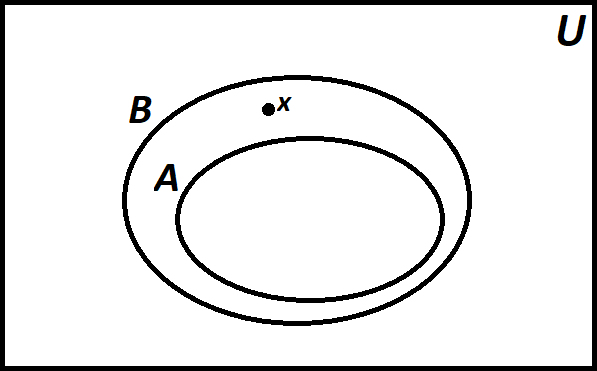
\includegraphics[width = 7 cm]{figures/sets/fig-sets-02-00.png}
      \caption{O conjunto $A$ está contido no conjunto $B$, equivalentemente, $B$ contém $A$.}
      \label{fig:sets-02-00}
  \end{figure}

  \textbf{Interseção:} Se estamos interessados em conjuntos/elementos que pertencem simultaneamente a dois conjuntos $A$ e $B$, dizemos que estamos interessados na interseção de $A$ e $B$ (denotada como $A \cap B$)$^{\ref{fig:sets-02-01}}$.
  
  \begin{figure}[hbt!]
      \centering      
      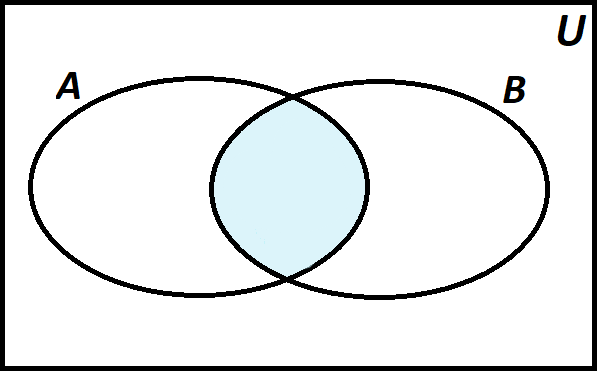
\includegraphics[width = 7 cm]{figures/sets/fig-sets-02-01.png}
      \caption{A região azul representa a visualização da interseção dos conjuntos $A$ e $B$.}
      \label{fig:sets-02-01}
  \end{figure}
  
  \textbf{União:} Já se estamos interessados nos conjuntos/elementos que fazem parte de $A$ ou de $B$ dizemos que, nosso objetivo é a união de $A$ e $B$ ($A \cup B$)$^{\ref{fig:sets-02-02}}$.
  
  \begin{figure}[hbt!]
      \centering      
      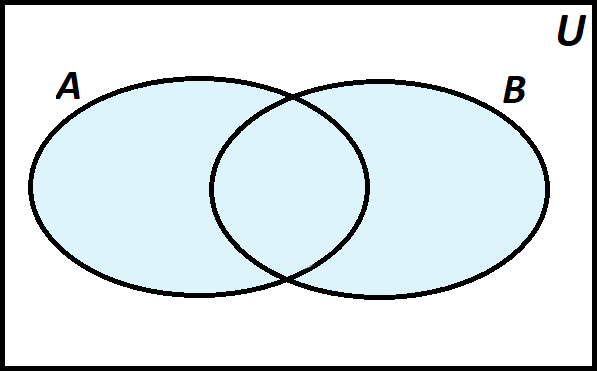
\includegraphics[width = 7 cm]{figures/sets/fig-sets-02-02.png}
      \caption{A região azul representa a visualização da união dos conjuntos $A$ e $B$.}
      \label{fig:sets-02-02}
  \end{figure}
  
  \textbf{Universo:} Quando estamos trabalhando com conjuntos é comum definirmos quem é nosso universo ($ \mathcal U $), isto é, o conjunto que conterá todos os conjuntos/elementos que estaremos trabalhando em um contexto$^{\ref{fig:sets-02-03}}$. Por exemplo, na reta real nosso universo é $\mathcal U = \mathbb{R}$.
  
  \begin{figure}[hbt!]
      \centering      
      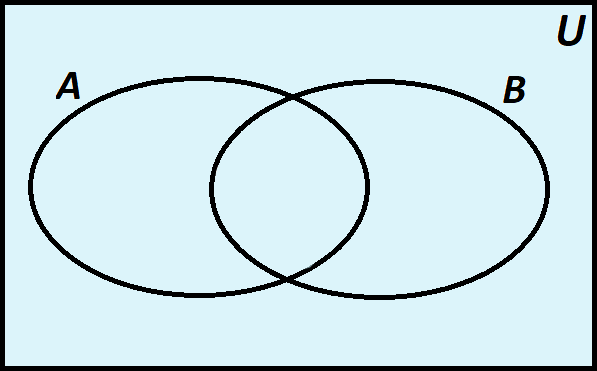
\includegraphics[width = 7 cm]{figures/sets/fig-sets-02-03.png}
      \caption{A região azul representa a visualização do nosso Universo.}
      \label{fig:sets-02-03}
  \end{figure}
  
  \textbf{Conjunto Complementar:} Sendo $A$ um conjunto, dizemos que o conjunto $A$ complementar ou complemento de $A$ (denotado como $\overline A$ ou $A^C$)contém todos os conjuntos/elementos que não estão contidos/pertencem a $A$, mas fazem parte de nosso universo ($\mathcal U$)$^{\ref{fig:sets-02-04}}$.
  
  \begin{figure}[hbt!]
      \centering      
      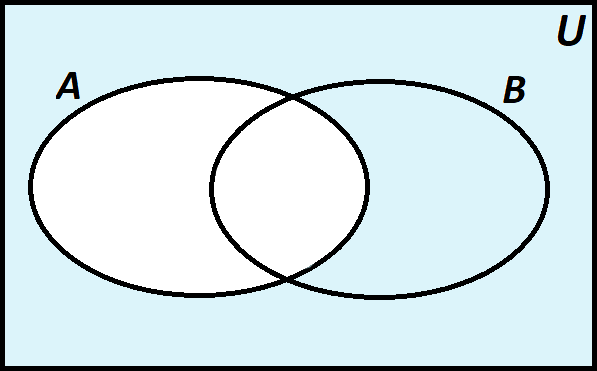
\includegraphics[width = 7 cm]{figures/sets/fig-sets-02-04.png}
      \caption{A região azul representa a visualização do complemento de $A$.}
      \label{fig:sets-02-04}
  \end{figure}
  
  \textbf{Diferença de Conjuntos :} Quando temos dois conjuntos e nosso objetivo são os conjuntos/elementos que pertencem a um destes conjuntos, mas não do outro dizemos que estamos interessados na diferença destes conjuntos. No caso, se quero os conjuntos/elementos de $B$, mas não queremos pegar os que também pertencem a $A$, queremos os elementos/conjuntos que pertencem a diferença de $B$ com $A$ (denotamos como $B-A$ ou $B \backslash A$)$^{\ref{fig:sets-02-05}}$.
  
  \begin{figure}[hbt!]
      \centering      
      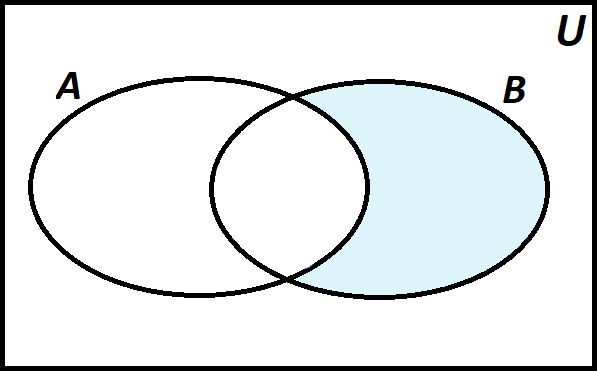
\includegraphics[width = 7 cm]{figures/sets/fig-sets-02-05.png}
      \caption{A região azul representa a visualização da diferença entre os conjuntos $B$ e $A$, isto é, a área onde estão os elementos que pertencem a $B$, mas não pertencem a $A$.}
      \label{fig:sets-02-05}
  \end{figure}
  
  Lembre-se: os diagramas apresentados servem como ferramenta auxiliar para ajudar a entender os conceitos, mas não devem ser vistos como a única ferramenta para compreender as definições e  a teoria exposta.
    
  \subsection{Definições}
  Seja $A$ e $B$ conjuntos ($\mathcal{U}$ nosso universo e $\emptyset$ o conjunto vazio, como definidos anteriormente). Assim temos, formalmente:

  \begin{itemize}
    \item \textbf{Diferença}: $A \backslash B = \{x | x \in A \land x \notin B\}$
  
    \item \textbf{Complementar}: $\overline A = \mathcal{U} \backslash A = \{x | x \in \mathcal{U} \land x \notin A\}$
  \end{itemize} 

  \subsection{Axiomas}
  Agora iremos apresentar alguns axiomas que servirão como base para todo o desenvolvimento dos conteúdos aqui propostos. Quando utilizarmos a palavra elemento, estaremos utilizando-a com a ideia de que um conjunto que pertença a outro é um elemento do segundo, para evitar repetir o uso excessivo da palavra conjunto.
  
  \textbf{Axioma da Extensionalidade:} Dois conjuntos são iguais, se e somente se, todo elemento que pertence ao primeiro conjunto pertence ao segundo e todo elemento que pertence ao segundo também pertence ao primeiro, ou seja:
  
  \[\forall A \hspace{1.5mm} \forall B \hspace{1.5mm} (A = B) \iff (\forall x \hspace{1.5mm} (x \in A \iff x \in B))\] 
  
  Através desse axioma fica mais claro de entender duas propriedades dos conjuntos. 
  
  Deste axioma, vem a explicação do motivo de que a ordem dos elementos de um conjunto não importa. Pois dado dois conjuntos com os mesmos elementos, mas em ordem diferente (por exemplo, $X=\{a,b,c,d,e,f\}$ e o conjunto $Y=\{e,c,f,b,a,d\}$) eles ainda satisfazem a propriedade de que se $t$ pertence a um deles implica $t$ pertencer ao outro. Outro ponto interessante é que não importa se um conjunto possui elementos repetidos ele continuará igual ao que possui apenas um elemento, isto é, $X=\{a,b,d,e\}$ é igual ao $Y=\{b,a,d,a,e,b,b\}$. Ou seja, em um conjunto não importa a ordem e nem as repetições de elementos.
  
  \textbf{Axioma da Existencia do Conjunto Vazio: } Diremos que no nosso universo ($\mathbb{U}$), existe um conjunto tal que ele não contém ninguém, ou seja, ele é vazio, daí seu nome, Conjunto Vazio (denotado por $\emptyset$). O axioma é:
      
    \[\exists A \hspace{1.5mm} \forall x \hspace{1.5mm} \neg\hspace{0.5mm} (x \in A)\]
  
  \textbf{Unicidade do Conjunto Vazio}
  
  Podemos provar a unicidade do conjunto vazio a partir dos dois axiomas acimas, suponhamos que existam dois conjuntos ($A$ e $B$) com a propriedade do conjunto vazio, assim utilizando o axioma da Extensão concluíremos que eles são iguais, suponhamos $t$ arbitrário:
  
  \begin{center}
      \begin{landscape}
      \AxiomC{$\forall a  \forall b  (a = b) \iff (\forall x  (x \in a \iff x \in b))$}
      \UnaryInfC{$(A = B) \iff (\forall x  (x \in A \iff x \in B))$}
      \AxiomC{$t \in A $}
      \AxiomC{}
      \RightLabel{\scriptsize $1$}
      \UnaryInfC{$\forall x \neg (x \in A)$}
      \UnaryInfC{$\neg (t \in A)$}
      \BinaryInfC{$\perp$}
      \UnaryInfC{$t \in B$}
      \AxiomC{$t \in B$}
      \AxiomC{}
      \RightLabel{\scriptsize $1$}
      \UnaryInfC{$\forall x \neg (x \in B)$}
      \UnaryInfC{$\neg (t \in B)$}
      \BinaryInfC{$\perp$}
      \UnaryInfC{$t \in A$}
      \RightLabel{\scriptsize $\iff I_1$}
      \BinaryInfC{$t \in A \iff t \in B$}
      \UnaryInfC{$\forall x  (x \in A \iff x \in B)$}
      %\RightLabel{\scriptsize $\to E_4$}
      \BinaryInfC{A=B}
      \DisplayProof
      \end{landscape}
  \end{center}

  \textbf{Axioma do Par: } Este axioma nos diz que para todos os conjuntos $A$ e $B$, existe um conjunto conjunto que é $\{A,B\}$. Ou seja,
  
    \[\forall A \hspace{1.5mm} \forall B \hspace{1.5mm} \exists C \hspace{1.5mm} \forall x \hspace{1.5mm} (x \in C \leftrightarrow x = A \vee x = B)\]
      
  Vale ressaltar que se $A=B$, teremos $\{A,B\}=\{A,A\}=\{A\}$. A aplicação sucessiva deste axioma nos permite criar uma infinidade de conjuntos finitos. Por exemplo, $A=\emptyset$ e seja $B=\emptyset$, assim teremos $\{\emptyset\}$, sendo $B=\{\emptyset\}$, teremos agora $\{\emptyset,\{\emptyset\}\}$, agora fazendo $A=\{\emptyset\}$, teremos $\{\{\emptyset\}\}$.
  
  Não pretendemos nos aprofundar mais nos axiomas de conjuntos, dado que eles utilizarão conceitos abordados futuramente, nos capítulos de Relações, Funções e Axiomas.
  
  Mas como se pode ver em ..., podemos reduzir uma grande gama de coisas a conjuntas, assim podemos tratá-las na Teoria dos Conjuntos. Para saber mais sobre Teoria dos Conjuntos dê uma olhada em ... .

\section{Diagrama de Venn}
A maneira mais simples de entender a Teoria de Conjuntos, talvez seja o Diagrama de Venn. Criado por John Venn em 1880, esse sistema de representar graficamente conjuntos auxilia imensamente quem está começando a aprender esse assunto, principalmente para entender sobre a parte inicial de notações. Basicamente, consiste em representar num plano, o universo $\mathcal U$ como sendo um retângulo e cada conjunto $A,B,...$ como uma curva fechada simples (geralmente, círculo).
    
  \subsection{Para 1 ou 2 conjuntos}
  Começando com a ideia mais simples, a imagem abaixo representa em vermelho o conjunto $A$ dentro do universo $\mathcal U$:
  
  %\begin{figure}[h!]
  %    \centering
  %    \includegraphics{fig_set_01_01.png}
  %    \caption{Conjunto $A$ dentro de $\mathcal U$}
  %    \label{fig:fig_set_01_01}
  %\end{figure}
  
  Já sobre o conjunto complementar $A^c$, ele simplesmente é a parte que está no retângulo, mas não está no círculo, justamente o que não estava de vermelho na figura anterior.
  
  %\begin{figure}[h!]
  %    \centering
  %    \includegraphics{fig_set_01_02.png}
  %    \caption{Conjunto complementar $A^c$}
  %    \label{fig:fig_set_01_02}
  %\end{figure}
  
  Para representar que um elemento pertence ao conjunto $A$, simplesmente colocamos ele dentro do espaço delimitado pelo círculo que representa o conjunto, e para representar que um elemento nāo pertence ao conjunto $A$, fazemos o inverso.
  
  
  %\begin{figure}[h!]
  %    \centering
  %    \includegraphics{figure_set_01_03.png}
  %    \caption{$a \in A$ e $b \notin A$}
  %    \label{fig:figure_set_01_03}
  %\end{figure}
  
  Quando vamos representar mais de um conjunto em um diagrama de Venn, devemos necessariamente ter todas as possíveis relações, mas o que isso significa? Por exemplo, quando temos $2$ conjuntos $A$ e $B$, significa que devemos ter $4$ regiões representando respectivamente: elementos que pertencem somente à $A$, elementos que pertencem somente à $B$, elementos que pertencem à $A$ e à $B$ simultaneamente e elementos que não pertencem a nenhum dos conjuntos. Precisamos disso, para que tudo que provarmos para dois conjuntos $A$ e $B$, possa ser generalizado para dois conjuntos quaisquer, independente do problema e da situação que estamos estudando.
  
  Utilizando esse artífiico, podemos representar todas as definições de intersecçāo, uniāo e diferença de $2$ conjuntos, introduzidas na seçāo anterior. Veja nas figuras abaixo:
  
  %\begin{figure}[h!]
  %    \centering
  %    \includegraphics{figure_set_01_04.png}
  %    \caption{Intersecção $A \cap B$}
  %    \label{fig:figure_set_01_04}
  %\end{figure}
  
  %\begin{figure}[h!]
  %    \centering
  %    \includegraphics{figure_set_01_05.png}
  %    \caption{União $A \cup B$}
  %    \label{fig:figure_set_01_05}
  %\end{figure}
  
  %\begin{figure}[h!]
  %    \centering
  %    \includegraphics{figure_set_01_06.png}
  %    \caption{Diferença $A \setminus B$}
  %    \label{fig:figure_set_01_06}
  %\end{figure}
  
  Todavia, isso ainda não permite fazer tudo que desejamos. Se quisermos representar que $A \subseteq B$, a ideia inicial seria colocar o círculo $A$ dentro do círculo $B$, quebrando o rigor de manter todas as possíveis relações, pois não teremos uma região para representar os elementos que pertecem somente a $A$. Então, como resolver esse problema? Representamos os conjuntos $A$ e $B$ da mesma forma que anteriormente e também escrevemos o símbolo do conjunto vazio $\emptyset$ na região dos elementos que pertencem somente a $A$. Assim, só existem elementos no conjunto $A$ que estão na região $A\cap B$, ou seja, se um elemento está em $A$, como consequência ele está em $B$, exatamente a definição de $A \subseteq B$.
  
  %\begin{figure}[h!]
  %    \centering
  %    \includegraphics{figure_set_01_07.png}
  %    \caption{Subconjunto $A \subseteq B$}
  %    \label{fig:figure_set_01_07}
  %\end{figure}
  
  É inegável que para muitos exemplos isso se torna inviável, principalmente quando o único objetivo é fazer uma ilustração matemática do problema, como por exemplo: tomamos o universo $\mathcal U$ como a fauna do nosso planeta, nele temos dois conjuntos $A$ de humanos e $B$ de mamíferos. É previamente conhecido que todos os humanos são mamíferos, falando de outra forma, que $A \subseteq B$. Logo, pra representar um problema que envolva esses elementos, podemos utilizar o \textbf{Diagrama de Euler}, similar ao Diagrama de Venn, com a diferença de que não é necessário mostrar todas as possíveis relações, mas apenas as relações específicas do problema retratado. E assim, fazemos exatamente o que tinha sido proposto no parágrafo anterior e, colocar o círculo $A$ dentro do círculo $B$.

  %\begin{figure}[h!]
  %    \centering
  %    \includegraphics{figure_set_01_08.png}
  %    \caption{Diagrama de Euler $A \subseteq B$}
  %    \label{fig:figure_set_01_08}
  %\end{figure}

  \subsection{Para 3 conjuntos ou mais}    
  Já foi bastante falado sobre Diagrama de Venn, mas nem chegamos a trabalhar com mais de $2$ conjuntos, o que é importante, dado que a Teoria de Conjuntos não se resume a $A$ e $B$. Mas antes de partirmos para mais conjuntos, vamos pensar numa generalização de quantas regiões diferentes devemos ter para que o diagrama seja um Diagrama de Venn. Dado $n$ conjuntos diferentes, tomamos um elemento qualquer $x$, e para cada um dos $n$ conjuntos existem duas possibilidades: $x \in $ conjunto e $x \notin $ conjunto. Logo, concluímos que existem $\underbrace{\begin{matrix} 2\cdot2\cdots2\cdot2\end{matrix}}_{n} = 2^n$ possibilidades de pertencimento de $x$ nos conjuntos, equivalente à dizer que existem $2^n$ regiões diferentes. Isso bate perfeitamente com o caso anterior pra $2$ conjuntos, pois vimos que era necessário ter $4=2^2$ regiões diferentes.

  Agora, com $3$ conjuntos $A$, $B$ e $C$, o número de regiões diferentes é $2^3=8$, mas como iremos representá-las? A primeira ideia que vem a cabeça é adicionar um círculo representando o conjunto $C$ no diagrama da figura $\ref{fig:sets-02-00}$, intersectando as regiões já existentes, resultando na figura abaixo:

  Fazendo uma rápida contagem, obtemos $8$ regiões diferentes, exatamente como deve ser (lembrete: A região fora dos conjuntos mas dentro do universo $\mathcal U$, também é considerada na contagem). E da mesma forma que representamos intersecção, união e diferença de conjuntos anteriormente, também podemos representar com $3$ conjuntos, veja abaixo:

  %\begin{figure}[h!]
  %    \centering
  %    \includegraphics{figure_set_01_09.png}
  %    \caption{Intersecção $A \cap B \cap C$}
  %    \label{fig:figure_set_01_09}
  %\end{figure}

  %\begin{figure}[h!]
  %    \centering
  %    \includegraphics{figure_set_01_10.png}
  %    \caption{União $A \cup B \cup C$}
  %    \label{fig:figure_set_01_10}
  %\end{figure}

  %\begin{figure}[h!]
  %    \centering
  %    \includegraphics{figure_set_01_11.png}
  %    \caption{Diferença $A \setminus (B \cup C)$}
  %    \label{fig:figure_set_01_11}
  %\end{figure}

  Sendo ganancioso e indo além, podemos querer representar $4$ conjuntos, adicionando o conjunto $D$. E igual o caso anterior, só temos que adicionar mais um círculo representando o conjunto $D$ e, dado que antes obtemos um triângulo de círculos, dessa vez iremos ter uma quadrado de cícurlos, correto?

  \textbf{ERRADO!} Se você é um leitor observador, já deve ter notado que esse diagrama não possui as $2^4=16$ regiões diferentes necessárias, mas somente $14$. Não existem regiões que representam os elementos que pertencem ao mesmo tempo aos conjuntos $A$ e $D$, mas não pertencem ao conjunto $B$ e nem ao $C$, e o inverso disso, ou seja, os elementos que pertencem ao mesmo tempo aos conjuntos $B$ e $C$, mas não pertencem ao conjunto $A$ e nem ao $D$.

  É válido ressaltar que é impóssível utilizar $4$ círculos pra representar $4$ conjuntos em um diagrama de Venn. Contudo, existem diagramas de Venn pra $4$ conjuntos, e antes de ler o próximo parágrafo, pegue uma folha e tente encontrar possíveis maneiras dessa representação. Dica: Não se abstenha de utilizar formas bem diferenciadas. 
  
  Se você conseguiu, parabéns. Saiba que existem diversas maneiras, como por exemplo: $4$ elipses ou $3$ círculos e uma forma semelhante à metade de uma rosquinha. Fique a vontade para pesquisar na internet essas e outras maneiras de representação. Ainda assim, é relevante mostrar pelo menos uma delas, e escolhemos a da figura abaixo, muito semelhante a dois corações.

  %\begin{figure}[h!]
  %    \centering
  %    \includegraphics{figure_set_01_11.png}
  %    \caption{Diagrama de Venn para 4 conjuntos}
  %    \label{fig:figure_set_01_11}
  %\end{figure}

  Podemos continuar e encontrar representações para $5$ ou mais conjuntos, as quais vão ficando cada vez mais complicadas. Porém, como nosso principal objetivo é utilizar visualizações gráficas para facilitar o aprendizado em Teoria de Conjuntos, a partir do momento que isso vem a se tornar complicado, perde totalmente a utilidade. Por esse motivo, vamos parar em $4$ conjuntos, mas se a curiosidade for grande, procure aprender mais sobre esse assunto.

  \subsection{Aplicações}
  A mais importante e útil das aplicações é justamente demonstrar propriedades da Teoria de Conjuntos. Se fosse solicitado para você leitor demonstrar as propriedades a seguir, somente com o que aprendeu até agora, já conseguiria utilizar o Diagrama de Venn para demonstrá-las. Apesar de parecer complicado, é incrivelmente simples, veja:
  
  \textbf{Exemplo 1:} Demonstre que $A \setminus B = A \cap B^c$.

  \textbf{Resposta:} Primeiramente, vamos fazer o Diagrama de Venn desses dois conjuntos e enumerar as $4$ regiões:

  %\begin{figure}[h!]
  %    \centering
  %    \includegraphics{figure_set_01_12.png}
  %    \caption{Regiões 1, 2, 3 e 4}
  %    \label{fig:figure_set_01_12}
  %\end{figure}

  Assim, temos que $A=\{1,2\}$, $B=\{2,3\}$, $A^c=\{3,4\}$ e $B^c=\{1,4\}$. Utilizando esse valores, podemos calcular $A \setminus B$ e $A \cap B^c$, conforme abaixo:

  \begin{equation*}
    \begin{aligned}
      A \setminus B &= \{1,2\} \setminus \{2,3\} = \{1\}\\
      A \cap B^c &= \{1,2\} \cap \{1,4\} = \{1\}
    \end{aligned}
  \end{equation*}

  Portanto, concluímos que $A \setminus B = A \cap B^c$.
  
  \textbf{Exemplo 2:} Demonstre que $(A \setminus B) \cup (B \setminus A) = (A \cup B) \setminus (A \cap B)$.

  \textbf{Resposta:} Utilizando o mesmo Diagrama de Venn e a mesma numeração de regiões do exemplo anterior, temos:

  \begin{equation*}
    \begin{aligned}
      A \setminus B &= \{1,2\} \setminus \{2,3\} = \{1\}\\
      B \setminus A &= \{2,3\} \setminus \{1,2\} = \{3\}\\
      A \cup B &= \{1,2\} \cup \{2,3\} = \{1,2,3\}\\
      A \cap B &= \{1,2\} \cap \{2,3\} = \{2\}\\
      (A \setminus B) \cup (B \setminus A) &= \{1\} \cup \{3\} = \{1,3\}\\
      (A \cup B) \setminus (A \cap B) &= \{1,2,3\} \setminus \{2\} = \{1,3\}
    \end{aligned}
  \end{equation*}
  
  Portanto, concluímos que $(A \setminus B) \cup (B \setminus A) = (A \cup B) \setminus (A \cap B)$.
  \newline
  É possível responder essas questões somente utilizando o diagrama e pintando as regiões, mas a enumeração torna o processo mais fácil.
  
  $\qquad$

  Outra aplicação interessante, muito recorrente em testes de lógica e vestibulares, é tentar interpretar problemas da vida real com conjuntos, conforme no exemplo a seguir.

  \textbf{Exemplo 3:} Em uma sala de aula do Ensino Fundamental com $40$ alunos, a professora Ana perguntou quem gostava de matemática e quem gostava de português. Ela obteve os seguintes dados:

  \begin{itemize}
    \item $21$ alunos gostam de matemática
    \item $17$ alunos gostam de português
    \item $9$ alunos não gostam de nenhuma das matérias
  \end{itemize}

  Quantos alunos gostam de ambas as matérias?

  \textbf{Resposta:} Vamos utilizar um Diagrama de Venn para dois conjuntos, onde um conjunto representa os alunos que gostam de matemática e o outro representa os que gostam de português.
  Dado que $9$ alunos não gostam de nenhuma das matérias e temos $40$ alunos na sala, então $40-9=31$ alunos pertencem a pelo menos um dos conjuntos, ou seja, gostam de matemática ou português.

  Como $21$ gostam de matemática, logo $31-21=10$ gostam somente de português (região da esquerda) e, analogamente, como $17$ gostam de português, logo $31-17=14$ gostam somente de matemática (região da direita). Utilizando esses dados, vemos que ainda faltam $31-10-14=7$ alunos, justamente os que gostam de ambas as matérias (região do meio). Veja abaixo o diagrama final:

  %\begin{figure}[h!]
  %    \centering
  %    \includegraphics{figure_set_01_13.png}
  %    \caption{Diagrama de Venn para Matemática e Português}
  %    \label{fig:figure_set_01_13}
  %\end{figure}

  $\qquad$

  Apesar do estudo de conjuntos com Diagrama de Venn ser fácil, simples e útil, como já comentado anteriormente, é difícil para trabalhar com muitos conjuntos, além das provas utilizando esse recurso não terem um grau de formalidade muitas vezes requerido pelos matemáticos. Devido a esse fato, iremos estudar nas próximas seções outras maneiras de lidar com Teoria dos Conjuntos, como provas matemáticas formais, dedução natural, cálculo em conjuntos e é claro, utilizando o Lean.

\section{Prova de Teoremas}
Nesta seção iremos tratar de formalizar definições e Teoremas. Ao contrário da seção $5.2$, onde o foco era transmitir a notação e uma ideia geral dos conceitos.

Aqui serão apresentadas algumas provas em Lean para o conteúdo apresentado. Não se preocupe, caso não entenda sobre o que o código quer dizer ignore ele por enquanto e após ler as próximas duas seções (que falam de conjuntos em Lean), volte e tente compreender o que foi feito. Já que o foco principal nesta parte são as provas matemáticas tradicionais e as definições mais precisas.

  \subsection{Prova Matemática Formal}
  Ainda vai ter algo escrito aqui

  \subsection{Dedução Natural}
  Ainda vai ter algo escrito aqui

\section{Conjuntos em Lean}
Embora na teoria axiomática dos conjuntos se considere conjuntos de objetos distintos, em matemática é mais comum considerar subconjuntos de algum dominio fixo ($\mathcal U $). É assim que os conjuntos são tratados em Lean. Para qualquer dado do tipo $U$, Lean nos retorna um novo dado tipo $conjunto$ $U$, que consiste no conjunto dos elementos de $U$. Assim, por exemplo, podemos raciocinar sobre conjuntos de números naturais, conjuntos de números inteiro ou conjuntos de pares de números naturais.

  \subsection{Notações}
  O lean possui uma biblioteca padrão para lidar com conjuntos chamada set e, sempre que formos utilizar um comando que pertence à ela, é necessário escrever {\fontencoding{U}\fontfamily{cmtt}\selectfont set.comando}. Entretanto, pra facilitar nossa vida, podemos escrever {\fontencoding{U}\fontfamily{cmtt}\selectfont open set} no início do código, o que permite escrevermos somente {\fontencoding{U}\fontfamily{cmtt}\selectfont comando}, e o lean já entende que ele pertence a biblioteca set.
  
  Além disso, para trabalharmos com conjuntos, também é essencial definirmos um tipo {\fontencoding{U}\fontfamily{cmtt}\selectfont U} e sabermos utilizar conjuntos e elementos desse tipo. Para isso, utilizamos o código abaixo:

  \begin{lstlisting}
  open set

  variable {U : Type}
  variables A B C : set U
  variable x : U \end{lstlisting}

  Temos aqui uma pequena lista de como se representa os principais caractéres da parte de conjuntos em Lean: 

  \begin{itemize}
      \item $\in$ $\rightarrow$ $\backslash$in
    
      \item $\notin$ $\rightarrow$ $\backslash$notin
    
      \item $\subset$ $\rightarrow$ $\backslash$subset
    
      \item $\subseteq$ $\rightarrow$ $\backslash$sub
    
      \item $\emptyset$ $\rightarrow$ $\backslash$empty
    
      \item $\cup$ $\rightarrow$ $\backslash$un \ ou \ $\backslash$cup \ ou \ $\backslash$union
    
      \item $\cap$ $\rightarrow$ $\backslash$i \ ou \ $\backslash$cap \ ou \ $\backslash$intersection
  \end{itemize}

  Obs$^{1}$.: O conjunto universal é denotado {\fontencoding{U}\fontfamily{cmtt} \selectfont univ}.

  Obs$^{2}$.: O complementar de um conjunto é denotado com um símbolo de negação antes de seu símbolo, assim: $-A$

  Podemos ver alguns exemplos abaixo:
  \begin{lstlisting}
    open set
    variable {U : Type}
    variables A B C : set U
    variable x : U

    #check x ∈ A
    #check A ∪ B
    #check B \ C
    #check C ∩ A
    #check -C
    #check ∅ ⊆ A
    #check B ⊆ univ \end{lstlisting}

  Noções básicas da teoria dos conjuntos são definidas na biblioteca principal do Lean, mas teoremas e notações adicionais que iremos utilizar nesse capítulo, estão disponíveis em uma biblioteca auxiliar que é carregada com o comando 
  {\fontencoding{U}\fontfamily{cmtt} \selectfont import data.set}, o qual deve aparecer no início do arquivo.

  \begin{lstlisting}
    import data.set
    open set
    variable {U : Type}
    variables A B C : set U
    variable x : U \end{lstlisting}

  A partir desse momento, para evitar repetição, iremos omitir as $4$ primeiras linhas do código, no entanto \textbf{você deve lembrar que elas existem para seu código funcionar.} Já sobre a linha $5$, não é necessário escrever nos próximos exemplos, pois sempre iremos se referenciar a um elemento do tipo{\fontencoding{U}\fontfamily{cmtt} \selectfont U}, dentro de {\fontencoding{U}\fontfamily{cmtt}\selectfont example, lemma} ou {\fontencoding{U}\fontfamily{cmtt}\selectfont theorem}.

  \subsection{Primeiros Passos}

  Relembrando a definição de subconjunto, podemos utilizar o template abaixo para mostrar que o conjunto $A$ é um subconjunto de $B$:

  \begin{lstlisting}
  example : A ⊆ B :=
  assume x : U,
  assume h : x ∈ A,
  show x ∈ B, from sorry \end{lstlisting}

  Obs: Na linha $2$ poderíamos ter escrito somente {\fontencoding{U}\fontfamily{cmtt}\selectfont assume x}, pois já inferiria que {\fontencoding{U}\fontfamily{cmtt}\selectfont x} é do tipo {\fontencoding{U}\fontfamily{cmtt}\selectfont U}.

  Já para mostrar que $A$ e $B$ são iguais, temos dois comandos diferentes: {\fontencoding{U}\fontfamily{cmtt}\selectfont eq\_of\_subset\_of\_subset} e {\fontencoding{U}\fontfamily{cmtt}\selectfont ext}.

  \textbf{eq\_of\_subset\_of\_subset:} Ele funciona interpretando a seguinte expressão $(A \subseteq B \wedge B \subseteq A) \Rightarrow A=B$, ou seja, obtém a equivalência dos conjuntos a partir do fato de que o primeiro é subconjunto do segundo, e vice-vera. Veja o código:

  \begin{lstlisting}
  example : A = B :=
  eq_of_subset_of_subset
    (assume x,
      assume h : x ∈ A,
      show x ∈ B, from sorry)
    (assume x,
      assume h : x ∈ B,
      show x ∈ A, from sorry) \end{lstlisting}

  \textbf{ext:} É uma sigla para ``extensionality", ou seja, extensionalidade. Matemáticamente, isso representa a expressão $\forall x \ (x \in A \leftrightarrow x \in B) \Rightarrow A=B$. Veja o código:

  \begin{lstlisting}
  example : A = B :=
  ext (assume x, iff.intro
    (assume h : x ∈ A,
      show x ∈ B, from sorry)
    (assume h : x ∈ B,
      show x ∈ A, from sorry)) \end{lstlisting}

  Além disso, o Lean possui interpretação ambígua para regras de união, interseção e outras operações em conjuntos que são consideradas “definições”. Isso significa que as expressões $x$ $\in$ $A$ $\cap$ $B$ e $x$ $\in$ $A$ $\wedge$ $x$ $\in$ $B$ possuem a mesma interpretação no Lean. Isso também é válido para outras construções em conjuntos, como: $x$ $\in$ $A$ $\backslash $ $B$ e $x$ $\in$ $A$ $\wedge$ $\neg$ $(x$ $\in$ $B)$. O termo $\neg$ $(x$ $\in$ $B)$ é somente outra forma de escrever $x$ $\notin$ $B$. Abaixo são apresentadas algumas aplicações dessa interpretação:

  \begin{lstlisting}
  example : ∀ x, x ∈ A → x ∈ B → x ∈ A ∩ B :=
  assume x,
  assume h₁ : x ∈ A,
  assume h₂ : x ∈ B,
  show x ∈ A ∩ B, from and.intro h₁ h₂

  example : A ⊆ A ∪ B :=
  assume x,
  assume h : x ∈ A,
  show x ∈ A ∪ B, from or.inl h

  example : ∅ ⊆ A  :=
  assume x,
  assume h : x ∈ (∅ : set U),
  show x ∈ A, from false.elim h \end{lstlisting}

  Observe no último exemplo a necessidade de usar a notação {\fontencoding{U}\fontfamily{cmtt} \selectfont ($\emptyset$ : set U)}, dizendo ao nosso provador que o $\emptyset$ é um conjunto de {\fontencoding{U}\fontfamily{cmtt}
  \selectfont U}. Isso acontece pois ele não consegue inferir que tipo é o conjunto vazio, dado que por definição, esse conjunto existe em qualquer universo, ou seja, pode ser de qualquer tipo.

  Opcionalmente, podemos usar alguns teoremas da biblioteca {\fontencoding{U}\fontfamily{cmtt}
  \selectfont data.set}, projetados especificamente para uso em conjuntos:

  \begin{lstlisting}
  example : ∀ x, x ∈ A → x ∈ B → x ∈ A ∩ B :=
  assume x,
  assume : x ∈ A,
  assume : x ∈ B,
  show x ∈ A ∩ B, from mem_inter ‹x ∈ A› ‹x ∈ B›

  example : A ⊆ A ∪ B :=
  assume x,
  assume h : x ∈ A,
  show x ∈ A ∪ B, from mem_union_left B h

  example : ∅ ⊆ A  :=
  assume x,
  assume : x ∈ ∅,
  show x ∈ A, from absurd this (not_mem_empty x) \end{lstlisting}

  Lembre-se que o comando{\fontencoding{U}\fontfamily{cmtt}
  \selectfont absurd} pode ser usado para provar qualquer fato a partir de duas hipóteses contrárias: $h_1$ : $P$ e $h_2$ : $\neg$ $P$. 

  Aqui, o teorema {\fontencoding{U}\fontfamily{cmtt}
  \selectfont not\_mem\_empty x} significa $x$ $\notin$ $\emptyset$. Para ver a declaração de teoremas disponíveis, utilize o comando{\fontencoding{U}\fontfamily{cmtt}
  \selectfont \#check}:

  \begin{lstlisting}
  #check @mem_inter
  #check @mem_of_mem_inter_left
  #check @mem_of_mem_inter_right
  #check @mem_union_left
  #check @mem_union_right
  #check @mem_or_mem_of_mem_union
  #check @not_mem_empty \end{lstlisting}

  Neste caso, o símbolo{\fontencoding{U}\fontfamily{cmtt}
  \selectfont @} impede que ele tente preencher argumentos implícitos automaticamente, forçando-o a exibir a declaração completa do teorema.

  Já que podemos relacionar conjuntos com suas definições lógica, isso auxilia a comprovação de inclusões entre conjuntos:

  \begin{lstlisting}
  example : A \ B ⊆ A :=
  assume x,
  assume : x ∈ A \ B,
  show x ∈ A, from and.left this

  example : A \ B ⊆ -B :=
  assume x,
  assume : x ∈ A \ B,
  have x ∉ B, from and.right this,
  show x ∈ -B, from this \end{lstlisting}

  Novamente, é possível usar versões dos teoremas projetados especificamente para conjuntos:

  \begin{lstlisting}
  example : A \ B ⊆ A :=
  assume x,
  assume : x ∈ A \ B,
  show x ∈ A, from mem_of_mem_diff this

  example : A \ B ⊆ -B :=
  assume x,
  assume : x ∈ A \ B,
  have x ∉ B, from not_mem_of_mem_diff this,
  show x ∈ -B, from this \end{lstlisting}

  %Acho que a partir desse ponto, não é necessário ter nesse capítulo. Talvez seja melhor deixar só pro capítulo de propriedades. Por isso, já copiei e colei no outro capítulo. Se ainda sim quiser falar sobre como lidar com sorry, pegue algum dos exemplos já citados acima. E se quiser colocar mais coisas teóricas ou explicativas, está totalmente livre. Mas deixe as propriedades/identidades pro capítulo delas.

\section{Propriedades}
A seguir teremos algumas propriedades e a prova do porque estão corretas.
    
\begin{itemize}  
    \item $A \cup \overline A = \mathbb{U}$
\end{itemize} 

\textbf{Prova:} Seja $x$ um elemento de $A \cup \overline A$, assim temos que 
\[x \in (A \cup \overline A)\]
\[ \iff x \in A \vee x \in \overline A\]
    
\begin{itemize}
    \item $A \cap \overline A = \empty{U}$
\end{itemize} 

\textbf{Prova:} Seja $x$ um elemento de $A \cap \overline A$, assim:

$(i)$ Provaremos que $ \forall x (x \in A \cap \overline A) \rightarrow \forall x  (x \in \emptyset) $ :

\begin{center}
    \AxiomC{}
    \RightLabel{\scriptsize $1$}
    \UnaryInfC{$ \forall x (x \in A \cap \overline A)$}
    \UnaryInfC{$t \in A \cap \overline A$}
    \UnaryInfC{$t \in A \land t \in \overline A $}
    \UnaryInfC{$t \in A $}
    \AxiomC{}
    \RightLabel{\scriptsize $1$}
    \UnaryInfC{$ \forall x (x \in A \cap \overline A)$}
    \UnaryInfC{$t \in A \cap \overline A$}
    \UnaryInfC{$t \in A \land t \in \overline A $}
    \UnaryInfC{$t \in \overline A $}
    \UnaryInfC{$t \in \mathbb{U} \land t \notin A $}
    \UnaryInfC{$t \notin A $}
    \BinaryInfC{$\perp$}
    \UnaryInfC{$t \in \emptyset$}
    \UnaryInfC{$\forall x  (x \in \emptyset)$}
    \RightLabel{\scriptsize $1$}
    \UnaryInfC{$ \forall x (x \in A \cap \overline A) \rightarrow \forall x  (x \in \emptyset) $}
    \DisplayProof
\end{center}
    
$(ii)$ Provaremos que $ \forall x  (x \in \emptyset) \rightarrow \forall x (x \in A \cap \overline A)$ :
\begin{center}
    \AxiomC{}
    \RightLabel{\scriptsize $1$}
    \UnaryInfC{$\forall x  (x \in \emptyset)$}
    \UnaryInfC{$\perp$}
    \UnaryInfC{$t \in A \cap \overline A$}
    \UnaryInfC{$ \forall x (x \in A \cap \overline A)$}
    \RightLabel{\scriptsize $1$}
    \UnaryInfC{$\forall x  (x \in \emptyset) \rightarrow \forall x (x \in A \cap \overline A)$}
    \DisplayProof
\end{center}

Portanto, de $(i)$ e $(ii)$, concluímos que $ \forall x (x \in A \cap \overline A) \iff \forall x  (x \in \emptyset) $, ou seja, $A \cap \overline A$.

%Renan
Como o Lean tem que desenvolver definições, ele pode acabar se confundindo às vezes. Por exemplo, na prova a seguir, se você subtituir a última linha por{\fontencoding{U}\fontfamily{cmtt}
\selectfont sorry}, o Lean terá problemas tentando entender que você quer que ele desenvolva o símbolo de subconjunto:

\begin{lstlisting}
example : A ∩ B ⊆ B ∩ A :=
assume x,
assume h : x ∈ A ∩ B,
have h₁ : x ∈ A, from and.left h,
have h₂ : x ∈ B, from and.right h,
and.intro h₂ h₁ \end{lstlisting}

Uma solução alternativa é usar o comando{\fontencoding{U}\fontfamily{cmtt}
\selectfont show}. Na maioria das vezes, fornecer informações adicionais para o Lean pode ser útil. Outra solução é nomear um teorema, o que leva o Lean a usar um método um pouco diferente de processar a prova, corrigindo o problema como um efeito colateral de sorte.

\begin{lstlisting}
example : A ∩ B ⊆ B ∩ A :=
assume x,
assume h : x ∈ A ∩ B,
have h₁ : x ∈ A, from and.left h,
have h₂ : x ∈ B, from and.right h,
show x ∈ B ∩ A, from sorry

theorem my_example : A ∩ B ⊆ B ∩ A :=
assume x,
assume h : x ∈ A ∩ B,
have h₁ : x ∈ A, from and.left h,
have h₂ : x ∈ B, from and.right h,
sorry \end{lstlisting}

Parte de Identidade de Conjuntos: Nessa seção, falaremos brevemente sobre Identidades de conjuntos.

Iniciaremos com um exemplo simples: a regra da distributividade para conjuntos: $A \cup (B \cap C)$ = $(A \cup B) \cap (A \cup C)$. Uma maneira de prova-la é:


\begin{lstlisting}
import data.set
open set

variable {U : Type}
variables A B C : set U

example : A ∪ (B ∩ C) = (A ∪ B) ∩ (A ∪ C) :=
eq_of_subset_of_subset
  (assume x,
    assume h : x ∈ A ∪ (B ∩ C),
    or.elim h
      (assume h₁ : x ∈ A,
        have h₂ : x ∈ A ∪ B, from or.inl h₁,
        have h₃ : x ∈ A ∪ C, from or.inl h₁,
        show x ∈ (A ∪ B) ∩ (A ∪ C), from and.intro h₂ h₃)
      (assume h₁ : x ∈ B ∩ C,
        have h₂ : x ∈ B, from and.left h₁,
        have h₃ : x ∈ C, from and.right h₁,
        have h₄ : x ∈ A ∪ B, from or.inr h₂,
        have h₅ : x ∈ A ∪ C, from or.inr h₃,
        show x ∈ (A ∪ B) ∩ (A ∪ C), from and.intro h₄ h₅))
  (assume x,
    assume h : x ∈ (A ∪ B) ∩ (A ∪ C),
    have h₁ : x ∈ A ∪ B, from and.left h,
    have h₂ : x ∈ A ∪ C, from and.right h,
    or.elim h₁
      (assume h₃ : x ∈ A,
        show x ∈ A ∪ (B ∩ C), from or.inl h₃)
      (assume h₃ : x ∈ B,
      or.elim h₂
        (assume h₄ : x ∈ A,
        show x ∈ A ∪ (B ∩ C), from or.inl h₄)
        (assume h₄ : x ∈ C,
        have h₅ : x ∈ B ∩ C, from and.intro h₃ h₄, 
        show x ∈ A ∪ (B ∩ C), from or.inr h₅)))
\end{lstlisting}

Outra identidade que usaremos como exemplo aqui é a Lei de Absorção:  

\begin{center}
    $A \cup (A \cap B) = A$
\end{center}

Nos templates abaixo temos duas formas de escrever a prova: a que estamos utilizando ao longo deste capítulo; e em forma de lógica booleana, trocando o sinal de igual pelo de equivalência, ou ``se e somente se", ($\leftrightarrow$). (Você consegue reprentá-lo no Lean escrevendo: $\backslash$iff ou $\backslash$lr)

\begin{lstlisting}
import data.set
open set

theorem inter_subseq (H : Type)(P Q : set H) : P ∩ (P ∪ Q) = P :=
eq_of_subset_of_subset
  (assume x,
    assume h : x ∈ P ∩ (P ∪ Q),
    show x ∈ P, from h.left)
  (assume x,
    assume h : x ∈ P,
    have h₁ : x ∈ P ∪ Q, from or.inl h,
    show x ∈ P ∩ (P ∪ Q), from and.intro h h₁)

variable  U : Type
variables A B : set U

example : A ∪ (A ∩ B) = A :=
calc
  A ∪ (A ∩ B) = (A ∪ A) ∩ (A ∪ B) : by rw union_distrib_left
          ... = A ∩ (A ∪ B)       : by rw union_self
          ... = A                 : by rw inter_subseq
\end{lstlisting}

\begin{lstlisting}
import logic.basic
open classical

theorem left_of_and (P Q : Prop) : P ∧ (P ∨ Q) ↔ P :=
iff.intro
  (assume h : P ∧ (P ∨ Q),
  show P, from h.left)
  (assume h : P,
  have h₁ : P ∨ Q, from or.inl h,
  show P ∧ (P ∨ Q), from and.intro h h₁)

variables A B : Prop

example : A ∨ (A ∧ B) ↔ A :=
calc
  A ∨ (A ∧ B) ↔ (A ∨ A) ∧ (A ∨ B) : by rw or_and_distrib_left
          ... ↔ A ∧ (A ∨ B)        : by rw or_self
          ... ↔ A                  : by rw left_of_and
\end{lstlisting}

  \subsection{Básicas}
  %Pode ser separada em: Básicas, Sobre o conjunto vazio, Sobre o Universo
  Ainda vai ter algo escrito aqui

  \subsection{Comutatividade}
  Ainda vai ter algo escrito aqui

  \subsection{Associatividade}
  Ainda vai ter algo escrito aqui

  \subsection{Distributividade}
  Ainda vai ter algo escrito aqui

  \subsection{Complementar/Lei de Demorgan}
  Ainda vai ter algo escrito aqui

  \subsection{Lei da Absorção}
  Ainda vai ter algo escrito aqui

  \subsection{Extras}
  Ainda vai ter algo escrito aqui

\section{Cálculo em Conjuntos}
Primeiramente, não confunda isso com o Cálculo da matemática que envolve derivada, integral, somatório, etc. Estamos falando do cálculo essencial desde a matemática básica, geralmente usado em provas como sendo uma sequência de operações para provar que duas expressões são equivalentes.

  \subsection{Cálculo Matemático}
  Vamos utilizar o seguinte exemplo, e mesmo que não conheça-o, você já deve ter feito algo semelhante.

  \textbf{Prove que} $\dfrac{(a+b)^2+(a-b)^2}{2}-2b^2 = (a-b)(a+b)$, $\forall\ a,b$ números naturais. 

  Provavelmente a primeira ideia que uma pessoa com pouco conhecimento de álgebra tem, é desenvolver ambos os lados ao mesmo tempo, chegando em expressões iguais, como mostrado a seguir:

  \begin{equation*}
    \begin{aligned}
      \dfrac{(a+b)^2+(a-b)^2}{2}-2b^2 &=? (a-b)(a+b)\\
      \dfrac{a^2+2ab+b^2+a^2-2ab+b^2}{2}-2b^2 &=? a^2+ab-ab-b^2\\
      \dfrac{2a^2+2b^2}{2}-2b^2 &=? a^2-b^2\\
      a^2+b^2-2b^2 &=? a^2-b^2\\
      a^2-b^2 &= a^2-b^2
    \end{aligned}
  \end{equation*}

  O que fornece a impressão de que começamos com uma identidade complexa, e então, depois de muito sofrimento e muitas contas, finalmente conseguimos provar que $x=x$. Chega a ser engraçado, não é mesmo?
  Então o melhor a se fazer é justamente começar de uma igualdade do tipo $x=x$ e chegar na igualdade desejada.

  \begin{equation*}
    \begin{aligned}
      a^2-b^2 &= a^2-b^2\\
      a^2+b^2-2b^2 &= a^2-b^2\\
      \dfrac{2a^2+2b^2}{2}-2b^2 &= a^2-b^2\\
      \dfrac{a^2+2ab+b^2+a^2-2ab+b^2}{2}-2b^2 &= a^2+ab-ab-b^2\\
      \dfrac{(a+b)^2+(a-b)^2}{2}-2b^2 &= (a-b)(a+b)
    \end{aligned}
  \end{equation*}

  Se tornando mais estranho ainda! Pois agora parece que foi escolhida uma igualdade aleatória, e graças a sorte, conseguimos provar a identidade a partir dela. E não é isso que desejamos.

  Voltando a primeira prova, vemos que a ideia que tentamos transmitir é que cada equação é equivalente a seguinte, ou seja, a primeira equação é verdadeira se, e somente se, a segunda também for verdadeira. Logo, podemos utilizar o símbolo $\iff$ entre cada uma delas.

  \begin{equation*}
    \begin{aligned}
      &\dfrac{(a+b)^2+(a-b)^2}{2}-2b^2 = (a-b)(a+b)\\
      \iff &\dfrac{a^2+2ab+b^2+a^2-2ab+b^2}{2}-2b^2 = a^2+ab-ab-b^2\\
      \iff &\dfrac{2a^2+2b^2}{2}-2b^2 = a^2-b^2\\
      \iff &a^2+b^2-2b^2 = a^2-b^2\\
      \iff &a^2-b^2 = a^2-b^2
    \end{aligned}
  \end{equation*}

  Ou ainda, utilizar frases como ``basta provar'' entre uma igualdade e outra.

  Queremos provar

  \[\dfrac{(a+b)^2+(a-b)^2}{2}-2b^2 = (a-b)(a+b)\]

  Para fazer isso, basta provar

  \[\dfrac{a^2+2ab+b^2+a^2-2ab+b^2}{2}-2b^2 = a^2+ab-ab-b^2\]

  Para isso, basta provar

  \[\dfrac{2a^2+2b^2}{2}-2b^2 = a^2-b^2\]

  E para isso, basta provar

  \[a^2+b^2-2b^2 = a^2-b^2\]
  
  O que é claramente verdadeiro.
  
  $\qquad$

  Ambas as provas são mais formais, apesar da última possuir uma narrativa repetitiva que nos obriga a encontrar sinônimos para a frase ``basta provar''. Contudo, podemos ser melhores.
  
  Para facilitar, denominamos a expressão do lado esquerdo por $LE$ e a expressão do lado direito por $LD$. Assim, o que a nossa demonstração está fazendo é transformar $LE$ numa expressão $E$ e, $LD$ na mesma expressão $E$.
  Portanto, podemos reescrevê-la somente como um único cálculo direcionado para a frente, transformando $LE$ em $E$ e então, fazendo uma transformação inversa de $E$ para $LD$.

  \begin{equation*}
    \begin{aligned}
      \dfrac{(a+b)^2+(a-b)^2}{2}-2b^2 &= \dfrac{a^2+2ab+b^2+a^2-2ab+b^2}{2}-2b^2\\
      &= \dfrac{2a^2+2b^2}{2}-2b^2\\
      &= a^2+b^2-2b^2\\
      &= a^2-b^2\\
      &= a^2+ab-ab-b^2\\
      &= (a-b)(a+b)
    \end{aligned}
  \end{equation*}

  Por fim, obtemos uma prova clara, compacta e legível. Esse é o modelo mais utilizado pelos matemáticos em geral, e também é o qual utilizaremos nessa seção.

  $\qquad$

  Partindo agora para o que realmente interessa, podemos provar que dois conjuntos são iguais argumentando sobre seus elementos, conforme visto nas seções anteriores, ou podemos ser mais eficientes e utilizar o cálculo juntamente com as propriedades vistas na seção $5.6$. Veja alguns exemplos:

  \textbf{Exemplo 1:} Demonstre que $(A \setminus B)^c = A^c \cup B$

  \textbf{Prova:} Utilizando cálculo:
  \begin{equation*}
    \begin{aligned}
      (A \setminus B)^c &= (A \cap B^c)^c)\\
      &= A^c \cup (B^c)^c\\
      & = A^c \cup B
    \end{aligned}
  \end{equation*}

  $\qquad$

  Relembrando um dos exemplos da seção $5.3$:

  \textbf{Exemplo 2:} Demonstre que $(A \setminus B) \cup (B \setminus A) = (A \cup B) \setminus (A \cap B)$

  \textbf{Prova:} Utilizando cálculo:
  \begin{equation*}
    \begin{aligned}
      (A \setminus B) \cup (B \setminus A) &= (A \cap B^c) \cup (B \cap A^c)\\
      &= ((A \cap B^c) \cup B) \cap ((A \cap B^c) \cup A^c)\\
      &= ((A \cup B) \cap (B^c \cup B)) \cap ((A \cup A^c) \cap (B^c \cup A^c))\\
      &= ((A \cup B) \cap \mathcal U) \cap (\mathcal U \cap (B^c \cup A^c))\\
      &= (A \cup B) \cap (B^c \cup A^c)\\
      &= (A \cup B) \cap (A^c \cup B^c)\\
      &= (A \cup B) \cap (A \cap B)^c\\
      &= (A \cup B) \setminus (A \cap B)
    \end{aligned}
  \end{equation*}

  \subsection{Calc em Lean}
  Ainda vai ter algo escrito aqui

\section{Famílias Indexadas}

  \subsection{Definição}
  Ainda vai ter algo escrito aqui

  \subsection{Em Lean}
  Ainda vai ter algo escrito aqui

\section{Power Set}

  \subsection{Definição}
  Ainda vai ter algo escrito aqui

  \subsection{Em Lean}
  Ainda vai ter algo escrito aqui

\section{Exercícios}
\begin{enumerate}
    
\item Questões de Identidades de conjuntos
    
\begin{lstlisting}
import data.set
open set

section
  variable U : Type
  variables A B C : set U

--Comutatividade em ∩ e ∪ 
  example : A ∩ B = B ∩ A := 
  eq_of_subset_of_subset
    (assume x,
        assume h : x ∈ A ∩ B,
        have h₁ : x ∈ A, from h.left,
        have h₂ : x ∈ B, from h.right,
        show x ∈ B ∩ A, from and.intro h₂ h₁)
    (assume x,
        assume h : x ∈ B ∩ A,
        have h₁ : x ∈ B, from h.left,
        have h₂ : x ∈ A, from h.right,
        show x ∈ A ∩ B, from and.intro h₂ h₁)

  example : A ∪ B = B ∪ A:=
  eq_of_subset_of_subset
    (assume x,
        assume h : x ∈ A ∪ B,
        or.elim h
        (assume h₁ : x ∈ A,
        show x ∈ B ∪ A, from or.inr h₁)
        (assume h₁ : x ∈ B,
        show x ∈ B ∪ A, from or.inl h₁))
    (assume x,
        assume h : x ∈ B ∪ A,
        or.elim h
        (assume h₁ : x ∈ B,
        show x ∈ A ∪ B, from or.inr h₁)
        (assume h₁ : x ∈ A,
        show x ∈ A ∪ B, from or.inl h₁))

--Associatividade em ∩ e ∪ 
  example : (A ∩ B) ∩ C = A ∩ (B ∩ C) :=
  eq_of_subset_of_subset
    (assume x,
        assume h : x ∈ (A ∩ B) ∩ C,
        have h₁ : x ∈ A ∩ B, from h.left,
        have h₂ : x ∈ B ∩ C, from and.intro h₁.right h.right,
        show x ∈ A ∩ (B ∩ C), from and.intro h₁.left h₂) 
    (assume x,
        assume h : x ∈ A ∩ (B ∩ C),
        have h₁ : x ∈ B ∩ C, from h.right,
        have h₂ : x ∈ A ∩ B, from and.intro h.left h₁.left,
        show x ∈ (A ∩ B) ∩ C, from and.intro h₂ h₁.right) 

  example : (A ∪ B) ∪ C = A ∪ (B ∪ C) :=
    eq_of_subset_of_subset
    (assume x,
        assume h : x ∈ (A ∪ B) ∪ C,
        or.elim h
            (assume h₁ : x ∈ A ∪ B,
            or.elim h₁
                (assume h₂ : x ∈ A,
                show x ∈ A ∪ (B ∪ C), from or.inl h₂)
                (assume h₂ : x ∈ B,
                have h₃ : x ∈ B ∪ C, from or.inl h₂,
                show x ∈ A ∪ (B ∪ C), from or.inr h₃))
            (assume h₁ : x ∈ C,
            have h₂ : x ∈ B ∪ C, from or.inr h₁,
            show x ∈ A ∪ (B ∪ C), from or.inr h₂))
    (assume x,
        assume h : x ∈ A ∪ (B ∪ C),
        or.elim h
            (assume h₁ : x ∈ A,
            have h₂ : x ∈ A ∪ B, from or.inl h₁,
            show x ∈ (A ∪ B) ∪ C, from or.inl h₂)
            (assume h₁ : x ∈ B ∪ C,
            or.elim h₁
                (assume h₂ : x ∈ B,
                have h₃ : x ∈ A ∪ B, from or.inr h₂,
                show x ∈ (A ∪ B) ∪ C, from or.inl h₃)
                (assume h₂ : x ∈ C,
                show x ∈ (A ∪ B) ∪ C, from or.inr h₂)))

--Distribuitividade (Dica: veja o exemplo utilizado na seção "Propriedades")
  example : A ∩ (B ∪ C) = (A ∩ B) ∪ (A ∩ C) :=
  eq_of_subset_of_subset
    (assume x,
    assume h : x ∈ A ∩ (B ∪ C),
    have h.r : x ∈ B ∪ C, from h.right,
    or.elim h.r
        (assume h₁ : x ∈ B,
        have h₂ : x ∈ A ∩ B, from and.intro h.left h₁,
        show x ∈ (A ∩ B) ∪ (A ∩ C), from or.inl h₂)
        (assume h₁ : x ∈ C,
        have h₂ : x ∈ A ∩ C, from and.intro h.left h₁,
        show x ∈ (A ∩ B) ∪ (A ∩ C), from or.inr h₂))
    (assume x,
    assume h : x ∈ (A ∩ B) ∪ (A ∩ C),
    or.elim h
        (assume h₁ : x ∈ A ∩ B,
        have h₂ : x ∈ B ∪ C, from or.inl h₁.right,
        show x ∈ A ∩ (B ∪ C), from and.intro h₁.left h₂)
        (assume h₁ : x ∈ A ∩ C,
        have h₂ : x ∈ B ∪ C, from or.inr h₁.right,
        show x ∈ A ∩ (B ∪ C), from and.intro h₁.left h₂))

--Lei da Absorção (Dica: veja o exemplo utilizado na seção "Propriedades")
  example : A ∩ (A ∪ B) = A :=
  eq_of_subset_of_subset
    (assume x,
    assume h : x ∈ A ∩ (A ∪ B),
    show x ∈ A, from h.left)
    (assume x,
    assume h : x ∈ A,
    have h₁ : x ∈ A ∪ B, from or.inl h,
    show x ∈ A ∩ (A ∪ B), from and.intro h h₁)
    
--De Morgan
  open classical 
  example : -(A ∩ B) = -A ∪ -B :=
    ext (assume x, iff.intro
        (assume h₁ : x ∈ -(A ∩ B),
            have g₁ : x ∈ (A ∪ -A), from em (x ∈ A),
            have g₂ : x ∈ (B ∪ -B), from em (x ∈ B),
            or.elim g₁
                (assume h₂ : x ∈ A, or.elim g₂
                    (assume h₃ : x ∈ B, show x ∈ -A ∪ -B,
                        from false.elim (h₁ ⟨h₂,h₃⟩))
                    (assume h₃ : x ∈ -B, show x ∈ -A ∪ -B,
                        from or.inr h₃))
                (assume h₂ : x ∈ -A, show x ∈ -A ∪ -B,
                    from or.inl h₂))

        (assume h₁ : x ∈ -A ∪ -B,
            assume h₂ : x ∈ (A ∩ B), show false,
            from or.elim h₁
                (assume h₃ : x ∈ -A, h₃ h₂.left )
                (assume h₃ : x ∈ -B, h₃ h₂.right)))

  example : -(A ∪ B) = -A ∩ -B :=
    ext (assume x, iff.intro
        (assume h₁ : x ∈ -(A ∪ B),
            have g₁ : x ∈ -A, from
            assume h₂ : x ∈ A,
                have h₃ : x ∈ A ∪ B,
                from or.inl h₂, (h₁ h₃),
            have g₂ : x ∈ -B, from
            assume h₂ : x ∈ B,
                have h₃ : x ∈ A ∪ B,
                from or.inr h₂, (h₁ h₃),
            show x ∈ -A ∩ -B, from ⟨g₁, g₂⟩)

        (assume h₁ : x ∈ -A ∩ -B,
            show x ∈ -(A ∪ B), from
            assume h₂ : x ∈ A ∪ B,
            or.elim h₂
                (assume h3 : x ∈ A, h₁.left h3)
                (assume h3 : x ∈ B, h₁.right h3)))
end \end{lstlisting}

\item Prove que $A \cup \overline A = \mathcal U$. (Fornecendo uma prova tradicional e uma em Lean.)

\textbf{Resposta} 




\item Questões com calc
    
    
\end{enumerate}

\chapter{Relações}
Em capítulos anteriores, discutimos proposições que lidavam com a relação entre objetos matemáticos. Muitas vezes na matemática, e mesmo no contexto em que estamos inseridos, estamos interessados em definir e estudar relações entre objetos distintos. Por exemplo, podemos estar interessados em certas própriedades sobre a relação \textit{é vais velho que}, entre seres vivos, e diremos que essa é uma relação \textit{irreflexiva}, \textit{transitiva}, ou ainda, uma relação de \textit{ordem estrita}.

Nesse capítulo discutimos exatamente essas noções, e definimos certos tipos de relaçõs mais comuns.

\section{Semântica das Relações}
Podemos abstrair a noção semântica de relação para um universo $R$ de tuplas de aridade definida, que contem a sequencia dos objetos relacionados. Por exemplo, considere que o elemento $a$ está relacionado a $b$ por uma relação $R$. Ppodemos denotar $aRb$, ou $R(a,b)$ significando que o par $(a,b)\in R$, está definido como existente no universo daquela relação. Como se pode esperar, a relação pode ter qualquer aridade necessária, e relacionar objetos de tipos distintos.

Considere, a partir disso, o universo de objetos $u = \{Ana, Bia, Cid\}$, e a relação \textit{conhece}, definida por $U\times U \supseteq A = \{(Ana, Bia), (Bia, Cid)\}$. Podemos dizer que \textit{Bia conhece Ana}?

\section{Definições}
Iniciamos a seção propondo uma série de definições de relações extremamente úteis a partir das próximas subseções.

\subsection{Relações de Ordem}
Definições usando $\leq$ e o $<$... Podemos definir uma relação estrita por uma parcial, e uma parcial por uma estrita... etc. Algum exemplo não numérico!

\subsection{Relações de Equivalência}
Descrevemos as propriedades que definem esse tipo de relação, e damos exemplos. Mostramos as notações $a\sim b $, $a\equiv b$. Sugiro as relações de equivalencia "paralelo a", "modulo n", "mesma idade".

\subsection{Equivalencia e Igualdade}
Apenas discutimos brevemente como e porque Equivalencia e Igualdade são animais completamente diferentes. Toma os exemplos acima pra discutir.

\section{Relações em Lean}

\section{Exercícios}

\chapter{Funções}

Desde o final do século XIX, diversas áreas da matemática
estudam consistentemente \textit{\hyperlink{chapter.5}{conjuntos}},
\textit{\hyperlink{chapter.6}{relações}}, já apresentadas
nesse texto, e funções. Neste capítulo, debruçaremos nossa
atenção nas propriedades dessa terceira área.

Entende-se que uma função $f$ é um mapeamento entre um
domínio $X$ e um domínio $Y$, este que será conhecido como
contradomínio, posteriormente. Entretanto, para teóricos
de conjuntos, esses domínios são simplesmente considerados
conjuntos. Vimos que \textit{\hyperlink{chapter.2}{Lean}} é uma
linguagem baseada em Tipos. Dessa forma, estabelece-se uma
diferença clara entre o Domínio $X$, caracterizado pelos Tipos, e
o Conjunto $A$, que é do tipo (sub)conjunto de $X$. Em Lean:
\begin{lstlisting}
variable X : Type
variable A : set X
\end{lstlisting}

Entretanto a visão da função como mapeamento entre conjuntos
é comum entre os matemáticos e será considerada nesse texto,
fazendo as devidas comparações com a linguagem de referência,
o Lean.

\section{O Conceito de Função}
\label{concept}

\theoremstyle{definition}
%\newtheorem{definition}{Definição}[section]

\theoremstyle{definition}
\newtheorem{example}{Exemplo}[section]

\theoremstyle{plain}
%\newtheorem{theorem}{Proposição}[section]

\theoremstyle{plain}
\newtheorem{corollary}{Corolário}[section]

Considere dois conjuntos quaisquer $X$ e $Y$ e um mapeamento $f$ do conjunto
$X$ para o conjunto $Y$. Se $f$ atribui um e apenas um valor para cada
elemento de $X$, dizemos que $f$ é uma função total e escrevemos $f: X \to Y$.
Chamamos $X$ de domínio de $f$, enquanto $Y$ é o contradomínio de $f$ e
$\forall x, (x \in X  \Rightarrow f(x) \in Y)$. Nesse sentido, $\forall x_1
\in X, \forall x_2 \in X, x_1 = x_2 \Rightarrow f(x_1) = f(x_2)$. Uma função
também pode ser parcial quando ela não é definida para alguns valores do
domínio. Escrevemos $f: X \nrightarrow Y $ para representar uma função parcial
definida em $A \subseteq X $, mas não definida no complementar de $A$. 

Um exemplo amplamente conhecido de funções parciais é $f: \mathbb{R}
\nrightarrow \mathbb{R}$, definida por $f(x) = \frac{1}{x}$, que é indefinida
em $x = 0$. Assim, na realidade, expressamos $f$ como $f : \mathbb{R}
\setminus \{0\} \to \mathbb{R}$. Alguns chamam $A$ de domínio de definição.
Como toda função parcial é total ao se restringir o domínio, trateremos nesse
texto das funções totais e a extensão das definições devido à parcialidade são
deixadas ao leitor.  

A maneira mais simples de se representar uma função é escrevê-la
explicitamente para cada elemento do domínio. Por exemplo, podemos escrever as
seguintes expressões:

\begin{itemize}
    \item Seja $f: \mathbb{N} \to \mathbb{N}$ definida por $f(n) = 2\cdot n +
    1$
    \item Seja $g : \mathbb{N} \to \mathbb{R}$ definida por $g(n) =
    \frac{n}{n+1}$
    \item Seja $h : \mathbb{R} \to \{0,1\}$ definida por
    $$\left \{ \begin{array}{c} h(x) = 1 ~if~x \in \mathbb{Q} \\
    h(x) = 0 ~ if ~ x \not \in \mathbb{Q} \\
    \end{array}
    \right. $$
 \end{itemize}

A questão que se levanta é: o que torna uma expressão explícita legítima?
Neste momento, deixaremos essa questão de lado e notaremos que a matemática é
confortável com diversos tipos de definições, como, por exemplo, a definição
de $h(x)$ no exemplo acima. Nesse mesmo exemplo, não fica claro em como
podemos definir algoritmicamente se um número real de entrada é um número
racional ou não. Porém, esse não é o objetivo do capítulo.

Note que a escolha das variáveis $x$ e $n$ são arbitrárias. Isto nos leva à
definição no Capítulo de \textit{\hyperlink{chapter.4}{FOL}} de variável
ligada (\textit{bound}), visto que se renomearmos $x$ com $y$, os valores
continuam os mesmos.

Lógicos frequentemente utilizam a notação $\lambda x ~e(x)$ para denotar a
função que mapeia $x$ para $e(x)$. Essa notação chama-se \textit{notação
lambda} e pode ser usada da seguinte forma: $f = \lambda x(x + 1)$, que
significa $f(x) = x + 1$. Essa notação é mais interessante para cientistas da
computação e lógicos do que propriamente para matemáticos. Em Lean, definimos
da seguinte forma:

\begin{lstlisting}
variables X Y : Type
variable f : X → Y

def square (n : ℕ) := n*n 

def double (n : ℕ) := 2*n

variable n: ℕ 

#check square n     -- square n : ℕ 

#reduce square 3    -- 9

#eval square 12120  -- #reduce 12120 return an error, because the 
                    -- calculation is by deep recursion

example (n : ℕ) : double 2 = square 2 :=
by rw [double, square]
\end{lstlisting}

Lembre-se que diferenciamos o tipo $X$ do tipo $set~X$ em Lean.

Outra forma comum de representar funções de forma didática é utilizando
gráficos, como podemos observar na Figura \ref{fig:functions-01-00}. Essa
representação tem uma limitação muito clara que é quando $X$ é um conjunto
infinito. Um conjunto é finito quando existe um número natural $n$ tal que
exista uma função $b$ bijetiva entre esse conjunto e o conjunto dos números
naturais menores ou iguais a $n$. 

A definição de função bijetiva pode ser encontrada na Definiçao \ref{def7},
enquanto maiores informações sobre os números naturais podem ser encontradas
no Capítulo de \textit{\hyperlink{chapter.8}{Indução dos Números Naturais}}.
Conjuntos encontram-se no \textit{\hyperlink{chapter.5}{Capítulo 5}}.

A partir de agora, vamos introduzir uma série de definições sobre a
terminologia que de funções, que acabamos de apresentar, e vamos extrair
proposições importantes a partir. 

\begin{figure}
    \centering      
    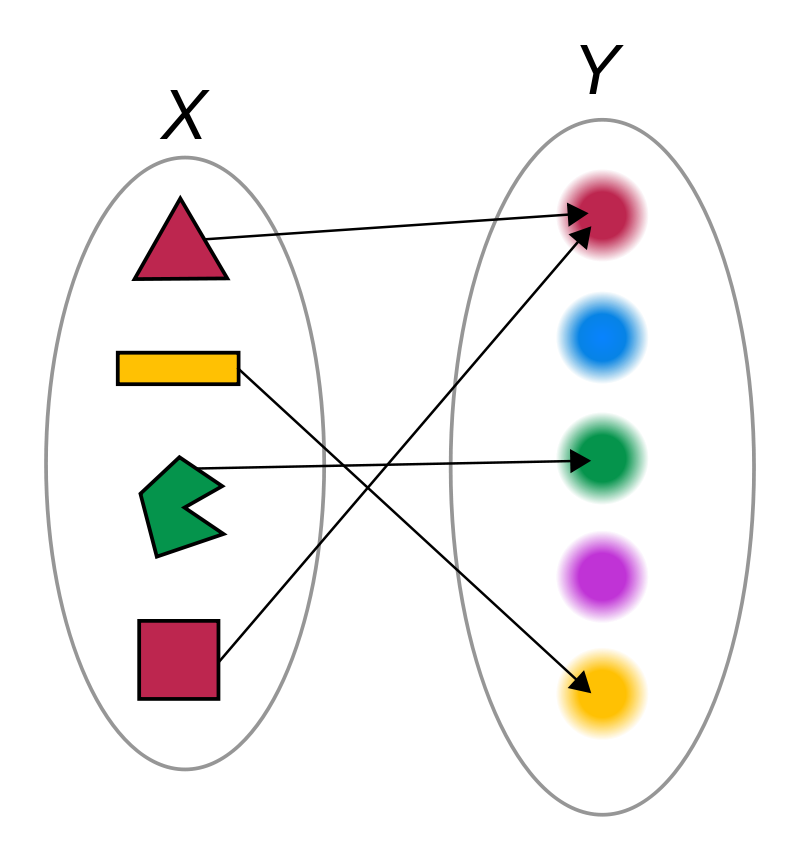
\includegraphics[width = 5cm]{figures/functions/fig-functions-01-00.png}
    \caption{Mapeamento entre o Domínio X e o Domínio Y, ambos não numéricos.}
    \label{fig:functions-01-00}
\end{figure}

\section{Primeiras Definições}


\begin{definition}
    \label{def1}
    Seja um conjunto $A$. A função identidade de $A$ é a função
    $i_A : A \rightarrow A$ definida para todos os valores $x \in A$ tal que $i_A(x) = x$.
\end{definition}

\begin{definition}
    \label{def2}
    Sejam $f : X \rightarrow Y$ e $g : Y \rightarrow Z$ funções.
    Defina $k : X \rightarrow Z$ por $k(x) = g(f(x))$. A função $k$ é chamada de composição
    de $f$ e $g$ ou $f$ composta com $g$ e é escrita $g \circ f$. Desta forma, para cada elemento,
    primeiro  avaliamos $f(x) \in Y$ e depois avaliamos $g(f(x)) \in Z$.
\end{definition}

Podemos ver em Lean as definições de composição e de identidade. Note que estamos em um namespace
hidden para que não haja conflito de definições.

\begin{lstlisting}
namespace hidden
    variables {X Y Z : Type}

    def comp (f : Y → Z) (g : X → Y) : X → Z :=
    λx, f (g x)

    infixr  ` ∘ ` := comp

    #check @comp

    def id (x : X) : X := x

    #check @id

end hidden
\end{lstlisting}

\begin{definition}
    \label{def3}
    Considere $f,g : X \to Y$. Dizemos que essas funções são iguais,
    quando para todos os valores do domínio $X$, a correspondência no contradomínio $Y$ é a
    mesma. Em lógica simbólica, $\forall x (x \in X \to (f(x) = g(x)) \iff f = g $.
\end{definition}

Obseve que em termos de lógica formal de tipos, poderíamos reescrever como
$\forall x : X (f(x) = g(x)) \iff f = g$. Escrevemos essa equivalência entre lógica e funções
utilizando a extensionalidade das funções, muito semelhante à descrita no capítulo de
\textit{\hyperlink{chapter.5}{conjuntos}}. Por exemplo, se $f, g : \mathbb{R} \to \mathbb{R}$
definidas por $f(x) = x + 1$ e $g(x) = 1 + x$, então $f = g$, pois para cada valor de $x$, vale
a comutativade da soma.

Em lean, o comando \lstinline{funext} (de "function extensionality") prova a igualdade de funções.

\begin{lstlisting}
variables {X Y : Type}

example (f g : X → Y) (h : ∀ x, f x = g x) : f = g :=
    funext h
\end{lstlisting}

\begin{theorem}
    \label{prop1}
    Para todo $f: X \to Y$, $f \circ i_X = f$ e $i_Y \circ f = f$
\end{theorem}
\begin{proof}
    Seja $x$ um elemento qualquer de $X$. Então $(f \circ i_X)(x) = f(i_X(x)) = f(x)$
     e $(i_Y \circ f)(x) = i_Y(f(x)) = f(x)$, o que mostra a igualdade.
\end{proof}

No Lean, podemos mostrar essa proposição da seguinte forma. Para algumas funções, será necessário
escrevermos \lstinline{open function}.

\begin{lstlisting}
variables {X Y Z W : Type}

lemma left_id (f : X → Y) : id ∘ f = f := rfl

lemma right_id (f : X → Y) : f ∘ id = f := rfl

theorem comp.assoc (f : Z → W) (g : Y → Z) (h : X → Y) :
    (f ∘ g) ∘ h = f ∘ (g ∘ h) := rfl

\end{lstlisting}

\begin{definition}
    \label{def4}
    Suponha $f:X \to Y$ e $g : Y \to X$ satisfaz $g \circ f = i_X$. Assim,
    $g(f(x)) = i_X(x) = x$, para todos os elementos de $X$. Neste caso $g$ é dita inversa à esquerda
    de $f$ e $f$ é dita inversa à direita de $g$. Quando $g$ é inversa à direita e é inversa à esquerda
    de $f$, então $g$ é dita simplesmente inversa de $f$.
\end{definition}

\begin{example}
    \label{ex1}
    Defina $f,g : \mathbb{R} \to \mathbb{R}$ por $f(x) = x + 1$ e $g(x) = x - 1$. Então $g$
    é inversa à direita e à esquerda de $f$ e vice-versa.
\end{example}
\begin{example}
    \label{ex2}
    $\mathbb{R}^{+}$ denota os reais não negativos. Defina $f : \mathbb{R} \to \mathbb{R}^{+}$
    por $f(x) = x^2$ e defina $g : \mathbb{R}^2 \to \mathbb{R}$ por $g(x) = \sqrt{x}$. Então
    $f(g(x)) = (\sqrt{x})^2 = x$, para todo $x$ no domínio de $g$. Então $f$ é inversa à esquerda de $g$
    e $g$ inversa à direita de $f$. Por outro lado, $g(f(x)) = \sqrt{x^2} = |x|$. Logo $g$ não é inversa à
    esquerda de $f$ e $f$ não é inversa à direita de $g$.
\end{example}

\begin{theorem}
    \label{prop2}
    Suponha que $f : X \to Y $ tem inversa à esquerda, $h : Y \to X $ e uma inversa à direita, $k : Y \to X $.
    Então $h = k$.
\end{theorem}
\begin{proof}
    Seja $y \in Y$. $h(f(k(y))) = k(y)$, pois $h$ é uma inversa à esquerda de $f$.
    Por outro lado, $f(k(y)) = y$ e, portanto $h(f(k(y))) = h(y)$. Assim $k(y) = h(y) $ e as funções são iguais.
\end{proof}

Essa proposição pode também ser vista em Lean. Considerarei a prova utilizando táticas. O leitor pode estudar
aquela que sentir mais confortável. Note que neste exemplo, já foi necessário o \lstinline{namespace function},
visto que \lstinline{left_inverse} e \lstinline{right_inverse} já estão predefinidas.

\begin{lstlisting}
open function

variables {X Y Z: Type}

-- Term and Calc Mode
example (f: X → Y) (h: Y → X) (k: Y → X)
    (hf: left_inverse h f) (fk: right_inverse k f): h = k :=
    have H: ∀ ( x : Y ), h x = k x, from
        assume x,
        have h1: h (f (k x)) = k x , from calc
            h ( f (k x)) = k x: by apply hf,
        have h2: h (f (k x)) = h x, from calc
            h (f (k x)) = h x: by rw fk,
        show h x = k x, from eq.trans (eq.symm h2) h1,
    show h = k, from funext H

-- Tatics Mode
example (f: X → Y) (h: Y → X) (k: Y → X)
    (hf: left_inverse h f) (fk: right_inverse k f): h = k :=
    begin
        apply funext,
        assume x,
        have hf: h (f (k x)) = k x, by apply hf,
        rw ←hf,
        rw fk,
    end
\end{lstlisting}

\begin{theorem}
    \label{prop3}
    Seja $f: X \to Y$. Se a inversa de $f$ existe, então ela é única. Isto é, se $g_1, g_2: Y \to X$ são inversas
    de $f$, então $g_1 = g_2$
\end{theorem}
\begin{proof}
    Sabemos que $g_1$ é inversa à esquerda de $f$. Então,
    $$g_1(f(g_2(x))) = g_2(x), ~para~todos~os~valores~de~x.$$
    Também, $g_2$ é inversa de $f$. Então,
    $$g_1(f(g_2(x))) = g_1(x), ~para~todos~os~valores~de~x.$$ Logo $g_1 = g_2$.
\end{proof}

Quando a inversa de $f$ existe, então, podemos escrevê-la como $f^{-1}$. Dada a Definição \hyperlink{def4},
podemos afirmar que $(f^{-1})^{-1} = f$.

Observe que uma função pode possuir mais de uma função inversa à esquerda ou mais de uma função inversa
à direita. Ainda, quando uma função possui mais de uma função inversa à esquerda, ela não possui inversa
à direita. Se ela possuisse, ela seria igual a todas as funções inversas à esquerda pela Proposição \ref{prop2},
portanto elas seriam iguais, o que é uma contradição, por hipótese. O mesmo vale para inversas à direita.

\begin{theorem}
     \label{prop4}
     Seja $f: X \to Y $ e $g: Y \to Z$. Se $h: Y \to X$ e $k: Z \to Y$ são inversas à esqueda de $f$ e $g$,
     respectivamente, então $h \circ k$ é inversa à esquerda de $g \circ f$. O mesmo vale quando substituimos
     esquerda por direita na proposição.
\end{theorem}

\begin{proof}
 $(h \circ k)\circ(g \circ f)(x) = h(k(g(f(x)))) = h(f(x)) = x $. A demonstração quando substituimos a proposição
 de esquerda para direita é análoga e é deixada como exercício ao leitor.
\end{proof}

\begin{corollary}
    \label{cor1}
    Se $f: X \to Y$ e $g: Y \to Z$ possuem inversas, então $(f \circ g)^{-1}$ existe e
    $(f \circ g)^{-1} = f^{-1} \circ g^{-1}$.
\end{corollary}

\begin{proof}
    Segue diretamente da Proposição \ref{prop4} e Proposição \ref{prop2}.
\end{proof}

\section{Funções Injetiva, Sobrejetiva e Bijetiva}

\begin{definition}[Função Injetiva]
    \label{def5}
    Também conhecida como função injetora, é uma função em que elementos
    distintos do domínio são mapeados para elementos diferentes do
    contradomínio. Dessa forma, seja $f: X \to Y$. Se $\forall x_1 \in X,
    \forall x_2 \in X, x_1 \neq x_2 \Rightarrow f(x_1) \neq f(x_2) $, f é
    injetiva. A definição pode ser feita pela contrapositiva dessa afirmação,
    também. A definição pela contrapositiva será bastante utilizada nas
    demonstrações.
\end{definition}

\begin{definition}[Função Sobrejetiva]
    \label{def6}
    Também conhecida como função bijetora, é uma função em que todos os
    elementos do contradomínio estão na imagem da função. Dessa forma, seja
    $f: X \to Y$. Se $\forall y \in Y, \exists x \in X, f(x) = y$, f é
    sobrejetiva.
   \end{definition}

\begin{definition}[Função Bijetiva]
    \label{def7}
    Também conhecida como bijeção ou correspondência um a um, é uma função
    simultaneamente injetiva e sobrejetiva.
\end{definition}

Em Lean, essas definições são descritas no \lstinline{namespace function}.

\begin{example}
    Considere os conjuntos $X = \{1,2,3,4\}$, numéricos e $Y = \{John, Paul,
    George, Ringo\}$, não numérico.É possível construir uma função
    bijetiva entre $X$ e $Y$. Ainda mais, toda função sobrejetiva entre esses
    conjuntos é também injetiva e consequentemente bijetiva.
\end{example}

\begin{lstlisting}
variables {X Y: Type}

def injective (f : X → Y) : Prop :=
∀ x₁ x₂, f x₁ = f x₂ → x₁ = x₂

def surjective (f : X → Y) : Prop :=
∀ y, ∃ x, f x = y

def bijective (f : X → Y) := injective f ∧ surjective f
\end{lstlisting}

\begin{theorem}
    \label{prop5}
    Seja $f : X \to Y$.
    \renewcommand{\labelenumi}{\Roman{enumi}}
    \begin{enumerate}
        \item Se $f$ possui inversa à esquerda, $f$ é injetiva.
        \item Se $f$ possui inversa à direita, $f$ é sobrejetiva.
        \item Se $f$ possui inversa, $f$ é bijetiva.
    \end{enumerate}
\end{theorem}
\begin{proof}
    Para provar I), suponha que $f(x_1) = f(x_2)$ e que $g$ é inversa à
    esquerda de $f$. Assim $g(f(x_1)) = x_1$ e $g(f(x_2)) = x_2$. Portanto
    $x_1 = x_2$ e está provado. Para provar II), considere $h$ inversa à
    direita de $f$. Seja $y \in Y$ e $x = h(y)$. Então $f(x) = f(h(y)) = y$. A
    terceira sai diretemente das duas anteriores e da Proposição \ref{def2}. 
\end{proof}

\begin{lstlisting}
open function

variables {X Y : Type}

theorem inj_of_left_inverse {g : Y → X} {f : X → Y} :
left_inverse g f → injective f :=
    assume h, assume x₁ x₂, assume feq,
    calc x₁ = g (f x₁) : by rw h
        ... = g (f x₂) : by rw feq
        ... = x₂       : by rw h

theorem surj_of_right_inverse {g : Y → X} {f : X → Y} :
right_inverse g f → surjective f :=
    assume h, assume y,
    let  x : X := g y in
    have f x = y, from calc
        f x  = (f (g y))    : rfl
        ... = y            : by rw [h y],
    show ∃ x, f x = y, from exists.intro x this
\end{lstlisting}

\begin{theorem}
    \label{prop6}
    Seja $f: X \to Y$
    \renewcommand{\labelenumi}{\Roman{enumi}}
    \begin{enumerate}
        \item Se $X$ é não vazio e $f$ é injetiva, então $f$ possui inversa à
        esquerda.
        \item Se $f$ é sobrejetiva, então $f$ possui inversa à direita.
        \item Se $X$ é não vazio e $f$ é bijetiva, então $f$ possui inversa.
    \end{enumerate}
\end{theorem}

\begin{proof}
    Seja $\hat{x} \in X$. Defina uma função $g: Y \to X$ com $g(y) = x$, tal
    que $f(x) = y$, se $y$ pertence a imagem de $f$. Caso não pertença, defina
    $g(y) = \hat{x}$. Agora, assuma $x \in X$. Suponha que $g(f(x)) = x'$.
    Essa suposição é válida, pois $f(x) \in Y$. Pela definição de $g$, como
    $f(x)$ pertence a imagem de $f$, então $g(f(x)) = x'$, tal que $f(x') =
    f(x)$. Como $f$ é injetiva, temos que $x = x'$ e $g(f(x)) = x$ e g é
    inversa à esquerda de $f$. 

    Para a segunda afirmação, defina $h: Y \to X$, onde, para cada $y \in Y$,
    escolha um elemento $x \in X$, tal que $f(x) = y$. Note que a
    sobrejetividade garante a existência desse elemento, mas não garante a
    unicidade na escolha. Então $f(h(y)) = f(x) = y$, por definição de $h$.

    A fim de provar a terceira, basta as demonstrações das anteriores e da
    Proposição \ref{def2}. 
\end{proof}

Algumas observações sobre essa demonstração são importantes. Ao definir $g$ na
primeira parte, precisa-se decidir se $x \in X$ existe tal que $f(x) = y$.
Isso pode não ser algoritmicamente feito, logo $g$ poderia não ser computável.
Na construção de $h$, a prova requere que haja uma escolha de valor de $x$
entre os possíveis candidatos. Isto é uma versão do
\href{https://pt.wikipedia.org/wiki/Axioma_da_escolha#Enunciado}{\textit{axioma
da escolha}}. Este axioma foi muito debatido no século XX, mas hoje já é comum
para demonstrações. O paradoxo de Banach-Tarski é um argumento contra o
axioma. Um bom vídeo sobre o assunto pode ser encontrado nesse
\href{https://www.youtube.com/watch?v=s86-Z-CbaHA}{link}.

Utilizando conceitos e resultados da seção anterior, podemos provar a seguinte
proposição.

\begin{theorem}
    Seja $f: X \to Y$ e $g: Y \to Z$.
    \renewcommand{\labelenumi}{\Roman{enumi}}
    \begin{enumerate}
        \item Se $f$ e $g$ são injetivas, $g \circ f$ também será.
        \item Se $f$ e $g$ são sobrejetivas, $g \circ f$ também será.
    \end{enumerate}
\end{theorem}

\begin{proof}
    Basta aplicarmos a Proposição \ref{def4} e definirmos $h$ e $k$ como
    inversas à esquerda de $f$ e $g$ respectivamente. Logo $(h \circ k)$ é
    inversa à esquerda de  $(g \circ f)$ e, portanto, ela é injetiva.

    O mesmo vale para a segunda afirmação.
\end{proof}

\begin{lstlisting}
open function

namespace hidden
    variables {X Y Z : Type}

    theorem injective_comp {g : Y → Z} {f : X → Y}
    (Hg : injective g) (Hf : injective f) :
    injective (g ∘ f) :=
        assume x₁ x₂,
        assume : (g ∘ f) x₁ = (g ∘ f) x₂,
        have f x₁ = f x₂, from Hg this,
        show x₁ = x₂, from Hf this

    theorem surjective_comp {g : Y → Z} {f : X → Y}
        (hg : surjective g) (hf : surjective f) :
    surjective (g ∘ f) :=
    begin
        assume z,
        apply exists.elim (hg z),
        assume y (hy: g y = z),
        apply exists.elim (hf y),
        assume x (hx: f x = y),
        rw ←hx at hy,
        apply exists.intro x hy
    end

    theorem bijective_comp {g : Y → Z} {f : X → Y}
        (hg : bijective g) (hf : bijective f) :
        bijective (g ∘ f) :=
    have ginj : injective g, from hg.left,
    have gsurj : surjective g, from hg.right,
    have finj : injective f, from hf.left,
    have fsurj : surjective f, from hf.right,
    and.intro (injective_comp ginj finj)
                (surjective_comp gsurj fsurj)
end hidden
\end{lstlisting}

\begin{example}
    Considere $f: \mathbb{N} \to Y$, tal que $f(n) = 2n$. Podemos, ter:
    \begin{itemize}
        \item $Y = \mathbb{N}$. $f$ é injetiva, mas não é sobrejetiva.
        \item $Y = \mathbb{R}$. $f$ é injetiva, mas não é sobrejetiva.
        \item $Y = \{n \in \mathbb{N} | n~par\}$. $f$ é bijetiva.
    \end{itemize}
\end{example}

\section{Funções e Subconjuntos do Domínio}

Nós podemos querer saber o comportamento de uma função em algum subconjunto
$A$ de  $X$. Por exemplo, podemos dizer que $f$ é injetiva em $A$ se para todo
$x_1$ e $x_2$ em A, $f(x_1) = f(x_2) $ implicar $x_1 = x_2 $, por exemplo. A
diferença com relação à função parcial é que nesse caso, a função pode ser
definida em seu complementar. 

\begin{definition}
    \label{def8}
    Se $f$ é função de $X$ e $Y$, dizemos que $f[A]$ denota a imagem de $f$ em
    $A$, definido por $f[A] = \{y \in Y | ~\exists x \in A, y = f(x)\}$.
\end{definition}

\begin{theorem}
    \label{prop7}
    Seja $f: X \to Y $ e $A$ um subconjunto de $X$. Então, para todo $x$ em
    $A$, $f(x)$ está em $f[A]$.
\end{theorem}

\begin{proof}
    Por definição, $f(x) \in f[A] $ se, e somente se, existe $x'$ em $A$ tal
    que $f(x') = f(x)$. Isto vale para  $x' = x $.
\end{proof}

Em Lean, utilizando Táticas, esta prova pode ser apresentada da seguinte
forma: 

\begin{lstlisting}
import data.set 
open function

variables {X Y : Type}

example (f: X → Y) (A : set X) (a : X) (h: a ∈ A) : (f a) ∈ f '' A :=
begin 
    apply exists.intro a, 
    exact and.intro h (eq.refl (f a)),  
end   
\end{lstlisting}

\begin{theorem}
    \label{prop8}
    Seja $f: X \to Y$ e $g: Y \to Z$. Seja $A$ subconjunto de $X$. Então
    $$(g \circ f)[A] = g[f[A]]$$
\end{theorem}

\begin{proof}
    Seja $z \in (g \circ f)[A]$. Então, para algum $x \in A$, $z = (g \circ
    f)(x) = g(f(x))$. Pelo que acabamos de provar na Proposição \ref{prop8},
    $f(x) \in f[A]$. Novamente, pelo que acabamos de provar, $g(f(x)) \in
    g[f[A]] $.

    Alternativamente, seja $z \in g[f[A]]$. Então, existe $y$ em $f[A]$ tal
    que $f(y) = z$. Como $y \in f[A]$, existe $x \in A$, tal que $f(x) = y$.
    Então $(g \circ f)(x) = g(f(x)) = g(y) = z$, então $z \in (g \circ f)[A] $
\end{proof}

Uma prova de que a composição de funções sobrejetivas é sobrejetiva é a que
descrevemos cima, pois $f: X \to Y$ é sobrejetiva se, e somente se, $f[X] =
Y$.

Nós podemos ver $f$ como uma função de $A$, um subconjunto de $X$ a $Y$,
simplesmente ignorando o comportamento de $f$ nos elementos fora de $A$.

\begin{definition}
    \label{def9}
    Denotamos $f \upharpoonright A$ como restrição de $f$ para $A$. Isto é,
    dadas $f: X \to Y$ e $A \subseteq X$, $f \upharpoonright A : A \to Y$ é
    definida por $(f \upharpoonright A)(x) = x$, para todo $x$ em $A$.
\end{definition}

Agora, $f$ é injetiva em $A$ significa que a restrição de $f$ em $A$ é
injetiva.

\begin{definition}[Pré-imagem]
    \label{def10}
    Se $f: X \to Y$ e $B \subseteq Y$, então a pré-imagem de $B$ em $f$,
    denotado por $f^{-1}[B]$ é definida por $f^{-1}[B] = \{x \in X | f(x) \in
    B\}$. Ou seja, é o conjunto de elementos de $X$ que são mapeados em $B$.
\end{definition}

Note que essa definição faz sentido mesmo que $f$ não tenha inversa, visto que
dado $y \in B$ pode não haver $x \in X$ com a propriedade de $f(x) \in B$,
como podem ter vários. Se $f$ tem inversa ($f^{-1}$), então, para todo $y$ em
$B$, existe exatamente um elemento $x$ em $X$ com $f(x) \in B$. Neste caso,
dizemos que $f^{-1}[B]$ é a imagem de $B$ sobre $f^{-1}$ ou a pré-imagem de
$B$ sobre $f$.

Em Lean, a definição de Pré-imagem encontra-se na bilbioteca \textit{Mathlib}
e é definida da seguinte forma: 

\begin{lstlisting}
variables {X Y : Type}

def preimage (f : X → Y) (B : set Y) : set X := {x : X | f(x) ∈ B}

infix ` ⁻¹' `:80 := preimage
\end{lstlisting}


\begin{theorem}
    Seja $f: X \to Y$, $g: Y \to Z$ e $C \subseteq Z$. Então $$(g \circ
    f)^{-1}[C] = f^{-1}[g^{-1}[C]]$$.
\end{theorem}
\begin{proof}
    Para qualquer $y$, $y \in (g \circ f)^{-1}[C]$ se, e somente se, $g(f(y))$
    está em $C$. Isto acontece se, e somente se, $f(y) \in g^{-1}[C]$, o que
    acontece se, e somente se $y \in f^{-1}[g^{-1}[C]]$.
\end{proof}

Seguem algumas propriedades sobre imagens e pré-imagens. Aqui, $f$ denota uma
função arbitrária de $X$ em $Y$. $A, A_1, A_2, ...$ denotam subconjuntos
arbitrários de $X$, e $B, B_1, B_2,...$ denotam subconjuntos arbitrários de
$Y$.

\begin{enumerate}
    \item $A \subseteq f^{-1}[f[A]]$, e se $f$ é injetiva, $A = f^{-1}[f[A]]$.
    \item $f[f^{-1}[B]] \subseteq B$, e se $f$ é sobrejetiva, $B =
    f[f^{-1}[B]]$.
    \item Se $A_1 \subseteq A_2$, então $f[A_1] \subseteq f[A_2]$.
    \item Se $B_1 \subseteq B_2$, então $f^{-1}[B_1] \subseteq f^{-1}[B_2]$.
    \item $f[A_1 \cup A_2] = f[A_1] \cup f[A_2]$.
    \item $f^{-1}[B_1 \cup B_2] = f^{-1}[B_1] \cup f^{-1}[B_2]$.
    \item $f[A_1 \cap A_2] \subseteq f[A_1] \cap f[A_2]$ e, se $f$ é injetiva,
    $f[A_1 \cap A_2] = f[A_1] \cap f[A_2]$.
    \item $f^{-1}[B_1 \cap B_2] = f^{-1}[B_1] \cap f^{-1}[B_2]$.
    \item $f[A] \setminus f[B] \subseteq f[A\setminus B]$.
    \item $f^{-1}[A] \setminus f^{-1}[B] \subseteq f[A \setminus B]$.
    \item $f[A] \cap B = f[A \cap f^{-1}[B]]$.
    \item $f[A \cup f^{-1}[B]] \subset f[A] \cup B $.
    \item $A \cap f^{-1}[B] \subseteq f^{-1}[f[A] \cap B]$.
    \item $A \cup f^{-1}[B] \subseteq f^{-1}[f[A] \cup B]$.
\end{enumerate}

A partir de agora, vamos demonstrar algumas dessas proporições, ora com
descrições da demonstração e ora com provas em Lean. Tambémm sugerimos que
essas proposições sejam exercícios para a leitora ou o leitor.

\subsection{Demonstrações com linguagem natural}

\begin{theorem}[Item 7]
    \label{exerc1}
    Sejam $X$ e $Y$ conjuntos, $A_1, A_2 \in X$ e $f: X \to Y$.
\end{theorem}

\begin{proof}
    Se $y \in f[A_1 \cap A_2]$, temos que existe $x \in A_1 \cap A_2$, com
    $f(x) = y$. Nesse caso, $f(x) \in f[A_1]$, e $f(x) \in f[A_2]$, o que
    demonstra a primeira parte.

    Agora, suponha a injetividade de $f$. Suponha também que $y \in f[A_1]
    \cap f[A_2]$. Assim, existem $x_1 \in A_1$ e $x_2 \in A_2$, com as
    propriedades de $f(x_1) = y = f(x_2)$. Como a função é injetiva, $f(x_1) =
    f(x_2) \Rightarrow x_1 = x_2$. Assim $x_1 \in A_2$, que implica $x_1 \in
    A_1 \cap A_2$. Logo, $y \in f[A_1 \cap A_2]$.
\end{proof}

\begin{theorem}[Item 11]
    \label{exerc2}
    Sejam $X$ e $Y$ conjuntos, $f: X \to Y, A \subseteq X$ e $B \subseteq Y$.
    Então, $f[A] \cap B = f[A \cap f^{-1}[B]]$
\end{theorem}

\begin{proof}
    Suponha, inicialmente, que $y \in f[A] \cap B$. Então $y \in B$ e para
    algum $x \in A$, $f(x) = y$. Nesse sentido, $x \in f^{-1}[B]$. Assim, $x
    \in A \cap f^{-1}[B]$ e, portanto, $y \in f[A \cap f^{-1}[B]]$.

    Alternativamente, se $y \in f[A \cap f^{-1}[B]]$, existe $x \in A \cap
    f^{-1}[B]$, com $f(x) = y$. Daqui, concluímos que $y = f(x) \in f[A]$ e $y
    \in B$, pela definição de pré-imagem. Então $y \in f[A] \cap B$, como
    queríamos provar.
\end{proof}

\begin{theorem}[Item 13]
\end{theorem}

\begin{proof}
    Suponha que $x \in A \and f^{-1}[B]$. Desta maneire, $x \in A$ e $x \in
    f^{-1}[B]$, que implica que existe $y \in B$, tal que $f(x) = y$. Nesse
    sentido, $y \in B$ e $y \in f[A]$, que implica $y \in f[A] \and B$. Como
    $f(x) = y $, então $x \in f^{-1}[f[A]\and B]$. 

\end{proof}

\subsection{Demontrações em Lean}

Nós podemos utilizar variáveis limitadas para falar sobre o comportamento de
funções em conjuntos particulares.

\begin{lstlisting}
import data.set -- inclui o símbolo de subconjunto da imagem ''
open set function

variables {X Y : Type}
variables (A  : set X) (B : set Y)

def maps_to (f : X → Y) (A : set X) (B : set Y) :=
    ∀ x ∈ A, f x ∈ B

def inj_on (f : X → Y) (A : set X) :=
    ∀ (x₁ ∈ A) (x₂ ∈ A), f x₁ = f x₂ → x₁ = x₂

def surj_on (f : X → Y) (A : set X) (B : set Y) :=
    B ⊆ f '' A

\end{lstlisting}

A definição de \lstinline{maps_on} é a ideia de que a imagem de um subconjunto
do domínio $X$ está totamente inclusa em um subconjunto específico do
contradomínio. As definições de \lstinline{inj_on} e \lstinline{surj_on} são
as definições usuais.

\begin{theorem}[Item 1]
\end{theorem}

\begin{lstlisting}
import data.set 
open function
open set 

variables {X Y : Type}

theorem item1.a (f : X → Y) (A : set X) : A ⊆  f ⁻¹' (f '' A) := 
assume a h, 
have h1: a ∈ A ∧ f a = f a, from and.intro h (eq.refl (f a)),
have h2: (f a) ∈ f '' A, from exists.intro a h1,   
show a ∈ f ⁻¹' (f '' A), from h2

theorem item1.b (f : X → Y) (A : set X) (h: injective f): 
        A =  f ⁻¹' (f '' A) :=
eq_of_subset_of_subset
(item1.a f A)
(assume x h1, 
have h2: f x ∈ f '' A, from h1,
have h3: ∃ (a : X), a ∈ A ∧ f a = f x, from h1,
show x ∈ A, from exists.elim h3
    (assume (y : X) (h4: y ∈ A ∧ f y = f x),
    have h5: y = x, from h h4.right,
    show x ∈ A, from eq.subst h5 h4.left)
)
\end{lstlisting}

\begin{theorem}[Item 3]
\end{theorem}

\begin{lstlisting}
import data.set
open set function

variables {X Y : Type}
variables (A B A₁ A₂ : set X)

theorem item3 (f: X → Y) : A₁ ⊆ A₂ → f '' A₁ ⊆ f '' A₂ :=
    assume h : A₁ ⊆ A₂,
    assume y,
    assume h₁ : y ∈ f '' A₁,
    have h₂ : ∃ x, x ∈ A₁ ∧ f(x) = y, from h₁,
    show y ∈ f '' A₂, from exists.elim h₂
        (assume (x' : X) (ha: x' ∈ A₁ ∧ f(x') = y ),
        have h₃ : x' ∈ A₂ ∧ f(x') = y, from and.intro (h ha.left)  ha.right,
        show y ∈ f '' A₂, from exists.intro x' h₃)    
\end{lstlisting}

\begin{theorem}[Item 9]
\end{theorem}

Observe que para o item 9, trataremos $X$ e $Y$ como conjuntos iguais. Caso
não sejam, $f[B]$ pode nem estar definida.

\begin{lstlisting}
import data.set
open set function

variables {X Y : Type}
variables (A B A₁ A₂ : set X)

theorem item9 (f: X → X) : f '' A \ f '' B ⊆ f '' (A \ B) :=
begin
    intros y h,
    have h₁ : y ∈ f '' A, from mem_of_mem_diff h,
    have h₂ : ¬ (y ∈ f '' B), from not_mem_of_mem_diff h,
    apply exists.elim h₁,
    intros x h₃,
    apply exists.intro x,
    apply and.intro,
    apply mem_diff_of_mem,
        exact h₃.left,
        assume h₄ : x ∈ B,
        exact false.elim (h₂ (exists.intro x (and.intro h₄ h₃.right))),
        exact h₃.right
end

#check @mem_of_mem_diff
#check @not_mem_of_mem_diff
#check @mem_diff_of_mem

\end{lstlisting}

As funções \lstinline{mem_of_mem_diff, not_mem_of_mem_diff} e
\lstinline{mem_diff_of_mem} tem o objetivo de lidar com a diferença e sua
relação com a interseção. Note que usar táticas auxilia o passo a passo, porém
dificulta o posterior entendimento. Por isso, é recomendável, nesses exemplos,
utilizar alguma ferramenta para Lean. Essas funções e outras já apresentadas,
encontram-se na biblioteca do Lean e grande parte delas está disponível quando
você abre o namespace \lstinline{function}.

\begin{lstlisting}
open function 

#check @comp 
#check @has_left_inverse
-- A right_inverse tem duas definicoes para Lean. Apenas uma
-- esta no namespace function. Por isso e importante especificar. 
#check @function.right_inverse    
\end{lstlisting}

\subsection{Definindo a inversa Classicamente}

Para definir funções inversas, é necessário que utilizemos o racionínio
clássico. 

\begin{lstlisting}
open classical 

#check @axiom_of_choice
#check @some_spec

variables A B : Type
variable P : A → Prop   
variable R : A → B → Prop

example : (∀ x, ∃ y, R x y) → ∃ f : A → B, ∀ x, R x (f x) :=
axiom_of_choice

example (h : ∃ x, P x) : P (some h) :=
some_spec h    
\end{lstlisting}

O axioma da escolha fala que se para todo \lstinline{x : X}, existe
\lstinline{y: Y} com \lstinline{R x y}, então existe uma função \lstinline{f: X → Y} que para todo \lstinline{x}, escolhe-se \lstinline{y}. Em Lean, é
utilizada a função \lstinline{some} para mostrar este axioma, através da
construção clássica. Podemos, portanto, definir a inversa como: 

\begin{lstlisting}
open classical function
local attribute [instance] prop_decidable

variables {X Y : Type}

noncomputable def inverse (f : X → Y) (default : X) : Y → X :=
λ y, if h : ∃ x, f x = y then some h else default   
\end{lstlisting}

Observe que a definição é não computacional, visto que como já argumentamos,
para uma determinada função, essa hipótese \lstinline{h} pode não ser possível
de validar algoritmicamente e, se a hipótese for válida, pode não ser possível
encontrar um valor de \lstinline{x} adequado, também algoritmicamente. Também
observe que essa inversa é definida assumindo \lstinline{y}, logo ela é
definida para todo valor que ele assume e retorna algum valor qye cumpre essa
propriedade \lstinline{f x = y}, quando a hipótese é válida, ou um valor
padrão dado inicialmente, caso não exista. O comando \lstinline{local attribute} 
fala para a instância que a regra \lstinline{prop_decidable} vai
ser utilizada no arquivo que se segue. Nesse caso, importamos os axiomas
clássicos e tornamos disponível a instância genérica da decição.   

Podemos, então, demonstrar os seguintes teoremas. 

\begin{lstlisting}
open classical function
local attribute [instance] prop_decidable

variables {X Y : Type}

noncomputable def inverse (f : X → Y) (default : X) : Y → X :=
λ y, if h : ∃ x, f x = y then some h else default

theorem inverse_of_exists (f : X → Y) (default : X) (y : Y)
    (h : ∃ x, f x = y) : f (inverse f default y) = y :=
    have h₁ : inverse f default y = some h, from dif_pos h,
    have h₂ : f (some h) = y, from some_spec h,
eq.subst (eq.symm h₁) h₂

#check @dite
#check @dif_pos 

-- Using Term Mode 
theorem is_left_inverse_of_injective (f : X → Y) (default : X)
    (injf : injective f) : left_inverse (inverse f default) f :=
let finv := (inverse f default) in
    assume x,
    have h1 : ∃ x', f x' = f x, from exists.intro x rfl,
    have h2 : f (finv (f x)) = f x, 
        from inverse_of_exists f default (f x) h1,
    show finv (f x) = x, from injf h2

-- Using Tatic Mode 
theorem is_left_inverse_of_injective2 (f : X → Y) (default : X)
    (injf : injective f) : left_inverse (inverse f default) f :=
begin 
    intro x,
    apply injf, 
    apply inverse_of_exists,
    apply exists.intro x,
    exact eq.refl (f x), 
end
\end{lstlisting}

Observado o significado de \lstinline{dite}, que expressa a validade de um
\lstinline{α : Sort}, independente de \lstinline{c: Prop} e o significado de
\lstinline{dif_pos}, que expressa a igualdade entre uma expressão do formato
\lstinline{dite} e outra do mesmo \lstinline{Sort}, podemos entender o
siginificado dessa prova. A versão em Táticas foi inserida como instrução de
aplicação em comparação como o modo em termos. 

\section{Lógica de Segunda ou Mais Alta Ordem}

Até agora, formalmente, definimos lógica de primeira ordem, onde iniciamoscom um estoque 
fixo de símbolos de funções e relações, nos últimos tópicos que  consideramos, ocorre a motivação 
de extender a linguagem para funções e relações. Por exemplo, ao afirmar que $f: X \to Y$ possui 
inversa a esquerda pode ser dito como: $$\exists g, \forall x, g(f(x)) = x.$$
Outro exemplo é o seguinte teorema, descrito em linguagem lógica 
$$\forall x_1, x_2, (f(x_1) = f(x_2) \to x_1 = x_2) \to \exists g, \forall x, g(f(x)) = x.$$
Isto é, se $f: X \to Y$ é injetiva, então existe inversa à sua esquerda.

Nesse sentido, existe uma quantificação sobre as funções e relações, o que se distancia do que a lógica 
de primeira ordem cobre. Como forma de resolver esse impasse, podemos desenvolver uma teoria na linguagem 
de lógica de primeira ordem no qual o universo contém funções e relações como objetos ou extender essa linguagem
para envolver novos tipos de quantificadores e variáveis, que é o caso descrito nessa sessão. Isto é o que Lógica
de Ordem mais Alta faz. 

Alonzo Church (1903 - 1995) foi um matemático e lógico estadunidense, conhecido pelo cálculo lambda, formulou a ideia
de ordens mais altas na lógica. Isso é algumas vezes descrito como Teoria Simples dos Tipos ou Teoria dos Tipos de 
Chunch's. Sejam $X, Y, Z,...$ tipos básicos e $Prop$ um tipo especial das proposições. Temos, então:
\begin{itemize}
    \item Se $X$ e $Y$ são tipos, então $U \times V$ também será.Isto denota que o par ordenado $(x,y)$, com $x \in X$ 
    e $y \in Y$ é tipado. 
    \item Se $X$ e $Y$ são tipos, então $U \to V$ também será.
\end{itemize}

Para formar expressões, a teoria de Church aficiona os seguintes caminhos: 
\begin{enumerate}
    \item Se $x$ é do tipo $X$ e $y$ é do tipo $Y$, $(x,y)$ é do tipo $X \times Y$. 
    \item Se $z$ é do tipo $X \times Y$, então $(p)_1$ é do tipo $X$ e $(p)_2$ é do tipo $Y$, que denotam o primeiro e 
    segundo elemento do par $z$, respectivamente. 
    \item Se $x$ é uma variável do tipo $X$ e $y$ é uma expressão do tipo $Y$, então $\lambda x y$ é do tipo $X \to Y$. 
    Para lembrar o significado dessa expressão, voltar em \ref{concept}.
    \item Se $f$ é do tipo $X \to Y$ e $x$ é do tipo $X$, $f(x)$ é do tipo $Y$. 
\end{enumerate}

Além desses meios, a teoria simples dos tipos possui conetivos booleanos, quantificadores e a igualdade, oriunda da lógica
de primeira ordem, para construir proposições. 

A fução $f(x,y)$ que toma elementos de $X$ e $Y$ para o tipo $Z$ é vista como um objeto do tipo $X \times Y \to Z$. Note que,
nesse sentido, uma relação binária $R(x,y)$ definida em $X$ e $Y$ é vista como um objeto $X \times Y \to Prop$. O que torma essa 
lógica ser de ordem mais alta é que podemos iterar o tipo função indefinidamente. Por exemplo, se $\mathbb{N}$ é o tipo dos números
naturais, $\mathbb{N} \to \mathbb{N}$ denota o tipo das funções dos números naturais aos números naturais, e $(\mathbb{N} \to \mathbb{N}) \to \mathbb{N}$ 
denota o tipo de funções $F(f)$ que tomam uma função como argumento e retornam um número natural. Vamos ver em Lean:

\begin{lstlisting}
open nat 

#check ℕ                -- ℕ : Type
#check ℕ → ℕ            -- ℕ → ℕ : Type
#check (ℕ → ℕ) → ℕ      -- (ℕ → ℕ) → ℕ : Type 

variable F: (ℕ → ℕ) → ℕ 
variable f: ℕ → ℕ
variable n: ℕ 

#check f n              -- f n : ℕ 
#check F f              -- F f : ℕ 
#check F n              -- error
\end{lstlisting}

A variavél $F$ espera uma função, por isso retorna erro no último \lstinline{#check}. Se retirarmos o parênteses, Lean entenderá que 
\lstinline{F : ℕ → (ℕ → ℕ)}. 

As especificações de síntaxe e regras da lógica de ordem mais alta são descritas mais cuidadosamente em livros-texto mais avançados. 
Para considerar os tipos de funções e relações, basta o conhecimento de lógica de segunda ordem. É importante ter em mente que já lidamos 
desde os primeiros capítulos com os tipos e lógica de segunda ordem, em Lean, que é um sistema de lógica ainda mais elaborado e expressivo. 

\subsection{Definindo a inversa Classicamente}

Para definir funções inversas, é necessário que utilizemos o racionínio clássico. 

\begin{lstlisting}
open classical 

#check @axiom_of_choice
#check @some_spec

variables A B : Type
variable P : A → Prop   
variable R : A → B → Prop

example : (∀ x, ∃ y, R x y) → ∃ f : A → B, ∀ x, R x (f x) :=
axiom_of_choice

example (h : ∃ x, P x) : P (some h) :=
some_spec h    
\end{lstlisting}

O axioma da escolha fala que se para todo \lstinline{x : X}, existe \lstinline{y: Y} com 
\lstinline{R x y}, então existe uma função \lstinline{f: X → Y} que para todo \lstinline{x},
escolhe-se \lstinline{y}. Em Lean, é utilizada a função \lstinline{some} para mostrar este a 
axioma, através da construção clássica. Podemos, portanto, definir a inversa como: 

\begin{lstlisting}
open classical function
local attribute [instance] prop_decidable

variables {X Y : Type}

noncomputable def inverse (f : X → Y) (default : X) : Y → X :=
λ y, if h : ∃ x, f x = y then some h else default   
\end{lstlisting}

Observe que a definição é não computacional, visto que como já argumentamos, para uma determinada função, essa 
hipótese \lstinline{h} pode não ser possível de validar algoritmicamente e, se a hipótese for válida, pode não 
ser possível encontrar um valor de \lstinline{x} adequado, também algoritmicamente. Também observe que essa inversa é 
definida assumindo \lstinline{y}, logo ela é definida para todo valor que ele assume e retorna algum valor qye cumpre 
essa propriedade \lstinline{f x = y}, quando a hipótese é válida, ou um valor padrão dado inicialmente, caso não exista. 
O comando \lstinline{local attribute} fala para a instância que a regra \lstinline{prop_decidable} vai ser utilizada no 
arquivo que se segue. Nesse caso, importamos os axiomas clássicos e tornamos disponível a instância genérica da decição.   

Podemos, então, demonstrar os seguintes teoremas. 

\begin{lstlisting}
open classical function
local attribute [instance] prop_decidable

variables {X Y : Type}

noncomputable def inverse (f : X → Y) (default : X) : Y → X :=
λ y, if h : ∃ x, f x = y then some h else default

theorem inverse_of_exists (f : X → Y) (default : X) (y : Y)
    (h : ∃ x, f x = y) : f (inverse f default y) = y :=
    have h₁ : inverse f default y = some h, from dif_pos h,
    have h₂ : f (some h) = y, from some_spec h,
eq.subst (eq.symm h₁) h₂

#check @dite
#check @dif_pos 

-- Using Term Mode 
theorem is_left_inverse_of_injective (f : X → Y) (default : X)
    (injf : injective f) : left_inverse (inverse f default) f :=
let finv := (inverse f default) in
    assume x,
    have h1 : ∃ x', f x' = f x, from exists.intro x rfl,
    have h2 : f (finv (f x)) = f x, 
        from inverse_of_exists f default (f x) h1,
    show finv (f x) = x, from injf h2

-- Using Tatic Mode 
theorem is_left_inverse_of_injective2 (f : X → Y) (default : X)
    (injf : injective f) : left_inverse (inverse f default) f :=
begin 
    intro x,
    apply injf, 
    apply inverse_of_exists,
    apply exists.intro x,
    exact eq.refl (f x), 
end
\end{lstlisting}

Observado o significado de \lstinline{dite}, que expressa a validade de um 
\lstinline{α : Sort}, independente de \lstinline{c: Prop} e o significado 
de \lstinline{dif_pos}, que expressa a igualdade entre uma expressão do formato 
\lstinline{dite} e outra do mesmo \lstinline{Sort}, podemos entender o siginificado
dessa prova. A versão em Táticas foi inserida como instrução de aplicação em comparação
como o modo em termos. 

\section{Funções e Relações}

Podemos ver que nem toda relação é uma função. Uma relação binária $R(x,y)$ em $A$ e $B$ 
é um \textit{funcional} se para todo $x$ em $A$, existe um valor único $y$ em $B$ tal que 
$R(x,y)$. Se $R$ é uma relação funcional, podemos definir $f_R: X \to B$ fazendo com que 
$f_R(x)$ seja igual ao valor de $y$ único em $B$ em que a relação seja verdadeira. A 
contrapartida é verdadeira, basta definir, para $f: X \to B$, $R_f(x,y)$, uma relação funcional. 
Essa relação é conhecida como o \textit{grafo de f}. 

Podemos extrair dessa ideia que existe uma dualidade entre uma relação funcional $R$ e uma 
função $f$. Inclusive, muitas vezes, as definições são intercambiáveis. Em fundamentos tipo-teóricos, 
como a que vemos em Lean, relações são frequentemente definidas como uma classe de funções, enquanto 
para fundamentos teóricos em conjuntos definem função como uma relação funcional. 

Podemos considerar funções $f(x,y)$ ou $g(x,y,z)$ que tomam múltiplos argumentos. Por exemplo, 
$f(x,y) = x + y$. Em lean, podemos exemplificar da seguinte forma: 

\begin{lstlisting}
variables X Y : Type 
variable f: X → X → X → Y 
variables x₁ x₂ x₃  : X

#check f x₁ x₂ x₃ -- tipo Y

def g (x y : ℤ): ℤ := x + y

example : g 1 1 = 2 := 
calc 
g 1 1 = 1 + 1 : by rw g 
    ... = 2 :  rfl
\end{lstlisting}

O número de argumentos de uma função é chamado de \textit{aridade}, que em inglês é \textit{arity}. 
No exemplo acima $f$ tem aridade $3$, enquanto $g$ tem aridade $2$.
Podemos pensar uma função com múltiplos argumentos como uma função unária definida em um produto cartesiano. 
Nesse sentido, quando estamos nos tratando de teoria dos tipos, é conveniente pensar que $f$ é uma função de $X$
que retorna uma função $X \to X \to Y$. Desta maneira, $f(x_1, x_2, x_3)$ abrevia $((f(x_1))(x_2))(x_3)$.

\begin{example}[Teorema de Cantor]
    \label{cantor}
    Seja $f$ uma função que mapeia elementos do conjunto $A$ para o seu conjunto das partes $P(A)$. Então $f: A \to P(A)$ 
    não é sobrejetiva. 
    Esse teorema é um teorema fundamental sobre conjuntos que foi apresentada nesse capítulo devido às definições importantes
    de funções. A referência é no capítulo sobre \hyperlink{chapter.5}{Conjuntos}. A demonstração se dá por contradição e é realizada
    no Lean com o auxílio do \lstinline{namespace classical}. 

    \begin{lstlisting}
    import data.set

    variables X Y: Type 
    
    def surjective {X: Type} {Y: Type} (f : X → Y) : Prop := ∀ y, ∃ x, f x = y
    
    theorem Cantor : ∀ (A: set X), ¬ ∃ (f: A → set A),  surjective f :=
    
        begin
            intro A,
            intro h,
            -- Utiliza a regra eliminação existe.
            cases h with f h1,
            -- Como f é sobrejetiva e esse é um subconjunto de A            
            have h2: ∃ x, f x = {t : A | ¬ (t ∈ f t)},  
                from h1 {t : A | ¬ (t ∈ f t)},
            -- Eliminação do existe, novamente. 
            cases h2 with x h3,
            -- classical.em A := A ∪ ¬A é uma tautologia. 
            apply or.elim (classical.em 
                          (x ∈ {t : A | ¬ (t ∈ f t)})),
                intro h4,
            -- Usa a proriedade do conjunto
                    have h5: ¬ (x ∈ f x), from h4,
                    rw (eq.symm h3) at h4, 
                    apply h5 h4,
                intro h4,
                    rw (eq.symm h3) at h4,
                    have h5: x ∈ {t : A | ¬ (t ∈ f t)}, from h4,
                    rw (eq.symm h3) at h5,
                    apply h4 h5,                     
        end   
    \end{lstlisting}
\end{example}

\subsection{Representação de Funções}

Apesar de não ser o objetivo nesse capítulo, considere a seguinte definição: 

\begin{definition}
    \label{represent}
    A grosso modo, uma função total $f(x_1, ..., x_k)$ é dita
    \textit{representável}, se existe uma expressão na linguagem formal,
    digamos $A$, que usa variáveis $x_1, ..., x_k, x_{k+1}$ tal que para
    quaisquer números $m_1,...,m_k$ e $n$, temos $f(m_1,...,m_k) = n$ se, e
    somente se, podemos provar em nosso sistema formal $A(m_1,...,m_k,n)$ e
    não podemos provar $A(m_1,...,m_k,j)$ para qualquer outro número $j$.
\end{definition}

Essa definição é encontrada no livro \cite{functionsComputaveis}. Apesar de
estar em termos um pouco diferentes dos que propomos nesse livro, essa
definição permite, em um sistema consistente, afirmar que toda função
representável é computável. Isso responde parcialmente nossa questão da
primeira sessão. Entretanto, em livros mais avançados de lógica, esse conceito
é mais discutido. 

\section{Exercícios}

\begin{enumerate}
    \item Quais das seguintes funções são totais: 
    \begin{enumerate}
        \item $f : \mathbb{N} \to \mathbb{N}$, definida por $f(n) = n - 1$.
        \item $g : \mathbb{R}\setminus\{1\} \to \mathbb{R}$, definida por $g(x)
        = \frac{x}{x - 1}$. 
        \item A função de Heaviside. \href{http://mathworld.wolfram.com/
        HeavisideStepFunction.html}{Referência}. 
        \item $h : \mathbb{R}^+ \to \mathbb{R}$, definida por $h(x) = log(x)$.
    \end{enumerate}
    \item Seja $f : X \to Y$ e $g : Y \to Z$. 
    \begin{enumerate}
        \item Mostre que se $g \circ f$ é uma função injetiva, então $f$ é
        injetiva. 
        \item Mostre um exemplo onde a condição do item anterior ocorra, porém
        $g$ não seja injetiva. 
        \item Prove que se $f$ é sobrejetiva e $g \circ f$ é injetiva, então
        $g$ é injetiva. 
        \item Demonstre (a) e (c) utilizando Lean. 
    \end{enumerate}
    \item Uma função $f : X \to Y$ é dita \textit{monótona} se preserva ou
    inverte a relação de ordem. Se a função é estrita, a relação establecida é
    a de $<$. Isto é, se $\forall x_1, \forall x_2, x_1 < x_2 \Rightarrow
    f(x_1) < f(x_2) $ mostra que $f$ é estritamente crescente e com o sinal
    invertido, $f$ será estritamente decrescente. Prove que toda função
    monótona é injetiva. Defina em Lean e prove esse teorema, considerando $X
    = Y = \mathbb{N} $. 
    \item Prove que a função $g : \mathbb{N} \to \mathbb{N}$ definida por
    $g(n) = \left \lceil{\frac{n}{2}}\right \rceil$ é sobrejetiva. Essa função
    é injetiva? 
    \item Prove os item 5 da lista \ref{iden}. Utilize Lean.
\end{enumerate}

\section{Gabarito}

\begin{enumerate}
    \item b e c. No primeiro caso, a função não é definida para $f(0)$, pois
    esse não tem antecessor. No quarto caso, a função não é definida para
    $h(0)$. 
    \item Seguem as provas: 
    \begin{enumerate}
        \item Sejam $x_1 \in X$ e $x_2 \in X$, com $f(x_1) = f(x_2)$. Como $g$
       é uma função bem definida, $g(f(x_1)) = (g \circ f)(x_1) = (g \circ
       f)(x_2) = g(f(x_2))$. Pela injetividade da composição, $x_1 = x_2$ está
        provado. 
        \item Para essa questão, existem vários exemplos. Seja $f : \mathbb{N}
        \to \mathbb{R} $ definida por $f(n) = n$ e seja $g : \mathbb{R} \to
        \mathbb{R}$, $g(x) = x^2 $. Temos que $(g \circ f) : \mathbb{N} \to
        \mathbb{R}$ é definida por $g(f(n)) = n^2$. Note que essa função é
        injetiva, porém $g$ não é. 
        \item Assuma $y_1, y_2 \in Y$. Se $g(y_1) = g(y_2)$, pela
        sobrejetividade de $f$, existem $x_1, x_2 \in X$, tal que $f(x_1) =
        y_1$ e $f(x_2) = y_2$. Pela injetividade da composição, $x_1 = x_2$.
        Como $f$ é uma função bem definida, $y_1 = f(x_1) = f(x_2) = y_2$, o
        que demostra a injetividade de $g$.
        \item Em lean, 
\begin{lstlisting}
import data.set 
open function
open set 

variables {X Y Z: Type}

theorem e2a (f : X → Y) (g: Y → Z) (h: injective (g ∘ f)) : injective f := 
assume x₁ x₂ h₁,
have h₂ : g(f(x₁)) = g(f(x₂)), from eq.subst h₁ (eq.refl (g(f x₁))), 
show x₁ = x₂, from h h₂

theorem e2c (f : X → Y) (g: Y → Z) (h₁: injective (g ∘ f)) (h₂: surjective f) :
        injective g := 
assume y₁ y₂ g₁, 
have g₂ : ∃ x, f(x) = y₁, from h₂ y₁,
have g₃ : ∃ x, f(x) = y₂, from h₂ y₂,
show y₁ = y₂, from exists.elim g₂ 
    (assume x₁ i₁, 
    show y₁ = y₂, from exists.elim g₃ 
        (assume x₂ i₂, 
        have i₃ : g(f(x₁)) = g(y₁), from eq.subst i₁ (eq.refl (g(f x₁))),
        have i₄ : g(f(x₂)) = g(y₂), from eq.subst i₂ (eq.refl (g(f x₂))),
        have i₅ : x₁ = x₂, from h₁ (eq.trans i₃ (eq.trans g₁ (eq.symm i₄))), 
        have i₆ : f(x₁) = f(x₂), from eq.subst i₅ (eq.refl (f(x₁))),
        show y₁ = y₂, from eq.trans (eq.trans (eq.symm i₁) i₆) i₂))    
\end{lstlisting}
    \end{enumerate}
    \item Seja $f: X \to Y$ monótona. Assuma $x_1, x_2 \in X$ e $f(x_1) =
    f(x_2)$. Se $x_1 < x_2$ ou $x_1 > x_2$, temos um absurdo. Logo $x_1 =
    x_2$, o que mostra que $f$ é monótona. 

    Para lean, eu faço uso de uma função \lstinline{ne_of_lt}, que significa
    que dado uma relação de menor ou maior entre dois naturais, eles são
    diferentes. 

\begin{lstlisting}
open function 

variables {X Y Z: Type}

def strict_cresc (f: ℕ → ℕ) := 
    ∀ x1, ∀ x2, x1 < x2 → f x1 < f x2 

def strict_decresc (f: ℕ → ℕ) := 
    ∀ x1, ∀ x2, x1 < x2 → f x1 > f x2 

def monotonous (f: ℕ → ℕ) : Prop := 
    strict_cresc f ∨ strict_decresc f 

lemma inj_of_cresc (f: ℕ → ℕ) (h: strict_cresc f) : injective f := 
assume x1 x2 h1,
nat.lt_by_cases
    (assume : x1 < x2, 
    have h2: f x1 < f x2, from h x1 x2 this,
    show x1 = x2, from false.elim (ne_of_lt h2 h1))
    (assume : x1 = x2, this)
    (assume : x1 > x2, 
    have h2: f x2 < f x1, from h x2 x1 this, 
    show x1 = x2, from false.elim (ne_of_lt h2 (eq.symm h1)))

lemma inj_of_decresc (f: ℕ → ℕ) (h: strict_decresc f) : injective f := 
assume x1 x2 h1,
nat.lt_by_cases
    (assume : x1 < x2, 
    have h2: f x1 > f x2, from h x1 x2 this,
    show x1 = x2, from false.elim (ne_of_lt h2 (eq.symm h1)))
    (assume : x1 = x2, this)
    (assume : x1 > x2, 
    have h2: f x2 > f x1, from h x2 x1 this, 
    show x1 = x2, from false.elim (ne_of_lt h2 h1))

theorem inf_mon (f: ℕ → ℕ)(h: monotonous f):injective f := 
begin 
    cases h, 
    apply inj_of_cresc f h, 
    apply inj_of_decresc f h
end

#check @ne_of_lt   
\end{lstlisting}

\item Suponha $y \in \mathbb{N}$. Note que posso escrever $2\cdot y = n$. De
fato, $g(n) = \left \lceil \frac{2y}{2} \right \rceil = \left \lceil y \right
\rceil = y $, pois $y$ é natural. Assim $\exists n \in \mathbb{N}, g(n) = y$.
Assim, a função é sobrejetiva. 

\item Considere o item 5 Suponha $y \in f[A_1 \cup A_2]$ Assim, existe $x \in
A_1 \cup A_2 $, tal que $f(x) = y$. Se $x \in A_1$, $f(x) = y \in f[A_1]$ e
análogo se $x \in A_2$. Logo $y \in f[A_1] \cup f[A_2]$. Alternativamente, se
$y \in f[A_1] \cup f[A_2]$. Suponha $y \in f[A_1]$. Então existe $x \in A_1$,
tal que $f(x)= y$ e $x \in A_1 \cup A_2$ que implica $y \in f[A_1 \cup A_2]$.
Análogo para $y \in f[A_2]$.

\begin{lstlisting}
import data.set
open function set

variables {X Y : Type}
variable  f : X → Y
variables A1 A2 : set X

example : f '' (A1 ∪ A2) = f '' A1 ∪ f '' A2 :=
eq_of_subset_of_subsetimport data.set
open function set

variables {X Y : Type}
variable  f : X → Y
variables A1 A2 : set X

example : f '' (A1 ∪ A2) = f '' A1 ∪ f '' A2 :=
eq_of_subset_of_subset
    (assume y,
    assume h1 : y ∈ f '' (A1 ∪ A2),
    exists.elim h1
    (assume x h,
    have h2 : x ∈ A1 ∪ A2, from h.left,
    have h3 : f x = y, from h.right,
    or.elim h2
        (assume h4 : x ∈ A1,
        have h5 : y ∈ f '' A1, from ⟨x, h4, h3⟩,
        show y ∈ f '' A1 ∪ f '' A2, from or.inl h5)
        (assume h4 : x ∈ A2,
        have h5 : y ∈ f ''  A2, from ⟨x, h4, h3⟩,
        show y ∈ f '' A1 ∪ f '' A2, from or.inr h5)))
    (assume y,
    assume h2 : y ∈ f '' A1 ∪ f '' A2,
    or.elim h2
        (assume h3 : y ∈ f '' A1,
        exists.elim h3 
        (assume x h,
        have h4 : x ∈ A1, from h.left,
        have h5 : f x = y, from h.right,
        have h6 : x ∈ A1 ∪ A2, from or.inl h4,
        show y ∈ f '' (A1 ∪ A2), from ⟨x, h6, h5⟩))
        (assume h3 : y ∈ f '' A2,
        exists.elim h3 
        (assume x h,
        have h4 : x ∈ A2, from h.left,
        have h5 : f x = y, from h.right,
        have h6 : x ∈ A1 ∪ A2, from or.inr h4,
        show y ∈ f '' (A1 ∪ A2), from ⟨x, h6, h5⟩)))
\end{lstlisting}
\end{enumerate}
\chapter{Indução nos Números Naturais}

Muitos matemáticos como Platão e Bhaskara usavam implicitamente provas por indução em seus diálogos e documentos. O uso de indução mais antigo conhecido foi na prova de Euclides de que os números primos são infinitos. A primeira pessoa a formular explicitamente o princípio de indução foi Pascal em seu livro \textit{Traité du Triangle Arithmétique} (1665). No século XIX, finalmente foi feito um tratamento rigoroso e sistemático pela contribuição de vários nomes importantes como George Boole, Augustus de Morgan, Giuseppe Peano, entre outros.

Enquanto todos os tipos vistos até agora são vitais, seus valores não são ideais para representações mais complexas de objetos. Para compor construções matemáticas ricas podemos usar a indução. Nesse capítulo, veremos como definir esses novos tipos de dados, com ênfase nos naturais. Em particular, queremos provar que todos os objetos de um certo tipo tenham uma certa propriedade, ou como são chamados, princípios indutivos. Todo tipo vem automaticamente acompanhado de uma regra indutiva.

\section{Construção de Tipos por Indução}

Para definir um novo tipo e seus valores em Lean, usamos uma definição indutiva. Essa definição recebe o nome do novo tipo e um conjunto de construtores que introduzem seus valores. Quando o construtor não recebe argumentos, é dito um tipo enumerado, isto é, todos seus elementos são listados. Por exemplo, o tipo interno \lstinline{bool} é enumerado e possui dois valores, \lstinline{bool.tt} e \lstinline{bool.ff}. A seguir temos a construção de um novo tipo chamado período que representa os períodos de um dia:

\begin{lstlisting}
inductive periodo : Type
| dia : periodo
| tarde : periodo
| noite : periodo
\end{lstlisting}

Com isso, o nosso tipo criado possui três valores possíveis e qualquer variável desse tipo assume um desses três valores distintos. Logo podemos definir funções que recebem e retornam valores desse tipo. Vamos definir a função próximo período, abreviada por \lstinline{proxPer}. Funções no Lean devem ser totais, isto é, devem cobrir todas suas possíveis aplicações.

O jeito que nossa função trabalha pode ser feito por \textit{case analysis} (análise de casos) e \textit{pattern matching} (casamento de padrão). Da primeiro maneira especificamos o retorno da função para uma ou mais entradas específicas, enquanto no segundo jeito definimos uma recursão usando funções definidas indutivamente no construtor (o nosso tipo periodo não contém funções no construtor, veremos mais a frente que os naturais contém a função sucessor).

Segue a função \lstinline{proxPer} em Lean:

\begin{lstlisting}
open periodo

def proxPer : periodo → periodo
| dia := tarde
| tarde := noite
| noite := dia

#reduce proxPer dia
\end{lstlisting}

De maneira semelhante, podemos definir uma função que retorna se um periodo têm sol ou não:

\begin{lstlisting}
def temSol : periodo → bool
| dia := tt
| tarde := tt
| _ := ff

#reduce temSol dia
\end{lstlisting}

O símbolo \_ (underline) indica que para qualquer entrada diferente de dia e tarde, retorne \lstinline{ff} (falso). Também podemos provar teoremas sobre o nosso tipo como, por exemplo, a função proxPer aplicada três vezes à qualquer periodo sempre é o próprio período. Traduzindo para FOL temos que \lstinline{∀ x : periodo, proxPer (proxPer (proxPer x) ) = x}. 

Para todo tipo definido indutivamente temos um princípio indutivo associado. Esse princípio é a regra de introdução para as proposições \textit{para todo}. Usamos regras indutivas para construir provas do tipo \textit{forall t : T, P t} onde $P$ é um predicado.

Abaixo temos a prova usando táticas:

\begin{lstlisting}
example : ∀ x : periodo, proxPer (proxPer (proxPer x) ) = x :=
begin
    intro x,
    induction x,
    repeat { exact rfl }
end
\end{lstlisting}

A tática \lstinline{induction} separa o nosso objetivo dado o construtor do tipo da variável passada, que no nosso caso é \lstinline{x}. Como ela é de um tipo enumerado, o princípio indutivo é simplesmente provar para cada possível valor, logo nosso objetivo é dividido em três objetivos diferentes: uma prova para cada valor possível.

O operador \lstinline{rfl} funciona da seguinte maneira: ele tenta simplificar ambos os lados da igualdade seguindo definições e propriedades. Caso ele consiga chegar na igualdade desejada apenas simplificando, ele considera como trivial o objetivo.

\section{Os Naturais}
\label{sec:naturais}

Lidaremos com os naturais por simplicidade e também devido à maioria dos conjuntos poderem ser construídos a partir dos naturais com apenas algumas modificações. Muitos autores discutem acerca da inclusão do número $0$. Neste livro, consideraremos o $0$ como um número natural. O conjunto dos números naturais é o conjunto:

\[ \mathbb{N} = \{0,1,2,3,...\}\]

Ele é construído pela constante $0$ e a função $s(n)=n+1$ chamada função sucessora. Com isso, qualquer número natural pode ser construído aplicando a função sucessora um número finito de vezes à constante $0$. De um ponto de vista mais amplo, parece que estamos usando uma definição na própria definição, pois aplicar uma função um número finito de vezes é usar os números naturais. 

O princípio da indução, que será explicado na seção~\ref{sec:inducao}, descreverá essa propriedade dos naturais de uma maneira não circular. Mas por enquanto, nos atentaremos a como o Lean lida com o nosso tipo \textit{natural}.

No Lean, os naturais são definidos internamente como um tipo indutivo:

\begin{lstlisting}
namespace hidden

inductive nat : Type
| zero : nat
| succ : nat → nat

end hidden
\end{lstlisting}

Como não queremos que o nosso novo tipo \lstinline{nat} entre em conflito com o \lstinline{nat} do Lean, usa-se o \lstinline{namespace}. Com ele, \lstinline{nat} é reconhecido como \lstinline{hidden.nat} e suas respectivas propriedades também, \lstinline{hidden.nat.zero} e \lstinline{hidden.nat.succ}. O símbolo unicode $\mathbb{N}$ pode ser escrito com \textit{\textbackslash N} ou \textit{\textbackslash nat}, e equivale à mesma coisa que \lstinline{nat}.

Repare que o construtor do \lstinline{nat} possue duas definições: a constante zero e uma função sucessor, diferente do tipo periodo visto na seção anterior.

Apesar de termos definido o tipo \lstinline{nat} anteriormente, usaremos o da biblioteca do Lean chamada \lstinline{nat}. Como este tipo é definido indutivamente, podemos criar funções recursivas. Por exemplo:

\begin{lstlisting}
open nat

def five_mult : ℕ → ℕ
| 0        := 0
| (succ n) := 5 + five_mult n

def fact : ℕ → ℕ
| 0        := 1
| (succ n) := (succ n) * fact n

def fibonacci : ℕ → ℕ
| 0        := 0
| 1        := 1
| (n + 2)  := fibonacci (n + 1) + fibonacci n
\end{lstlisting}

No trecho de código acima, definimos três funções de maneira recursiva: $5*n$, $n!$ e $fib(n)$ (a dedução de uma fórmula explícita para essas funções será melhor explicada na seção~\ref{sec:recursao}). As funções necessitam saber o que fazer com todas entradas possíveis, que no nosso caso seriam a constante $0$ e um outro natural qualquer, isto é, o sucessor de alguém. Quando colocado \lstinline{(succ n)}, o Lean interpreta como se a entrada fosse \lstinline{(succ n)}, isto é, $n$ torna-se o valor tal que \lstinline{(succ n)} é igual à entrada. Com isso, podemos atribuir o valor desejado recursivamente à nossa função. Para $n+2$ o raciocínio é idêntico: $n$ torna-se o valor tal que $n+2$ é igual à entrada.

No Lean, $n + 1$ é reconhecido da mesma maneira que \lstinline{(succ n)}. Todas definições acima funcionariam da mesma maneira caso este fosse substituído. 

\section{O Príncipio de Indução}
\label{sec:inducao}

P(0) e P(n) -> P(n+1) e alguns exemplos . . .

\section{Variantes da Indução}

Indução começando em um natural k e indução completa . . .

\section{Recursão}
\label{sec:recursao}

Na seção~\ref{sec:naturais} definimos três exemplos de funções recursivas, a multiplicação por $5$, o fatorial e a Fibonacci.
Por exemplo, na função \lstinline{five_mult} definimos:
\begin{center}
    \[ f(0) = 0 \] 
    \[ f(n+1) = 5 + f(n) \]
\end{center}
Sabemos que esta função também pode escrita como $f(n) = 5\cdot n$, no entanto, as duas condições estabelecidas
no modo recursivo definem o comportamento de $f$ para todo o conjunto $\mathbb{N}$.
\newline \textbf{Definição: Princípio de definição por recursão} Seja $A$ um conjunto, e $\alpha \in A$,
e $g : \mathbb{N} \times A \to A$. Então existe uma unica função $f$ que satisfaça:
\begin{center}
    \[ f(0) = \alpha \]
    \[ f(n+1) = g(n, f(n))\]
\end{center} 
\textbf{Exemplo} Indo no caminho contrário, temos $f : \mathbb{N} \to \mathbb{N}$, $f(n) = 2^n$, vamos
tentar expressar a função de forma recursiva. Nosso conjunto é o conjunto dos naturais, e temos $f(0) = 1$,
além disso, como podemos expressar $2^{n+1} = 2\cdot 2^{n}$, temos que $f(n+1) = g(n, f(n)) = 2\cdot f(n)$.
\newline O princípio da definição por recursão possui forte relação com o princípio da indução, a partir do
primeiro conseguimos obter o segundo e a partir do segundo também conseguimos obter o primeiro. Neste capítulo
iremos utilizar o princípio da indução para provar igualdades de funções recursivas. 
\newline \textbf{Proposição} Tanto a notação do somatório de uma função de $\mathbb{N}$, quanto a notação
do produtório podem ser descritas através de definições recursivas. Ou seja, seja $f : \mathbb{N} \to 
\mathbb{N}$, $s(n) = \sum_{i=0}^{n} f(i)$, é:
\begin{center}
    \[ s(0) = 0\]
    \[s(n+1)=s(n)+f(n)\]
\end{center}
e $p(n) = \prod_{i=0}^n f(i)$, é:
\begin{center}
    \[ p(0) = 1\]
    \[ p(n+1)=p(n)\cdot f(n)\]
\end{center}
Da mesma forma que o princípio da indução completo, o princípio da definição por recursão também pode ser
extendido.
\newline \textbf{Proposição} Seja $A$ um conjunto, e $\alpha_0, \alpha_1, \dots, \alpha_m \in A$,
e $g : \mathbb{N}^m \times A \to A$. Então existe uma única função $f$ que satisfaça:
\begin{center}
    \[ f(0) = \alpha_0 \]
    \[ f(1) = \alpha_1 \]
    \[ \dots \]
    \[ f(m) = \alpha_m \]
    \[ f(n+1) = g(n, f(n), f(n-1), \dots, f(n-m))\]
\end{center} 
\textbf{Exemplo} A ideia de extensão é que podemos definir de forma não recursiva o comportamento da
função até um número $m$ e a partir disso a recursão em $n$ pode depender dos $m$ valores anteriores da 
função. Como já apresentado na seção 8.2, os números de Fibonacci podem ser definidos através de 
recursão. Temos que $\alpha_0 = 0$ e $\alpha_1 = 1$, e $f(n+1) = g(n, f(n-1), f(n-2)) = f(n-1) + f(n-2)$. 
Neste exemplo, nosso $m$ é 2.
\newline \textbf{Exemplo} Para ilustrar a relação entre o princípio de indução e o princípio da definição por recursão
vamos provar a fórmula explícita da sequência de Fibonacci utilizando de indução. Vamos provar que
\begin{center}   
\[ F(n) = \frac{1}{\sqrt{5}}\bigg \{ \Big (\frac{1+\sqrt{5}}{2} \Big )^n + \Big (\frac{1-\sqrt{5}}{2}\Big )^n\bigg \}\]
\end{center}
\textbf{i)} Para o caso $n=0$ temos que $F(0) = 0$ (definição recursiva) e
\begin{center}
    \[ \frac{1}{\sqrt{5}}\bigg \{ \Big(\frac{1+\sqrt{5}}{2}\Big)^0 - \Big(\frac{1-\sqrt{5}}{2}\Big)^0 \bigg \} = \frac{1}{\sqrt{5}}(1 - 1) = 0 \]
\end{center}
Para o caso $n=1$ temos que $F(1) = 1$ (definição recursiva) e
\begin{center}
    \[ \frac{1}{\sqrt{5}} \bigg \{ \Big(\frac{1+\sqrt{5}}{2} \Big) - \Big(\frac{1 -\sqrt{5}}{2} \Big)\bigg \} =\frac{1}{\sqrt{5}} \bigg \{ \Big(\frac{1+\sqrt{5} - 1 + \sqrt{5}}{2} \Big)\bigg \} = 1\]
\end{center}
\textbf{ii)} Pela hipótese de indução, supomos que a propriedade vale para $F(p-2)$ e para $F(p-1)$,
para $F(p)$ teremos:
\begin{center}
    \[ F(p) = F(p-1) + F(p-2) = \]
    \[ = \frac{1}{\sqrt{5}}\bigg \{ \Big (\frac{1+\sqrt{5}}{2} \Big )^{p-1} + \Big (\frac{1-\sqrt{5}}{2}\Big )^{p-1}\bigg \} + \frac{1}{\sqrt{5}}\bigg \{ \Big (\frac{1+\sqrt{5}}{2} \Big )^{p-2} + \Big (\frac{1-\sqrt{5}}{2}\Big )^{p-2}\bigg \}\]
    \[ = \frac{1}{\sqrt{5}}\bigg \{ \Big (\frac{1+\sqrt{5}}{2} \Big )^{p-2} \Big( 1 + \frac{1+\sqrt{5}}{2}\Big) + \Big (\frac{1-\sqrt{5}}{2}\Big )^{p-2} \Big( 1 +\frac{1 - \sqrt{5}}{2}\Big)\bigg \}\]
    \[ = \frac{1}{\sqrt{5}}\bigg \{ \Big (\frac{1+\sqrt{5}}{2} \Big )^{p-2} \Big( \frac{3+\sqrt{5}}{2}\Big) + \Big (\frac{1-\sqrt{5}}{2}\Big )^{p-2} \Big( \frac{3 - \sqrt{5}}{2}\Big)\bigg \}\]
    \[ = \frac{1}{\sqrt{5}}\bigg \{ \Big (\frac{1+\sqrt{5}}{2} \Big )^{p-2} \Big( \frac{1+2\cdot \sqrt{5} + 5}{4}\Big) + \Big (\frac{1-\sqrt{5}}{2}\Big )^{p-2} \Big( \frac{1 - 2\cdot \sqrt{5} +5}{4}\Big)\bigg \}\]
    \[ = \frac{1}{\sqrt{5}}\bigg \{ \Big (\frac{1+\sqrt{5}}{2} \Big )^{p-2} \Big( \frac{1+\sqrt{5}}{2}\Big)^2 + \Big (\frac{1-\sqrt{5}}{2}\Big )^{p-2} \Big( \frac{1 - \sqrt{5}}{2}\Big)^2 \bigg \}\]
    \[ = \frac{1}{\sqrt{5}}\bigg \{ \Big (\frac{1+\sqrt{5}}{2} \Big )^p + \Big (\frac{1-\sqrt{5}}{2}\Big )^p\bigg \} \]
\end{center}
Como queriamos demonstrar. Observe que o principal truque para a demonstração ocorreu na linha 5, 
em que multiplicamos a fração por $2$ no numerador e denominador e separamos $\frac{6}{4}$ em $\frac{1+5}{4}$
e em seguida concluímos que é o formato de um quadrado perfeito.

\section{Operadores Aritméticos}

Operadores aritméticos em um contexto global . . .

\subsection{Aritmética nos Naturais}

Operadores aritméticos nos naturais . . .

Agora que temos a base dos axiomas para cada operador nos naturais, podemos definir alguns deles em Lean e realizar provas por indução. Para criar uma função de potência por exemplo, o seguinte código funciona muito bem e inclusive é a definição da biblioteca \lstinline{nat}, que pode ser chamada por \textit{nat.pow}.

\begin{lstlisting}
def pow : ℕ → ℕ → ℕ
| m 0        := 1
| m (n + 1)  := pow m n * m
\end{lstlisting}

Repare que a recursão ocorre no segundo parâmetro. Com esta nova função, podemos provar alguns teoremas:

\begin{lstlisting}
open nat

theorem pow_zero (n : ℕ) : pow n 0 = 1 := rfl
theorem pow_succ (m n : ℕ) : pow m (n+1) = pow m n * m := rfl
\end{lstlisting}

Da mesma maneira que o infixo $+$ foi definido, também é definido o infixo "\textasciicircum ". A fórmula \lstinline{m^n} equivale a escrever \lstinline{pow m n}. Repare que no teorema \lstinline{pow_succ} poderiamos ter invertido \lstinline{m^n * m} por \lstinline{m * m^n} e usado a comutatividade da multiplicação.

Usando o conceito de indução nos naturais estabelecido nas seções anteriores, podemos realizar provas em Lean:

\begin{lstlisting}
open nat

theorem pow_succ' (m n : ℕ) : ∀ m n : nat, m^(succ n) = m * m^n :=
assume m n : nat,
nat.rec_on n 
  (show m^(succ 0) = m * m^0, from calc
    m^(succ 0) = m^0 * m : by rw pow_succ
           ... = 1 * m   : by rw pow_zero
           ... = m       : by rw one_mul
           ... = m * 1   : by rw mul_one
           ... = m * m^0 : by rw pow_zero)
  (assume n,
    assume ih : m^(succ n) = m * m^n,
    show m^(succ (succ n)) = m * m^(succ n), from calc
      m^(succ (succ n)) = m^(succ n) * m   : by rw pow_succ
                    ... = (m * m^n) * m    : by rw ih
                    ... = m * (m^n * m)    : by rw mul_assoc
                    ... = m * m^(succ n)   : by rw pow_succ)
\end{lstlisting}

O comando \lstinline{nat.rec_on} recebe como entrada três parâmetros: a variável que se deseja aplicar indução; uma prova de $P(0)$ e uma prova de \lstinline{∀n : nat, P(n) → P(n+1)}, onde $P$ seria o nosso objetivo. No exemplo acima, usando \lstinline{calc} e algumas funções já definidas na biblioteca \lstinline{nat} e no Lean, conseguimos provar sem usar a comutatividade da multiplicação. Repare que como usamos \lstinline{open nat}, não há necessidade de escrever \lstinline{nat.pow}, apenas \lstinline{pow}.

Uma boa dica para provas usando \lstinline{calc} é de introduzir o seu resultado desejado e ir trabalhando a equação atual de modo a chegar ao seu objetivo. Como todas as coisas no Lean, provas por \lstinline{calc} também podem ser simplificadas. Segue abaixo o exemplo anterior com sintaxe reduzida:

\begin{lstlisting}
open nat

theorem pow_succ' (m n : ℕ) : m^(succ n) = m * (m^n) :=
nat.rec_on n
  (show m^(succ 0) = m * m^0,
    by rw [pow_succ, pow_zero, mul_one, one_mul])
  (assume n,
    assume ih : m^(succ n) = m * m^n,
    show m^(succ (succ n)) = m * m^(succ n),
      by rw [pow_succ, ih, mul_assoc, mul_comm (m^n)])
\end{lstlisting}

Você também pode usar o \lstinline{rw} fora do \lstinline{calc}, lhe passando uma lista de argumentos, que seriam equivalentes a usá-lo separadamente em cada um desses argumentos.
Entretanto, você não consegue controlar qual parte da equação você deseja alterar, algo que seria possível usando \lstinline{calc}. Segue abaixo um exemplo da identidade \lstinline{m^(n + k) = m^n * m^k}.

\begin{lstlisting}
open nat

theorem pow_add (m n k : ℕ) : m^(n + k) = m^n * m^k :=
nat.rec_on k
  (show m^(n + 0) = m^n * m^0, from calc
    m^(n + 0) = m^n       : by rw add_zero
          ... = m^n * 1   : by rw mul_one
          ... = m^n * m^0 : by rw pow_zero)
  (assume k,
    assume ih : m^(n + k) = m^n * m^k,
    show m^(n + succ k) = m^n * m^(succ k), from calc
      m^(n + succ k) = m^(succ (n + k)) : by rw nat.add_succ
                 ... = m^(n + k) * m    : by rw pow_succ
                 ... = m^n * m^k * m    : by rw ih
                 ... = m^n * (m^k * m)  : by rw mul_assoc
                 ... = m^n * m^(succ k) : by rw pow_succ)
\end{lstlisting}

Dessa vez, nossa indução foi em $k$. Uma dica interessante presente no editor web do Lean é que você pode passar o mouse por cima do nome do teorema e ver o que ele afirma. Usando \lstinline{calc} para estruturar o objetivo e \lstinline{rewrite} para completar a justificativa de cada passo, sua prova torna-se muito mais legível e elegante.

Segue abaixo alguns axiomas da biblioteca \lstinline{nat}, e algumas provas no Lean:

\begin{lstlisting}
open nat

variables m n : ℕ

#check add_zero m
#check add_succ m n
#check @pred_zero
#check pred_succ m
#check mul_zero m
#check mul_succ m n

theorem succ_pred (n : ℕ) : n ≠ 0 → succ (pred n) = n :=
nat.rec_on n
  (assume H : 0 ≠ 0,
    show succ (pred 0) = 0, from absurd rfl H)
  (assume n,
    assume ih,
    assume H : succ n ≠ 0,
     show succ (pred (succ n)) = succ n,
      by rewrite pred_succ)

theorem zero_add' (n : nat) : 0 + n = n :=
nat.rec_on n
  (show 0 + 0 = 0, from rfl)
  (assume n,
    assume ih : 0 + n = n,
     show 0 + succ n = succ n, from
      calc
       0 + succ n = succ (0 + n) : rfl
              ... = succ n       : by rw ih)
\end{lstlisting}

Como vimos no capítulo anterior, a relação \lstinline{≤} nos naturais é uma ordem parcial e possui várias propriedades que estão definidas na biblioteca \lstinline{nat}. Dentre elas, temos sua reflexividade, antissimetria e transitividade, que estão representadas respectivamente por \lstinline{le_refl}, \lstinline{le_antisymm} e \lstinline{le_trans}. Grande parte dos teoremas em Lean sobre desigualdade começam com "le\_" ou "lt\_", logo caso você deseje explorar outros teoremas internos escreva essas iniciais e explore as opções fornecidas pelo autocompletamento (função disponível no editor web). Portanto podemos realizar provas por indução. Segue uma prova de \lstinline{∀ m n k : nat, n + k ≤ m + k → n ≤ m} em Lean.

\begin{lstlisting}
open nat

example : ∀ m n k : nat, n + k ≤ m + k → n ≤ m := 
assume m n k,
 nat.rec_on k 
  (assume h : n + 0 ≤ m + 0,
    show n ≤ m, from 
     calc
        n = n + 0 : by rw add_zero
      ... ≤ m + 0 : h
      ... = m     : by rw add_zero
      ... ≤ m     : le_refl m)
  (assume k,
   assume ih : n + k ≤ m + k → n ≤ m,
    assume h1 : n + succ k ≤ m + succ k,
     have h2 : succ(n + k) ≤ succ(m + k), from 
      calc
        succ(n + k) = n + succ(k) : by rw add_succ
                ... ≤ m + succ(k) : h1
                ... = succ(m + k) : by rw add_succ,
     have h3 : pred(succ(n + k)) ≤ pred(succ(m + k)), from pred_le_pred h2,
     have h4 : n + k ≤ m + k, from 
      calc
         n + k = pred(succ(n + k)) : by rw pred_succ
           ... ≤ pred(succ(m + k)) : h3
           ... = m + k             : by rw pred_succ, 
   show n ≤ m, from ih h4)
\end{lstlisting}

Repare que o Lean preserva o operador que estabelece a maior restrição quando se está usando \lstinline{calc} em desigualdades.

\subsection{Aritmética nos Inteiros}

Operadores aritméticos nos inteiros . . .

\section{Exercícios}

Alguns exercícios de indução . . .


\bibliographystyle{plain}
\bibliography{book}


\end{document}

%%% Local Variables:
%%% mode: latex
%%% TeX-master: t
%%% End: